
\documentclass{report}
    \title{EEE ML notes}
    \author{Timothy Chung}
    \date{21/10/23}

\usepackage[a4paper, total={7in, 10in}]{geometry}
\setlength\parindent{0pt}
%=======================PACKAGES FOR NEWCOMMAND CREATION========================
\usepackage{xparse}
%===============================================================================

%=========================PACKAGES FOR USE IN DOCUMENT==========================
\usepackage[dvipsnames]{xcolor}
\usepackage{graphicx, amssymb, amsfonts, amsmath, listings, multirow, hyperref, mathtools, svg, tikz, enumitem, minted, xfrac, multicol}
\usepackage[most]{tcolorbox}
\usepackage[super]{nth}
\usepackage{tabularx}  % for 'X' column type
\usepackage{multirow}  % for multirow cells
\usepackage{pgfplots}
\pgfplotsset{compat=1.17}
\usetikzlibrary{calc}

\usetikzlibrary{shapes.geometric, arrows.meta, positioning}

\tikzset{
    neuron/.style={circle, draw, minimum size=1cm},
    input neuron/.style={neuron, fill=gray!20},
    output neuron/.style={neuron, fill=gray!60},
    activation function/.style={
        rectangle,
        draw,
        minimum size=1cm,
        fill=gray!30,
        path picture={
            % Draw the step function inside the activation function node
            \draw[thick] 
            ($(path picture bounding box.south)+(-0.3cm,0.2cm)$) -- 
            ($(path picture bounding box.south)+(0cm,0.2cm)$) -- 
            ($(path picture bounding box.south)+(0cm,0.7cm)$) -- 
            ($(path picture bounding box.south)+(0.3cm,0.7cm)$);
        }
    },
    arrow label/.style={midway, above}
}


% ======= CUSTOM 
\usepackage{subcaption}
\usepackage{wasysym}

%=================================GLOBAL SETUP==================================
\setitemize{itemsep=0em}
%===============================================================================

%===============================INCLUDE CHAPTERS================================
\newcommand{\addchapter}[1]{\include{#1/#1}}
%===============================================================================

%==============================UNFINISHED SECTION===============================
\newcommand{\unfinished}{\begin{huge} \textcolor{red}{\textbf{UNFINISHED!!!}} \end{huge}}
\newcommand{\toimprove}{\begin{huge} \textcolor{olive}{\textbf{NEEDS IMPROVEMENT!!!}} \end{huge}}
%===============================================================================

%==============================PAGE SPLIT LAYOUTS===============================
\NewDocumentCommand{\twosplit}{O{0.48} O{#1} m m}{
	\begin{minipage}[t]{#1\textwidth}
		#3
	\end{minipage}
	\hfill
	\begin{minipage}[t]{#2\textwidth}
		#4
	\end{minipage}
}
%===============================================================================

%============================SPECIAL COLOURED BOXES=============================

% For term definitions
% \begin{definitionbox}{term}
%	... the term's definition ...
% \end{definitionbox}
\newtcolorbox[auto counter,number within=section]{definitionbox}[2][]{%
	colback=blue!5!white,colframe=blue!75!black,arc=0mm,sharp corners=all,fonttitle=\bfseries,%
	title=#2 \hfill Definition \thetcbcounter #1}

% For term definitions
% \begin{sidenotebox}{cool title}
%	... cool unsassessed/not required info ...
% \end{sidenotebox}
\newtcolorbox[auto counter,number within=section]{sidenotebox}[2][]{%
	colback=black!5!white,colframe=black!75!black,arc=0mm,sharp corners=all,fonttitle=\bfseries,%
	title=#2 \hfill \textit{Extra, Not Assessed} \thetcbcounter #1}
% previously the text was "Extra Fun!"

% For example questions:
% \begin{examplebox}{question name}
%   ... the question ...
%	\tcblower
%   ... the worked answer ...
% \end{examplebox}
\newtcolorbox[auto counter,number within=section]{examplebox}[2][]{%
	colback=orange!5!white,breakable,colframe=orange!75!black,arc=0mm,sharp corners=all,fonttitle=\bfseries,%
	title=#2 \hfill Example Question \thetcbcounter #1}

% For exam questions (no answers):
% \begin{exambox}{1c}{2018}
%   ... the question ...
% \end{exambox}
\newtcolorbox[auto counter,number within=section]{exambox}[3][]{%
	colback=purple!5!white,breakable,colframe=purple!75!black,arc=0mm,sharp corners=all,fonttitle=\bfseries,
	title=Q#2 - #3 \hfill Exam Question \thetcbcounter #1}

% For comments:
% \begin{commentbox}
%   ... the question ...
% \end{commentbox}
 
\newtcolorbox[auto counter,number within=section]{commentbox}[2][]{%
    colback=orange!5!white,
    colframe=orange!95!black, % Darker orange frame
    coltitle=white, % White title text
    arc=0mm,
    sharp corners=all,
    fonttitle=\bfseries,
    title=#2 \hfill
}


 

% For positives/pros 
% \begin{prosbox}
%	... the term's definition ...
% \end{prosbox}
\newtcolorbox[]{prosbox}[1][]{%
	colback=green!5!white,breakable,colframe=green!75!black,leftrule=3mm,arc=0mm,sharp corners=all, #1}

% For negatives/cons 
% \begin{prosbox}
%	... the term's definition ...
% \end{prosbox}
\newtcolorbox[]{consbox}[1][]{%
	colback=red!5!white,breakable,colframe=red!75!black,leftrule=3mm,arc=0mm,sharp corners=all, #1}

% For negatives/cons 
% \begin{tabbox}{consbox}
%	... the term's definition ...
% \end{tabbox}
\newenvironment{tabbox}[2][.8\textwidth]{
	\def\boxtype{#2}
	\begin{\boxtype}
		\begin{center}
			\begin{tabular}{r p{#1}}
				}{
			\end{tabular}
		\end{center}
	\end{\boxtype}
}

% \begin{panoptobox}
%   ... the question ...
% \end{panoptobox}
\newtcolorbox{panoptobox}{enhanced,arc=0mm,breakable,sharp corners=all,colback=gray!5,colframe=gray,leftrule=12mm,detach title,%
	underlay unbroken and first={\node[below,text=black,anchor=east] at (interior.base west) {\includegraphics[width=11mm]{../common/images/panopto_logo.png}};}}

\newcommand{\lectlink}[2]{
	\begin{panoptobox}
		\textbf{\href{#1}{#2}}
	\end{panoptobox}
}
%===============================================================================
\newcommand{\infer}[2]{\cfrac{#1}{#2}}
\newcommand{\infers}[3]{\cfrac{#1}{#2}(#3)}

\newcommand{\ninfer}[3]{(\text{#1}):\cfrac{#2}{#3}}
\newcommand{\ninfers}[4]{(\text{#1}):\cfrac{#2}{#3}(#4)}
\newcommand{\ainfer}[3]{\cfrac{#2}{#3}(\text{#1})}

\newcommand{\mllet}[2]{\text{let } #1 \text{ in } #2}
\newcommand{\mlfix}[2]{\text{fix } #1 . #2}

\newcommand{\hc}{\mathcal{H}}


\begin{document}
\include{titlepage/titlepage}

\begin{titlepage}
    \centering
    \vspace*{1cm}
    \Huge
    \textbf{ELEC60019 Machine Learning} \\
    \vspace{1cm}
    \Large
    Timothy Chung \\
    \vspace{1cm}
    Autumn 2023 \\
    \vfill
\end{titlepage}

\setcounter{tocdepth}{1}
\tableofcontents
\newpage


% \input{recursion}
\chapter{Intro to ML}


\section{ML Problem Formulation}

\textbf{Input}: \\
Let $x$ be the input, where $x\in\mathcal{X}\subset\mathcal{D}$. In practical applications, this input could be in various forms such as a piece of text, an image, an audio clip, or data from a sensor output.\\

\textbf{Output}: \\
The output is denoted as $\mathbf{y}$, where $\mathbf{y}\in\mathcal{Y}$. $\mathcal{Y}$ is the set of all possible outputs This is typically a label or a predicted outcome based on the given input.\\

\textbf{Experience \(\mathcal{X}\)}: \\
This refers to the observations or the training data set that falls within domain \(D\). The data points are denoted as \(x \in \mathcal{X} \subseteq D\). The pairs \((x_1, y_1), (x_n, y_n)\) denote the individual data and target output points.\\


\textbf{Target Function $f:\mathcal{X}\to\mathcal{Y}$}: \\
The target function is denoted as $f$ which maps from $\mathcal{X}$ to $\mathcal{Y}$, represented as $f:\mathcal{X}\to\mathcal{Y}$. In real-world scenarios, this true underlying function is never known in practice.\\

\textbf{Domain of Data $\mathcal{D}$}: \\
The set of all possible data points for testing or out-of-sample validation. It is represented as \(D\). Data is the fundamental component used to train models in machine learning. It is often represented as a set of input-output pairs: $(\mathbf{x}_1,y_1),(\mathbf{x}_n,y_n),\ldots,(\mathbf{x}_n,y_n)$. \\

\textbf{Error Function $\widehat{R}_n$}: \\
The error function quantifies the deviation of the predicted output from the actual output. It's represented as:
\[
\widehat{R}_n=\frac1n\sum_n\widehat{l}(g(w,x),y)
\]\\

In machine learning, the symbol $\hat{l}$ usually refers to the \textbf{estimated loss} or \textbf{empirical loss}. It quantifies how well a particular model's predictions match the true data.\\

\begin{itemize}
    \item \textbf{Purpose}: The purpose of $\hat{l}$ is to evaluate the performance of a model on a dataset. A lower empirical loss indicates that the model is making fewer errors on that specific dataset.
    
    \item \textbf{Usage}: It is used in various algorithms to adjust model parameters in order to minimize this loss, thereby improving the model's predictions.
    
    \item \textbf{Difference from True Loss}: It's important to note the distinction between empirical loss and the true loss. While the empirical loss is computed using the training data, the true loss measures the expected loss over the entire distribution of data, which is typically unknown.
    
    \item \textbf{Overfitting Concern}: Relying solely on $\hat{l}$ can lead to overfitting if the model becomes too tailored to the training data and loses its generalisation ability for unseen data.
\end{itemize}

By carefully choosing and sometimes regularising the empirical loss function, practitioners can guide the learning algorithm to produce models that generalise well to new, unseen data.


\section{Machine Learning Components}

\begin{definitionbox}{Expertise}
This encompasses the models and predictors utilised in the learning process. The main objective is to formulate a hypothesis \(g: \mathcal{X} \rightarrow \mathcal{Y}\) that closely approximates the target function.
\end{definitionbox}

\begin{definitionbox}{Learning}
The process by which the hypothesis class \( \mathcal{H} \subseteq \{ h: \mathcal{X} \rightarrow \mathcal{Y} \} \) is refined using a specific learning algorithm to achieve the goal \(g \approx f\).
\end{definitionbox}

\begin{definitionbox}{Error \(g \approx f\)}
The difference between the hypothesis \(g\) and the target function \(f\). It can be quantified using various error functions and metrics such as \( l: (g, \mathcal{Y}) \rightarrow \mathbb{R}^+ \) and \( R_n = \frac{1}{n} \sum_{i=1}^{n} |g(w,x) - f(x)| \).
\end{definitionbox}

\begin{examplebox}{Problem Formulation for the Wine Quality Dataset}


\begin{tabular}{|l|l|l|l|}
\hline
\textbf{Data Set Characteristics}  & Multivariate               & \textbf{Instances Count}  & 4898 \\ \hline
\textbf{Attribute Characteristics} & Real                       & \textbf{Attributes Count} & 12   \\ \hline
\textbf{Tasks}                     & Regression, Classification & \textbf{Missing Values?}  & N/A  \\ \hline
\end{tabular}



\begin{itemize}
    \item Two datasets were created, using red and white wine samples
    \item The output is based on sensory data, rating 0-10 by experts
\end{itemize}


\textbf{Attributes}
\begin{enumerate}[nolistsep]
    \item fixed acidity
    \item volatile acidity
    \item citric acid
    \item residual sugar
    \item chlorides
    \item free sulfur dioxide
    \item total sulfur dioxide
    \item density
    \item pH
    \item sulphates
    \item alcohol
    \item quality (score between 0 and 10)
\end{enumerate} 
\vspace{\baselineskip}
\textbf{Domain:} $\mathcal{D}\subset\{\mathbf{x}:\mathbf{x}\in\mathbb{R}^{11}\}$

\textbf{Data Samples:} $X\subset\mathcal{D},\mathbf{x}_n\in\mathbb{R}^{11}, n=1, \ldots N=4898$

\textbf{Target Function:} $f:X\to\mathcal{Y},f(x)=y,x\in\mathcal{X},y\in\mathbb{R},y\in[1,10]$

\textbf{Hypothesis Class:} \( \mathcal{H} \subseteq \{ h: \mathcal{X} \rightarrow \mathcal{Y} \} \)

\textbf{Error Function:} $\widehat{R} = \text{Mean Squared Error (MSE)} = \frac{1}{n} \sum_{i=1}^{n} (y_i - \hat{y}_i)^2$ 

Note: $y_i$ is the actual quality score and $\hat{y}$ us the predicted quality score
\end{examplebox}

\section{Analysis of a Simple Hypothesis Class}

\subsection{Overview}
A hypothesis class defines a set of possible functions that can be learned given a set of data. The slide discusses a linear predictor, which attempts to predict outputs based on a linear combination of the inputs.

\subsection{Inputs and Model Parameters}
\begin{itemize}
    \item \textbf{Input,} $x$: This is a vector of numerical values, $(x_1, \dots, x_d)$, which represent the features or attributes of the data.
    \item \textbf{Model Parameters,} $w$: These are weights corresponding to each input feature, represented as $(w_1, \dots, w_d)$. The weights dictate the importance of each feature in the linear combination.
\end{itemize}

\subsection{Linear Predictor}
For input $x=(x_1,\ldots,x_d)$ (numerical representation of data), and hypothesis $w=(w_1,\ldots,w_d)$
(model parameters), the linear predictor is defined by the equation:
\[
h(x, w) \to y, \text{ where } y = \sum_{i=1}^{d} w_ix_i
\]

\noindent
This represents the weighted sum of the input features.

\subsection{Binary Classification}
In binary classification, the goal is to categorise the input data into one of two classes.

\begin{definitionbox}{Binary Classification Labels}
    \begin{itemize}
    \item \textbf{Labels}: $y \in \{-1, +1\}$, where $-1$ and $+1$ represent the two possible classes.
    \item The linear predictor outputs a value. A threshold, $t$, is then applied to this value to determine the class label:
    \begin{itemize}
        \item If $w^T x < t$, then $h(x, w) = -1$
        \item If $w^T x \geq t$, then $h(x, w) = +1$
    \end{itemize}
    \item We notate as such: $$
    h(x, w) = 
\begin{cases} 
-1 & \text{if } w^\top x < t \\
+1 & \text{if } w^\top x \geq  t
\end{cases}
    $$
    \item We introduce an intercept term $w_0$ with $x_0 = 1$.
    \item \textbf{Bias Term,} $w_0$: This term, when combined with a fixed input of $x_0=1$, serves as an intercept or offset, allowing the decision boundary of the classifier to not always pass through the origin. This makes the classifier more flexible.
    \item In the case of the 2-D perceptron example, this is the y-intercept.
    \item The summation with the bias is:
    $$
    \sum_{i=1}^{d} w_ix_i - w_0x_0 \geq 0
    $$
    This inequality decides the output class based on whether the weighted sum (including the bias) is greater than or equal to 0.
    \item The final output is determined by the sign of the dot product, $w^T x$. The function \texttt{sign()} returns the sign of its argument.
\end{itemize}
\end{definitionbox}


\subsection{Regression}
In regression problems, the aim is not to classify data into discrete classes but to predict a continuous value.
\begin{itemize}
    \item \textbf{Label}: $y \in \mathbb{R}$, which signifies that the predicted value is a real number.
    \item The predictor function is similar to the binary classification scenario but without a thresholding step. The output is simply:
    \[
    h(x, w) = w^\top x
    \]
    This is a linear regression prediction which gives a value based on the linear combination of the inputs and the model parameters.
\end{itemize}

\section{Perceptron Learning Algorithm (PLA)}


\subsection{Prediction Criterion}
For each data point \( x_i \) with label \( y_i \in \{-1, +1\} \):
\begin{itemize}
    \item If \( y_i = +1 \), then \( \mathbf{w}^T x_i \) should be greater than 0 for correct classification.
    \item If \( y_i = -1 \), then \( \mathbf{w}^T x_i \) should be less than 0 for correct classification.
\end{itemize}
This criterion ensures positive samples lie on one side of the hyperplane, and negative samples on the other, achieving linear separation when possible. \\


\begin{figure}[H]
\begin{center}
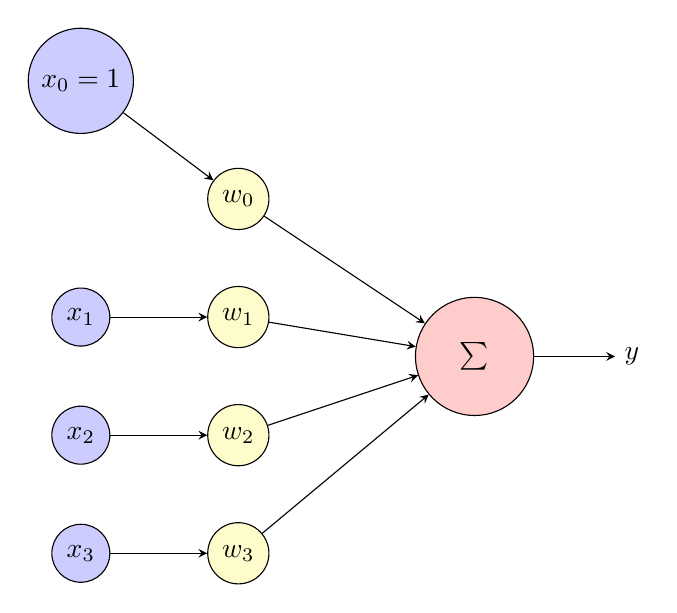
\begin{tikzpicture}[>=stealth]
    % Input nodes
    \node[draw, circle, fill=blue!20] (input0) at (0,4) {$x_0=1$}; % bias as input node
    \foreach \i in {1,2,3}
        \node[draw, circle, fill=blue!20] (input\i) at (0,2.5-\i*1.5) {$x_\i$};
        
    % Weight nodes
    \foreach \i in {0,...,3}
        \node[draw, circle, fill=yellow!20] (weight\i) at (2,2.5-\i*1.5) {$w_\i$};
        
    % Output node
    \node[draw, circle, fill=red!20, minimum size=1.5cm] (output) at (5,0.5) {$\sum$};
    
    % Output label node
    \node (outputLabel) at (7,0.5) {$y$};

    % Connections from input nodes to weight nodes
    \foreach \i in {0,...,3}
        \draw[->] (input\i) -- (weight\i);
    
    % Connections from weight nodes to output node
    \foreach \i in {0,...,3}
        \draw[->] (weight\i) -- (output);
    
    % Connection from output node to output label
    \draw[->] (output) -- (outputLabel) node[midway, above] {};
\end{tikzpicture}
\end{center}

    \caption{Visual diagram of a perceptron with bias term as $w_0$}
    \label{fig:perceptron}
\end{figure}

\subsection{Algorithm Overview} \label{def:PLA}
The Perceptron Learning Algorithm (PLA) is a binary classifier that attempts to find a separating hyperplane for data points. This hyperplane is determined by the weight vector \( \mathbf{w} \) and a bias \( b \). The algorithm iteratively adjusts the weights to classify the data points correctly.

\begin{figure}[H]
    \centering
    \includegraphics[width=0.5\textwidth]{img/pla-plot.png}
    \caption{Linearly Separable Data}
    \label{fig:pla-plot}
\end{figure}

\begin{definitionbox}{PLA Algorithm Steps}
    \begin{enumerate}
    \item \textbf{Initialisation}: Begin with a random weight vector \( \mathbf{w} \).
    \item \textbf{While there exists a misclassified data point}: 
    \begin{itemize}
        \item For \( y \in \{-1, +1\} \): If \( \text{sign}(\mathbf{w}^\top \textbf{x} _i) \neq y_i \) then update the weights:
        \[
        \mathbf{w} \leftarrow \mathbf{w} + y_i x_i
        \]

    \end{itemize}
    \item Repeat until all data points are correctly classified or a set number of iterations is reached.
\end{enumerate}

\end{definitionbox}



\subsection{Intuition}
\subsubsection{Visualising the Decision Boundary}
Imagine a 2D plane with two types of points: red and blue. The perceptron seeks a line where all red points lie on one side and all blue points on the other. The equation for such a line is:
\[ ax + by + c = 0 \]

\noindent
This can be represented more generally for higher dimensions as:
\[ \mathbf{w}^\top\mathbf{x} = 0 \]
where $\mathbf{w}$ is the weight vector and $\mathbf{x}$ is the input feature vector.


\noindent
Note that we do not specify a bias term, which for our 2D example, is the y-intercept.

\subsubsection{Learning with the Perceptron Algorithm}
Begin with an arbitrary weight vector $\mathbf{w}$. For each data point $\mathbf{x}_i$, the prediction $h(\mathbf{x}_i, \mathbf{w})$ is determined by the sign of $\mathbf{w}^T\mathbf{x}_i$. If this prediction aligns with the actual label $y_i$, no adjustments are made. Otherwise, the weights are updated to better classify the data point:
\[ \mathbf{w} \leftarrow \mathbf{w} + y_i\mathbf{x}_i \]

\subsubsection{Interpreting the Weight Vector}
The weight vector $\mathbf{w}$ sets the orientation of the separating hyperplane (or line, in 2D). It can be thought of as a vector perpendicular to this plane (or line, in 2D). The quantity $\mathbf{w}^T\mathbf{x}$ computes the position of point $\mathbf{x}$ relative to the origin, along the direction of $\mathbf{w}$. The sign indicates which side of the plane $\mathbf{x}$ lies on.\\

\noindent
When updating $\mathbf{w}$, the separating hyperplane shifts to better classify the misclassified data point $\mathbf{x}_i$.

\subsubsection{Equation for Weight Update}
To comprehend the weight update rule, consider the following equation:

\begin{align*}
y_i\cdot\mathbf{w}^{\prime\top}\mathbf{x}_i &= y_i\cdot(\mathbf{w}+y_i\mathbf{x}_i)^\top\mathbf{x}_i \\
&= y_i\cdot\mathbf{w}^\top\mathbf{x}_i + y_i^2\cdot\mathbf{x}_i^\top\mathbf{x}_i \\
&= y_i\cdot\mathbf{w}^\top\mathbf{x}_i + \|\mathbf{x}_i\|^2
\end{align*}

\begin{itemize}
    \item \( \mathbf{w'} \) is the updated weight vector after the weight adjustment rule has been applied. It is defined as \( \mathbf{w'} = \mathbf{w} + y_i\mathbf{x}_i \).
    \item The dot product \( \mathbf{w}^\top\mathbf{x}_i \) measures the alignment between the weight vector and the input feature vector. It gauges how close or far the point \( \mathbf{x}_i \) is from being correctly classified.
    \item The term \( y_i \) signifies the true class of the data point.
     \item \( y_i \cdot \mathbf{w}^\top\mathbf{x}_i \) is positive when the data point \( \mathbf{x}_i \) is correctly classified as the signs of  $\mathbf{w}^\top \mathbf{x}_i$ and $y_i$ match.
    \item \( y_i \cdot \mathbf{w}^\top\mathbf{x}_i \) is negative when the data point \( \mathbf{x}_i \) is misclassified  as the signs of  $\mathbf{w}^\top \mathbf{x}_i$ and $y_i$ do not match.
    \item If the point \( \mathbf{x}_i \) is misclassified, the weights need adjustment in the direction of \( y_i \mathbf{x}_i \). This term \( y_i\mathbf{x}_i \) acts as the corrective factor to guide the update. Remember, our goal is to have a positive  \( y_i \cdot \mathbf{w}^\top\mathbf{x}_i \) that is large (see next section on maximising the margin.)
    \item As \( y_i^2 \) is always positive (because \( y_i \) is either +1 or -1), the term \( \|\mathbf{x}_i\|^2 \) always has a positive contribution during the update, indicating that the magnitude of the feature vector plays a consistent role in the update.
    \item The updated weight vector \( \mathbf{w'} \) becomes more aligned with the misclassified point, improving future predictions.
    \item An animated diagram can be found \href{https://upload.wikimedia.org/wikipedia/commons/a/aa/Perceptron_training_without_bias.gif}{here}:

\end{itemize}


\subsection{Maximising the Margin}
The aim of the Perceptron is to maximise the margin by which points are classified. When adjusting the weight vector \( \mathbf{w} \) using a misclassified point \( x_i \), the updated weight vector \( \mathbf{w'} \) is more aligned with \( x_i \) in the direction of the correct label \( y_i \). This ensures that the product \( y_i \cdot \mathbf{w'}^T x_i \) becomes larger, leading to a more robust decision boundary with larger margins.

\subsection{Considering Bias}
So far we have considered instances of a 2D perceptron where every revision of the algorithm redraws a hyperplane line that passes through the origin. \\

\noindent
To consider the set of all possible hyperplanes in $\mathbb{R}^2$ is possible to redefine the hyperplane to be $\textbf{w}^\top \mathbf{x} + b = 0 $, so the hyperplane no longer has to pass through the origin, leaving us with a new algorithm.


\begin{enumerate}
    \item \textbf{Initialisation}: Begin with a random weight vector \( \mathbf{w} \) and bias \( b \).
    \item \textbf{While there exists a misclassified data point}: 
    \begin{itemize}
        \item For \( y \in \{-1, +1\} \): If \( \text{sign}(\mathbf{w}^\top \textbf{x} _i + b) \neq y_i \) then update the weights:
        \[
        \mathbf{w} \leftarrow \mathbf{w} + y_i x_i
        \]

        \item And update the bias:
        \[ b' = b + y_i \]

    \end{itemize}
    \item Repeat until all data points are correctly classified or a set number of iterations is reached.
\end{enumerate}

\noindent
To simplify computation, we can implement bias as part of $\textbf{w}$ by increasing the dimensions of $\textbf{w}$ by one, and setting $x_0$ to 1 and $w_0$ to the bias. Then we use the algorithm in \ref{def:PLA}




\subsection{Remarks}
The Perceptron Learning Algorithm will stop after a finite number of iterations if the data is linearly separable. Otherwise, it requires an external stopping condition, such as a predefined maximum number of iterations, or it chooses the hyperplane with minimal misclassification errors (Pocket Algorithm)

\section{Linear Regression}
Linear regression is a supervised learning algorithm primarily used for modelling the relationship between a scalar dependent variable and one or more independent variables. In the context of classification, linear regression can be applied to predict continuous values which are then thresholded to produce discrete class labels.

\subsection{Regression Error}
Given a dataset with $n$ samples, the regression error $\hat{R}_n(h)$ is defined as the average squared difference between the predicted and actual values:

\begin{align}
    \hat{R}_n(h) &= \frac{1}{n} \sum_{i=0}^{n} (h(\textbf{w}, \textbf{x}_i) - y_i)^2 \\
    \hat{R}_n(\textbf{w}) &= \frac{1}{n} \sum_{i=0}^{n} (\textbf{w}^\top \textbf{x}_i - y_i)^2 \\ \label{eq:regerror}
    &= \frac{1}{n} ||X\textbf{w} - \textbf{y}||^2
\end{align}

where:
\begin{itemize}
    \item $X$ is the data matrix where each row $x_i^T$ represents a sample.
    \item $y$ is the label vector.
\end{itemize}

\subsection{Closed-Form Solution (Least-Squares)}
The optimal weight vector $w$ that minimises the regression error can be found by setting the gradient of $\hat{R}_n(w)$ to zero:

\begin{align*}
    \nabla \hat{R}_n(w) &= 0 \\
    \begin{aligned}
        &\text{From \eqref{eq:regerror} we differentiate} \\
        &\frac{2}{n}X^\top(X\textbf{w} - \textbf{y}) = 0 \\
        &X^\top X\textbf{w} = X^\top \textbf{y}
    \end{aligned}
\end{align*}

\begin{definitionbox}{Closed-Form Solution for Least-Squares}
From the above, the solution for $\textbf{w}$ is:

$$
    \textbf{w} = (X^\top X)^{-1} X^\top \textbf{y}
$$
    
\end{definitionbox}


Here, $(X^\top X)^{-1} X^\top$ is known as the Moore-Penrose pseudoinverse of $X$. 

\subsection{Classifier Thresholding}
Once $\textbf{w}$ is found, predictions can be made for new data points. In the context of classification, the predicted continuous values can be thresholded (e.g., at 0.5 for binary classification) to produce discrete class labels.









\chapter{Learning and Generalisation}
\section{Probably Approximately Correct (PAC) Learning: Terms}
\begin{enumerate}
    \item A is impossible: $P(A) = 0$
    \item A is certain: $P(A) = 1$
    \item A is almost certain: $P(A) \approx 1$
    \item A is probable: $(P(A) > 0) \wedge (P(A) < 1)$
    \item A is correct if error $\varepsilon_A = 0$
    \item A is approximately correct: $\varepsilon_A \approx 0$, very small
    \item A is probably (how certain?) correct: $P(\varepsilon_A = 0) \approx 1$
    \item A is probably approximately correct (P.A.C.): $P(\varepsilon_A > B)$ with $B \approx 1$
\end{enumerate}

\section{Hoeffding's Inequality}

Hoeffding's Inequality is a foundational result in probability theory and statistics, especially within machine learning and statistical learning theory. It offers bounds on the probability that the sample mean of independent and identically distributed (i.i.d.) random variables deviates from its expected value.

\begin{sidenotebox}{Statement of Hoeffding's Inequality (General Case)}

For a sequence of independent and bounded random variables $X_1, X_2, \ldots, X_n$, each lying in the range $a \leq X_i \leq b$, the sample mean $\bar{X}$ adheres to the following inequality:

\begin{equation}
P\left(\left|\bar{X} - \mu\right| \geq \epsilon\right) \leq 2\exp\left(-\frac{2n\epsilon^2}{(b - a)^2}\right)
\end{equation}

Where:
\begin{itemize}   
\item  $\bar{X}$ represents the sample mean.
\item  $\mu$ denotes the true expected value of $X_i$.
\item  $a$ and $b$ are the respective lower and upper bounds of $X_i$.
\item  $\epsilon$ indicates the deviation from the expected value.
\item  $n$ is the sample count.
\end{itemize}
\end{sidenotebox}


\begin{sidenotebox}{Derivation of Hoeffding's Inequality for Binary Classification}
Note to self: proof from https://nowak.ece.wisc.edu/SLT07/lecture7.pdf is much cleaner and concise. Replace

\subsubsection{Preliminaries}
Given independent random variables \(X_1, X_2, \ldots, X_n\) where each \(i\) satisfies \(a_i \leq X_i \leq b_i\), define \(S_n = \sum_{i=1}^{n} X_i\) and \(E[S_n] = \sum_{i=1}^{n} E[X_i]\).

\subsubsection{Theorem: Chernoff Bound}
For any positive \(t\):
\begin{align*}
\mathbb{P}(S_n - E[S_n] \geq \epsilon) &\leq \mathbb{P}(e^{tS_n} \geq e^{t(E[S_n] + \epsilon)}) \\
&\leq \frac{\mathbb{E}[e^{tS_n}]}{e^{t(E[S_n] + \epsilon)}}
\end{align*}
Given the independence of the \(X_i\)'s:
\begin{align*}
\mathbb{E}[e^{tS_n}] &= \mathbb{E}\left[\exp\left(t\sum_{i=1}^{n} X_i\right)\right] \\
&= \prod_{i=1}^{n} \mathbb{E}[e^{tX_i}]
\end{align*}

\subsubsection{Exponential Moments}
Considering that for \(0 \leq \lambda \leq 1\), \(e^x \leq \lambda e^{\frac{x}{\lambda}} + (1-\lambda)\):
\begin{align*}
\mathbb{E}[e^{tX_i}] &\leq \mathbb{E}\left[\lambda e^{\frac{ta_iX_i}{\lambda}} + (1-\lambda)e^{\frac{tb_iX_i}{1-\lambda}}\right] \\
&= \lambda e^{\frac{ta_i}{\lambda}} + (1-\lambda)e^{\frac{tb_i}{1-\lambda}}
\end{align*}

\subsubsection{Combine and Optimise}
Starting from our earlier result using the Chernoff bound:
\[ \mathbb{P}(S_n - E[S_n] \geq \epsilon) \leq \frac{\mathbb{E}[e^{tS_n}]}{e^{t(E[S_n] + \epsilon)}} \]

And using the exponential moments bound we derived:
\[ \mathbb{E}[e^{tX_i}] \leq \lambda e^{\frac{ta_i}{\lambda}} + (1-\lambda)e^{\frac{tb_i}{1-\lambda}} \]

Substituting in, we get:
\[ \mathbb{E}[e^{tS_n}] \leq \prod_{i=1}^{n} \left( \lambda e^{\frac{ta_i}{\lambda}} + (1-\lambda)e^{\frac{tb_i}{1-\lambda}} \right) \]

The optimization step involves selecting values of \(t\) and \(\lambda\) that minimize the right-hand side of this inequality, given our constraints. For Hoeffding's inequality, in the context of binary classification, where \(a_i = 0\) and \(b_i = 1\), we optimize for this specific case – this step is non-trivial.\\


Substituting the exponential moments into the Chernoff bound and performing optimization over \(t\) and \(\lambda\), we get:
\begin{align*}
\mathbb{P}(S_n - E[S_n] \geq \epsilon) &\leq \exp\left(-\frac{2\epsilon^2}{\sum_{i=1}^{n} (b_i - a_i)^2}\right)\\
\mathbb{P}(\bar{X} - \mu \geq \epsilon) &\leq 2\exp\left(-\frac{2\epsilon^2n}{(b - a)^2}\right)
\end{align*}
To account for both sides of the deviation (positive and negative), we multiply the right-hand side by 2, arriving at the given form of Hoeffding's inequality.
\end{sidenotebox}


\subsection{Hoeffding's Inequality}
Using Hoeffding's inequality, we can then write:

\begin{definitionbox}{Hoeffding's Inequality}
\[
P\left(\left|\widehat{R}_n(h) - R(h)\right| \geq \epsilon\right) \leq 2\exp\left(-2n\epsilon^2\right)
\]

\begin{itemize}
    \item \(\widehat{R}_n(h)\) - The empirical risk or empirical error rate of hypothesis \(h\), which is the average error over a sample of size \(n\). This is our training data.
    \item \(R(h)\) - The true risk or true error rate of hypothesis \(h\), which represents the expected error rate over all possible instances.
    \item \(n\) - The sample size or the number of instances tested against the hypothesis \(h\).
\end{itemize}


\end{definitionbox}

Which provides a bound on the probability that the empirical risk deviates from the true risk by at least \(\epsilon\).

\subsection{Understanding Hoeffding's Inequality through the Dice-Roll example}

Hoeffding's Inequality provides a bound on the probability that the sum of independent, bounded random variables deviates from its expected value. To get an intuitive understanding, let's consider the simple example of rolling a fair six-sided dice.\\


Given a fair six-sided dice, each face has an equal probability of $\frac{1}{6}$ of landing. Thus, the expected value, \( E[X] \), of a single dice roll is:

\[ E[X] = \frac{1}{6}(1) + \frac{1}{6}(2) + \frac{1}{6}(3) + \frac{1}{6}(4) + \frac{1}{6}(5) + \frac{1}{6}(6) = 3.5 \]


Now, let's roll the dice \( n \) times and compute the average, \( \bar{X}_n \), of the rolls. As we roll the dice more and more, we expect \( \bar{X}_n \) to get closer to the expected value, 3.5.

Hoeffding's Inequality states that for any \( \epsilon > 0 \):

\[ P(|\bar{X}_n - E[X]| > \epsilon) \leq 2 \exp\left(-2n\epsilon^2\right) \]

This means the probability that our average deviates from the expected value by more than \( \epsilon \) decreases exponentially as the number of rolls, \( n \), increases. In simpler terms, the more we roll the dice, the closer our average gets to 3.5, and the probability of a significant deviation becomes very small.\\

For instance, if after rolling the dice 1000 times our average is 3.4 or 3.6 (which is \( \epsilon = 0.1 \) away from 3.5), Hoeffding's Inequality gives an upper bound on how likely this event is. And as mentioned, the more rolls we have, the tighter this bound becomes, ensuring our empirical average approaches the true expected value.\\

Hoeffding's Inequality gives us a formal, mathematical guarantee on the convergence of empirical averages to their expected values, as demonstrated with our dice roll example.






\section{Probability vs. Expectation}
For any event, there exists a true probability, denoted by \( P(\text{event}) \), and an expectation, denoted by \( \mathbb{E}[\text{event}] \). While one might anticipate these to be approximately equal, in many cases (e.g., polls), they can significantly differ. \\

We notate the as $p_{\text{event}} = P(\text{event})$ and $e_{\text{event}}$ = $\mathbb{E}[\text{event}]$ \\

One example:\\

Imagine that there is a small town with only 100 voters and two candidates running for mayor: Alice and Bob. A polling company does a survey and finds the following probabilities for voter preference:

\begin{itemize}
    \item 50\% of voters prefer Alice.
    \item 45\% of voters prefer Bob.
    \item 5\% of voters are undecided.
\end{itemize}

If we only consider the probabilities, one might simply conclude that Alice is more likely to win since she has a higher percentage of voter preference.\\

Now, expectation: suppose in reality, the undecided voters are learning towards Bob because of a recent positive news story about him, and 80\% of the undecided voters will go for Bob and 20\% for Alice.\\

For Alice:
\begin{align*}
    \text{Expected votes} &= (\text{Probability of Alice}) \times (\text{Total voters}) \\
    &\quad + (\text{Probability of undecided}) \times (\text{Probability of choosing Alice}) \times (\text{Total voters}) \\
    &= 0.50 \times 100 + 0.05 \times 0.20 \times 100 \\
    &= 50 + 1 \\
    &= 51 \text{ votes}
\end{align*}

For Bob:
\begin{align*}
    \text{Expected votes} &= (\text{Probability of Bob}) \times (\text{Total voters}) \\
    &\quad + (\text{Probability of undecided}) \times (\text{Probability of choosing Bob}) \times (\text{Total voters}) \\
    &= 0.45 \times 100 + 0.05 \times 0.80 \times 100 \\
    &= 45 + 4 \\
    &= 49 \text{ votes}
\end{align*}

Even considering the expected swing from the undecided voters towards Bob, Alice still has a higher expected vote count. However, the gap has narrowed considerably when we take the expected behaviour of undecided voters into account. The initial probabilities alone would not have shown us this nuance.

\begin{commentbox}{Author's Comment on Probability vs Expectation}
In machine learning (or at least, this module), the expectation is used to refer to the ground truth (in our example, this is the actual expected outcomes of the election), which we are trying to approximate with our samples of training data (which is the poll in our example). Our model was not complex enough to account for undecided voters swinging to either Alice or Bob, despite our approximation turning out correct in the end.
\end{commentbox}

\subsection{Hoeffding's Inequality in Learning}
Hoeffding's inequality offers a bound on how the empirical average (or empirical risk) of i.i.d. random variables deviates from its expectation. For any \( \epsilon > 0 \):
\begin{align*}
P(e_{\text{event}} - p_{\text{event}} > \epsilon) & \leq \delta \\
P(e_{\text{event}} - p_{\text{event}} \leq \epsilon) & \leq e^{-2\epsilon^2n} \quad \text{(one-sided)} \\
P(|e_{\text{event}} - p_{\text{event}}| > \epsilon) & \leq 2e^{-2\epsilon^2n} \quad \text{(two-sided)}
\end{align*}

An important implication of Hoeffding's inequality is the concept of being \textit{Probably Approximately Correct (PAC)}. In the realm of machine learning, this means that our empirical estimates are likely close to the true values, but not always exact.\\

\begin{definitionbox}{Empirical and True risk}
In the context of learning, we denote:
\begin{itemize}
    \item \( \widehat{R}_n(h) \): Empirical risk (training error), which is the approximation of the true risk based on our training data set. This is our $p_{\text{event}}$.
    \item \( R(h) \): True risk (test error), which is the expectation of the error over the entire probability distribution of the data. This is the ground truth, which in practice, we do not have access to. This is our $e_{\text{event}}$.
\end{itemize}
    
\end{definitionbox}
With Hoeffding's inequality, we can assert that:
$$
P(|\widehat{R}_n(h) - R(h)| > \epsilon) \leq 2e^{-2\epsilon^2n}
$$
This showcases the closeness of the training error to the test error, given sufficient samples.


\subsection{Assumptions}
One critical assumption for Hoeffding's inequality to hold is that the data samples \( x \) are independent and identically distributed (i.i.d.). This means that each data sample is drawn independently from the same distribution \( P(\mathcal{X}) \). This assumption ensures that the empirical averages are meaningful estimates of the true averages.

\section{Error Measures in Learning}

The core of learning theory revolves around approximating an unknown target function using available data. The degree of approximation is quantified using error measures, also referred to as loss functions.

\subsection{Error Measures or Loss Functions}
Given a hypothesis class \( \mathcal{H} \) and a target function, it is crucial to quantify how well a chosen hypothesis \( h \) approximates the target. Loss functions measure the discrepancy between the predictions made by \( h \) and the actual values:
\begin{itemize}
    \item \textbf{Squared Error}: \( \ell(y, \widehat{y}) = (y - \widehat{y})^2 \)
    \item \textbf{Binary Error}: \( \ell(y, \widehat{y}) = \mathbb{I}(y \neq \widehat{y}) \)
\end{itemize}

\subsection{Training vs. Test Error}
The training error measures the discrepancy on the dataset used to find \( h \), while the test error gives an expectation of the error on new, unseen data:
\begin{align*}
    \text{Training Error:} \quad & R_{\text{in}}(h) = \frac{1}{n} \sum_{i=1}^{n} \ell(h(x_i), y_i) \\
    \text{Test Error:} \quad & R(h) = \mathbb{E}[\ell(h(x), y)]
\end{align*}

$\ell$ is the error function that depends on what type of machine learning methods we are using.

\subsection{Error Costs and Decision Making}
In some scenarios, different types of errors might incur different costs. For instance, in medical diagnosis, a false negative (diagnosing a diseased patient as healthy, for example) might have a more severe consequence than a false positive (diagnosing a healthy patient as diseased). 

\subsection{Error Costs in Machine Learning}
The process of learning in machine learning models involves minimising errors based on certain criteria. Depending on the specific problem and requirements, different error costs can be considered.

\begin{itemize}
    \item \textbf{Equally Penalising Errors:} In some scenarios, all types of errors, be it false positive or false negative, are penalised equally.
    \item \textbf{Aggressively Penalising False Negatives:} In critical scenarios such as medical diagnosis, a false negative (failing to detect a disease when it is present) could have dire consequences, and hence is penalised heavily.
    \item \textbf{Risk Aversion by Penalising False Positives:} In other situations, such as spam email detection, false positives (classifying legitimate email as spam) might be more costly.
\end{itemize}

\subsection{Binary Error and the Indicator Function}\label{indicatorfunc}
The binary error, which checks if the predicted output matches the actual output, uses the indicator function. The function is defined as:
\[
\mathbb{I}(a \neq b) = 
\begin{cases} 
1 & \text{if } a \neq b \\
0 & \text{otherwise}
\end{cases}
\]
In the context of learning, the binary error is used to check if the hypothesis $h(x)$ is equal to the true function value $f(x)$. If they are not equal, the error is 1, otherwise it is 0.

\begin{table}[H]
\centering
\begin{tabular}{|c|c|c|}
\hline
& $f = +1$ & $f = -1$ \\
\hline
$h = +1$ & No error & False positive \\
\hline
$h = -1$ & False negative & No error \\
\hline
\end{tabular}
\caption{Two types of error}
\end{table}

The two primary types of errors are:
\begin{itemize}
    \item \textbf{False Negative (Type I error)}: The model rejects a scenario when it should have accepted it.
    \item \textbf{False Positive (Type II error)}: The model accepts a scenario when it should have rejected it.
\end{itemize}

\subsection{Penalizing Errors}

\begin{table}[H]
\centering
\begin{tabular}{|c|c|c|}
\hline
& $f = +1$ & $f = -1$ \\
\hline
$h = +1$ & 0 & 1 \\
\hline
$h = -1$ & 1 & 0 \\
\hline
\end{tabular}
\caption{Equally penalizing errors}
\end{table}

\begin{table}[H]
\centering
\begin{tabular}{|c|c|c|}
\hline
& $f = +1$ & $f = -1$ \\
\hline
$h = +1$ & 0 & 100 \\
\hline
$h = -1$ & 1 & 0 \\
\hline
\end{tabular}
\caption{Risk averse: false positive is expensive}
\end{table}

\begin{table}[H]
\centering
\begin{tabular}{|c|c|c|}
\hline
& $f = +1$ & $f = -1$ \\
\hline
$h = +1$ & 0 & 1 \\
\hline
$h = -1$ & 100 & 0 \\
\hline
\end{tabular}
\caption{Aggressive: false negative is expensive}
\end{table}



Different penalties can be assigned to each type of error based on the requirements of the specific application. For example, in scenarios like medical diagnosis, a false negative might be heavily penalised.

\begin{commentbox}{Author's Comment on Semantics of `Risk Averse' and `Aggressive'}
    Note that this module uses `risk averse' to discourage false positives and `aggressive' to discourage false negatives, in practice this terminology can vary. It is more precise to describe models based on their preference for minimising one type of error over the other, or for being balanced in treating both types of errors.
\end{commentbox}



\section{Probabilistic Learning Framework}
\subsection{Considering Noise, Learning with Noisy Data (Stochastic Noise)}\label{learning_with_noise}
\begin{commentbox}{Note to Reader: Module Arrangement}
    The module notes defines the grounds for probabilistic learning here, but does not elaborate further until the next chapter where we apply these concepts.
\end{commentbox}


Machine learning, in practice, often faces the challenge of having to deal with inherent uncertainties present in real-world data, in the form of noise. \\

Instead of a deterministic output \( y = f(x) \), the relationship may be probabilistic \( y \sim P(y|x) \), allowing for the same input to yield different outputs.\\

Data points \( (x, y) \) are generated from a joint distribution \( P(x, y) \), which can be decomposed as:

$$ P(x,y) = P(y|x)P(x) $$


We model noise in the data as 

$$ y = f(x) + N $$

where $N$ is noise, $f(x) = \mathbb{E}[y|x]$  and $\mathbb{E}[N|x] = 0$. \\

An example would be $y=w^\top x + N$ where $N \sim \mathcal{N}(0, \Sigma)$ is independent of $x$. \\

In the special case of the deterministic problem, there is zero noise $N= 0$ and $P(y|x)$ is concentrated on the single form f(x).

\subsection{Errors and the Learning Setup}

To make the most accurate predictions, the choice of an optimal hypothesis function \( h \) is influenced by both the nature of noise in the data and the form of the loss function used to measure prediction errors.

\begin{itemize}
    \item \textbf{Squared Error Loss:} When using squared error loss, denoted by \( \ell(y, \widehat{y}) = (y - \widehat{y})^2 \), the optimal decision rule \( g(x) \) is the one that minimises the expected squared error, $\mathbb{E}[(y-h(x))^2|x]$ across the data distribution. Formally, it is the expected value of the target variable given the input, \( g(x) = \mathbb{E}[y|x] \).
    
    \item \textbf{Binary Error Loss:} For classification tasks where the error is binary, expressed as \( \ell(y, \widehat{y}) = \mathbb{I}(y \neq \widehat{y}) \) where \( \mathbb{I} \) is the indicator function, the optimal hypothesis \( g(x) \) is that which maximizes the probability of the correct label being chosen. In mathematical terms, \( g(x) \) is the class that has the maximum posterior probability given the input, \( g(x) = \underset{y}{\arg\max}\, P(y|x) \).
\end{itemize}

This subsection emphasises the reliance of the optimal decision on the choice of the loss function, whether it is for regression with squared error or for classification with binary error, taking into account the statistical properties of the data.


We aim to develop a model to make accurate predictions or decisions based on input data amidst noise. This process involves selecting an appropriate hypothesis from a set of potential candidates. 

\begin{definitionbox}{Learning Setup Overview}
    

\begin{itemize}
    \item \textbf{Input and Output:} The learning algorithm receives an input \( x \in \mathcal{X} \) and predicts an output \( y \in \mathcal{Y} \). The true relationship between inputs and outputs is governed by the unknown probability distribution \( P(y|x) \), which the learning algorithm tries to approximate.
    $$ \{(x_1, y_1), (x_2, y_2), \ldots, (x_n, y_n)\}  \sim P$$
    
    \item \textbf{Data:} We collect a dataset \( \{(x_1, y_1), (x_2, y_2), \ldots, (x_n, y_n)\} \) which is assumed to be sampled from the joint distribution \( P(x, y) \). This dataset serves as the empirical basis for learning the input-output mapping.
    
    \item \textbf{Hypothesis Class:} The hypothesis class \( \mathcal{H} \) is the set of all functions \( h: \mathcal{X} \rightarrow \mathcal{Y} \) that the learning algorithm considers. The choice of \( \mathcal{H} \) can significantly impact the algorithm's ability to generalise from the training data to unseen data.
    $$
    \mathcal{H} \subset \{h:\mathcal{X} \rightarrow \mathcal{Y}\}
    $$
    
    \item \textbf{Loss Function:} The loss function \( \ell: \mathcal{Y} \times \mathcal{Y} \rightarrow \mathbb{R} \) quantifies how far off a prediction is from the actual value. It provides a criterion for evaluating the quality of a hypothesis.
    
    \item \textbf{Learning Objective:} The goal of learning is to find a hypothesis \( g \in \mathcal{H} \) that best approximates the true distribution \( P(y|x) \). Formally, we seek a hypothesis that minimises the expected loss over the data distribution: 
    $$ g = \arg\min_{h \in \mathcal{H}} \mathbb{E}[\ell(h(x), y)] $$
    
    \item \textbf{Aggregation Strategy:} While the expectation is a common way to aggregate the loss over the distribution, alternative strategies may be required in certain situations, such as when the distribution \( P \) is highly imbalanced. This consideration is crucial for ensuring that the model performs well across all segments of the data, not just the majority class.
\end{itemize}

\end{definitionbox}

The process of choosing \( \mathcal{H} \) is non-trivial and depends on several factors, including the complexity of the data, the type of problem (regression or classification), and the computational resources available. This choice determines the hypothesis space within which our optimal model will be found and, consequently, the success of our learning algorithm in making accurate predictions.\\

For a fixed single hypothesis $h \in \mathcal{H}$, the learning process uses the familiar Hoeffding's Inequality:

\begin{itemize}
    \item \textbf{Training Error (Empirical Risk):} The training error is the average loss over the training set, and it is denoted by \( \widehat{R}_n(h) \). For a training set of size \( n \), it is defined as:
    \[
    \widehat{R}_n(h) = \frac{1}{n} \sum_{i=1}^{n} \ell(h(x_i), y_i);
    \]
    where \( \ell \) is the loss function, \( h(x_i) \) is the prediction of hypothesis \( h \) for input \( x_i \), and \( y_i \) is the true output.

    \item \textbf{Test Error (Out-of-Sample Risk):} The test error is the expectation of the loss function over the joint distribution of inputs and outputs. It is denoted by \( R(h) \) and represents the true risk of hypothesis \( h \). It can be expressed in two ways:
    \begin{itemize}
        \item \( R(h) = \mathbb{P}(h(x_i) \neq f(x_i)); \)
        \item \( R(h) = \mathbb{E}[\widehat{R}_n(h)]; \)
    \end{itemize}
    where \( f \) is the true function that we are trying to approximate. The test error is a measure of how well the hypothesis generalises to new data that were not seen during training.
\end{itemize}

Again as usual, by Hoeffding's Inequality:
\[
P\left(\left|\widehat{R}_n(h) - R(h)\right| \geq \epsilon\right) \leq 2\exp\left(-2n\epsilon^2\right)
\]

The discrepancy between training error and test error relates the concept of overfitting, where a hypothesis may perform well on the training data but poorly on new data due to its failure to generalise.




\subsection{Generalisation for Multiple Hypotheses}
When working with a hypothesis class \( \mathcal{H} \), we are often interested in the performance of not just one, but all hypotheses within this class, so we can choose the best model from the class set. To extend Hoeffding's inequality to the entire class, we employ the union bound. This approach provides a way to aggregate the probabilities of multiple independent events, extending the Hoeffding's inequality to handle multiple hypotheses.\\

     Let \( \mathcal{H} = \{h_1, h_2, \ldots, h_M\} \) be a finite hypothesis class with \( M \) distinct hypotheses. The probability that at least one hypothesis \( h \in \mathcal{H} \) has a large deviation between its empirical risk \( \widehat{R}_n(h) \) and true risk \( R(h) \) is given by the union bound:

    \[P\left( \bigcup_{m=1}^{M} \{ |\widehat{R}_n(h_m) - R(h_m)| > \varepsilon \} \right) = 
    P\left( \max_{h \in \mathcal{H}} |\widehat{R}_n(h) - R(h)| > \varepsilon \right) \leq \sum_{m=1}^{M} P\left( |\widehat{R}_n(h_m) - R(h_m)| > \varepsilon \right).
    \]

    Using Hoeffding's inequality for each hypothesis, we have:

    \[
    P\left( |\widehat{R}_n(h_m) - R(h_m)| > \varepsilon \right) \leq 2e^{-2n\varepsilon^2},
    \]

    which gives us the union bound for all \( M \) hypotheses:

    \begin{equation}
    P\left( \max_{h \in \mathcal{H}} |\widehat{R}_n(h) - R(h)| > \varepsilon \right) \leq 2Me^{-2n\varepsilon^2}.
    \label{eq:union_bound}
    \end{equation}

    \begin{commentbox}{Why take the union bound?}
        The union bound is taken as a worst-case scenario approach to probability. When dealing with multiple hypotheses, we want to ensure that our bound on the generalisation error holds not just for a single hypothesis but for all hypotheses in our class.\\

        In the context of machine learning, each hypothesis could potentially overfit the training data and not generalise well to new, unseen data. The union bound helps us assess this risk across all hypotheses by combining their individual risks. This way, we can make a statement like "with high probability, none of the hypotheses will have a generalisation error greater than some specified bound," giving us confidence that the hypothesis we select from this class will perform well on new data.
    \end{commentbox}

     To understand the square root and logarithm in the derived bound, we define \( \delta \) such that \( \delta = 2Me^{-2n\varepsilon^2} \), leading to \( \varepsilon = \sqrt{\frac{1}{2n}\log\frac{2M}{\delta}} \). This rearrangement comes from solving the equation for \( \varepsilon \) in terms of \( \delta \) and \( M \) (the number of hypotheses). \\


\begin{definitionbox}{Multiple Hypotheses Generalisation Bound}    
     Thus, with probability at least \( 1 - \delta \), for all hypotheses \( h \in \mathcal{H} \) simultaneously, we have:
    \[
    |\widehat{R}_n(h) - R(h)| \leq \sqrt{\frac{1}{2n}\log\frac{2M}{\delta}}
    \]
\begin{itemize}
    \item \( \widehat{R}_n(h) \) is the empirical risk of the hypothesis \( h \), calculated from the training data.
    \item \( R(h) \) is the true risk of the hypothesis \( h \), considering the entire data distribution.
    \item \( M \) represents the size of the hypothesis class \( \mathcal{H} \)
    \item \( \delta \) is a parameter that controls the confidence level of the bound: with probability at least \( 1 - \delta \), the bound holds.
    \item \( n \) is the size of the training data.
\end{itemize}

This inequality is a statement about the uniform convergence of the empirical risk to the true risk for all hypotheses in the class.\\

More specifically, it shows, that with high probability, the true risk of any hypothesis in the class will not deviate from the empirical risk observed on the training data by more than the bound on the RHS.\\

The RHS probabilistic bound $ \sqrt{\frac{1}{2n}\log\frac{2M}{\delta}}$ is the difference between empirical risk and true risk for any hypothesis within the hypothesis class.\\

This also means that if we minimise empirical risk, we are likely to be close to minimising true risk, which is our goal.


\end{definitionbox}



\subsection{Empirical Risk Minimisation (ERM)}

Empirical Risk Minimisation (ERM) is a principle used to select a hypothesis from a hypothesis class \( \mathcal{H} \) based on empirical (test) data. Let us denote the optimal hypothesis in \( \mathcal{H} \) by \( h^* \), which is the hypothesis that minimises the true risk \( R(h) \):

\begin{equation*}
    h^* = \arg\min_{h\in\mathcal{H}} R(h).
\end{equation*}

The aim of ERM is to choose a hypothesis \( g \) from \( \mathcal{H} \) that has the smallest empirical error:

\begin{equation*}
    g = \arg\min_{h\in\mathcal{H}} \widehat{R}_n(h),
\end{equation*}

where \( \widehat{R}_n(h) \) is the empirical risk calculated from the training data.\\

Note that we don't know what is hypothesis $h^*$ because we cannot practically measure true risk $R(h^*)$ (we don't have infinite data samples). But we can calculate empirical risk $\widehat{R}_n{h}$ and therefore identify hypothesis $g$. \\




With the empirical risk minimiser \( g \), we wish to understand how well it approximates the optimal hypothesis \( h^* \) in terms of the true risk. The following bound provides this guarantee:


\begin{definitionbox}{Risk of the Empirical Risk Minimiser}
With probability at least \( 1 - \delta \),

\begin{equation*}
    R(g) - R(h^*) \leq \sqrt{\frac{2 \log \frac{2M}{\delta}}{n}},
\end{equation*}

where \( M \) is the size of the hypothesis class \( \mathcal{H} \), and \( n \) is the size of the sample.\\

Note that the absolute value is no longer needed because $R(g) - R(h^*)$ is always positive, since we assume $h^*$ is the best hypothesis and has the lowest error. Also, note that we are taking the difference in true risk.

\begin{itemize}
    \item Hypothesis \( h^* \) is the optimal hypothesis that has the smallest true risk \( R_n(h^*) \) for the entire data distribution.
    \item Hypothesis \( g \) is the hypothesis we can identify and choose, that has the smallest empirical risk \( \widehat{R}_n(g) \) for our training data.
\end{itemize}

\end{definitionbox}


\textbf{The principle of ERM suggests a practical way to approximate the best possible prediction rule (hypothesis) within the hypothesis class $\mathcal{H}$, based on observed data. \\}

To understand this relationship, the size of this class, denoted by \( M \), directly affects how well the model generalises. A larger \( \mathcal{H} \) implies a more complex model space, which, while potentially leading to a lower empirical risk, can also increase the risk of overfitting. \\

From equation \ref{eq:union_bound}:

\begin{align}
P\left( \max_{h \in \mathcal{H}} |\widehat{R}_n(h) - R(h)| > \varepsilon \right) \leq 2Me^{-2n\varepsilon^2} \label{eq:extension_hoeff_M} \\
P\left(|\widehat{R}_n(g)-R(g)|>\varepsilon\right)\leq 2|\mathcal{H}|e^{-2\varepsilon^2n}
\end{align}


We want a hypothesis that fits the training data well (minimising empirical risk) but also generalise to new, unseen data (minimising true risk).
The complexity of $\mathcal{H}$, quantified by its cardinality \( |\mathcal{H}| \), affects the likelihood of the empirical risk mirroring the true risk.\\


For any fixed hypothesis \( h \in \mathcal{H} \), the probability that the empirical risk deviates from the true risk by more than an amount \( \varepsilon \) is bounded by \( 2e^{-2n\varepsilon^2} \), which reassures us about the stability of the hypothesis:

\[
P\left(|\widehat{R}_n(h)-R(h)|>\varepsilon\right)\leqslant2e^{-2\varepsilon^2n}
\]

However, when we consider a hypothesis \( g \) that has been chosen based on the data (such as one that minimises the empirical risk), we need to account for the selection process from within the hypothesis class. Here, the bound adjusts to include the size of the class, reflecting the added uncertainty from this selection:

\[
P\left(|\widehat{R}_n(g)-R(g)|>\varepsilon\right)\leqslant2|\mathcal{H}|e^{-2\varepsilon^2n}
\]

So we can conclude that $g$ cannot deviate too far from $h^*$, using the data we have.

% \subsection{Choosing the hypothesis}

% The bounds and guarantees discussed provide a foundation for understanding the role of the hypothesis class in the learning process.accurate and robust against overfitting. These theoretical insights are crucial for practical machine learning, where the ultimate goal is to achieve reliable predictions on real-world, unseen data.


% \subsection{Choosing our Hypothesis: Linear Classification Example}


% \subsubsection*{Feature Representation}
% In linear classification, we typically represent features as vectors:
% \begin{equation*}
%     \mathbf{x} = (x_1, \ldots, x_d) \in \mathbb{R}^d
% \end{equation*}
% where \( x_0 = 1 \) is often included to account for the bias term, thus extending the vector into \( \mathbb{R}^{d+1} \).

% \subsubsection*{Labels and Data Points}
% The labels are denoted by \( y \) and can take on values in the set \( \{+1, -1\} \), corresponding to the two classes. We consider \( n \) data points:
% \begin{equation*}
%     (\mathbf{x}_1, y_1), \ldots, (\mathbf{x}_n, y_n),
% \end{equation*}
% where each \( \mathbf{x}_i \) is a feature vector and \( y_i \) is its associated label.

% \subsubsection*{Hypothesis Class}
% The hypothesis class consists of functions parameterised by weight vectors \( \mathbf{w} \):
% \begin{equation*}
%     h_{\mathbf{w}}(\mathbf{x}) = \text{sign}(\mathbf{w}^{\top}\mathbf{x}),
% \end{equation*}
% where \( \mathbf{w} = (w_0, w_1, \ldots, w_d) \) and the sign function returns +1 or -1 depending on the sign of its argument.

% \subsubsection*{The Perceptron Algorithm}
% The perceptron algorithm seeks a hypothesis \( h \in \mathcal{H} \) such that \( h(\mathbf{x}_i) = y_i \) for all \( i = 1, \ldots, n \), assuming such a hypothesis exists within the hypothesis class. The empirical risk minimizer under this setting is:
% $$
%     g = \arg\min_{h \in \mathcal{H}} \sum_{i=1}^{n} \mathbb{I}(h(\mathbf{x}_i) \neq y_i),
% $$
% which corresponds to minimising the number of misclassifications. See \ref{indicatorfunc} for more information on the indicator function $\mathbb{I}$.

\subsubsection*{Applicability of ERM Theory}
When considering ERM in the context of linear classification, a critical question arises: Is the hypothesis class \( \mathcal{H} \) finite? \\

In theory, there are infinite amount of possible weights, as they can take on any real-valued numbers. This is clearly not computable with our current setup – The finiteness of \( \mathcal{H} \) is important for the guarantees of ERM to hold, otherwise the bounds will not be useful (infinitely large $|\mathcal{H}|$ on the RHS of the bound does not give us confidence that the LHS error will be bounded.). In later sections we learn to find a more practical quantity for the number of hypotheses.\\



\section{Growth Function, Shattering, and Break Points}
\subsection{Overlapping Hypotheses Example}\label{overlap_hypo}

\begin{figure}[ht]
    \centering
    \includegraphics[width=0.4\textwidth]{img/h-overlap.png}
    \caption{Hypotheses that split the points similarly}
    \label{fig:h-overlap}
\end{figure}

In practical machine learning applications, especially in classification problems, we sometimes encounter the situation where two different hypotheses \( h_1 \) and \( h_2 \) provide similar predictions over the training set. This is referred to as overlapping hypotheses. Mathematically, if \( h_1 \approx h_2 \) then it follows that:

\begin{equation*}
    \widehat{R}_n(h_1) \approx \widehat{R}_n(h_2) \quad \text{and} \quad R(h_1) \approx R(h_2),
\end{equation*}

where \( \widehat{R}_n(h) \) represents the empirical risk and \( R(h) \) represents the true risk of a hypothesis \( h \). This indicates that when the hypotheses are similar, their empirical and true risks are expected to be close to each other. Thus:

\begin{equation*}
    |\widehat{R}_n(h_1) - R(h_1)| \approx |\widehat{R}_n(h_2) - R(h_2)|,
\end{equation*}

which implies that a large difference in empirical risk between \( h_1 \) and \( h_2 \) can often indicate a similarly large difference in their true risks. This is an important concept for understanding the performance of learning algorithms. However, it is important to realise that \( h_1 \neq h_2 \) if there exists some \( \textbf{x} \in \mathcal{X} \) where $\mathcal{X}$ is the input space, such that \( h_1(\textbf{x}) \neq h_2(\textbf{x}) \); this is what creates a dichotomy, or a configuration of dividing points, in the hypothesis space.

\[
\left|\widehat{R}_n(h_1) - R(h_1)\right| > \varepsilon \text{ often implies } \left|\widehat{R}_n(h_2) - R(h_2)\right| > \varepsilon
\]

\[
h_1 \neq h_2 \text{ if } \exists \textbf{x} \in \mathcal{X} : h_1(\textbf{x}) \neq h_2(\textbf{x}) \rightarrow \text{ dichotomy}
\]

This is why we only considered a finite sample of $\textbf{x}$ from the input space $\mathcal{X}$ – more than one hypothesis could represent the same dichotomy for a finite amount of points.  


\subsection{Growth Function and Perceptron}

In this section we consider the perspective of including a finite sample of data, $\textbf{x}$ from the input space $\mathcal{X}$.\\

We propose the growth function, a function which quantifies the capacity of a hypothesis class \( \mathcal{H} \) to fit data. It is a function of the number of points \( n \) and is denoted as \( m_{\mathcal{H}}(n) \). This function counts the maximum number of dichotomies—or distinct classifications—of \( n \) points that the hypothesis class can realise. For the perceptron, which is a linear classifier, this function is closely related to the concept of `shattering`.

\begin{definitionbox}{Growth Function}\label{growth_func}
The growth function measures the number maximum number of dichotomies that a hypothesis class can produce on any set of $n$ points from the input space. Intuitively, it tells us how many ways the hypothesis class can label $n$ points, regardless of their actual arrangement in the input space.\\

The growth function for a hypothesis class \( \mathcal{H} \), denoted by \( m_{\mathcal{H}}(n) \), represents the maximum number of dichotomies that can be realised by the hypotheses in \( \mathcal{H} \) on any set of \( n \) points. For a perceptron, this is bounded by the number of hypotheses, and can be formalised as:

\begin{equation*}
    m_{\mathcal{H}}(n) = \max_{\textbf{x}_1,\ldots,\textbf{x}_n \in \mathcal{X}} |\mathcal{H}(\textbf{x}_1, \ldots, \textbf{x}_n)| \leq 2^n,
\end{equation*}

where \( \mathcal{H}(\textbf{x}_1, \ldots, \textbf{x}_n) \) denotes the set of all possible dichotomies on \( n \) points. However, not all sets of points can be shattered by a perceptron, especially if the data is not linearly separable. \\

Note that the upper bound for the growth function is $2^n$ – the maximum number of ways $n$ points can be classed positively or negatively. 
\end{definitionbox}

\begin{definitionbox}{Dichotomies in Machine Learning}
    A dichotomy refers to a particular way of splitting or labelling a set of points into two categories, typically represented as positive (+1) and negative (-1) classes. Dichotomies are used to describe the different possible classifications that a set of data points can have according to the hypotheses within the class.
\end{definitionbox}


\subsection{Shattering and break points}



\begin{definitionbox}{What does it mean to `shatter' (in the context of the perceptron)?}
A set of points is considered to be `shattered` by the hypothesis class \( \mathcal{H} \) if, for every possible binary labelling of these points, there exists a hypothesis in \( \mathcal{H} \) that can produce exactly these labels. The `break point` is the smallest number of points that the hypothesis class cannot shatter, signifying a limit to the complexity of \( \mathcal{H} \).
\end{definitionbox}

\begin{definitionbox}{The Break Point}
    The break point is the smallest number \( k \) such that no set of \( k \) points can be shattered by the hypothesis class \( \mathcal{H} \). For a perceptron, the break point provides insight into the complexity and capacity of the model.\\

    \textbf{Break Point} (capacity of \(\mathcal{H}\)): There exists \( k \) such that \( m_{\mathcal{H}}(k) < 2^k \) which is the size of the largest set \( \{x_1, \ldots, x_k\} \) in \(\mathcal{X}\) that can be shattered by \(\mathcal{H}\).

    \[\exists k:m_{\mathcal{H}(k)}\nexists(\mathbf{x_1},\ldots,\mathbf{x_k})\in\mathcal{X}:\text{shattered by }\mathcal{H})\]

\end{definitionbox}

% \begin{figure}[H]
%     \centering
%     \includegraphics[width=1\textwidth]{img/shatter-dich.png}
%     \caption{2D perceptron shattering configurations}
%     \label{fig:shatter-dich}
% \end{figure}
\begin{figure}[h!]
    \centering
    \begin{subfigure}[b]{0.2\textwidth}
        \centering
        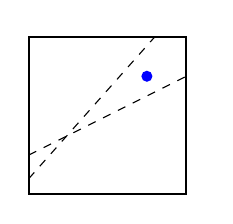
\begin{tikzpicture}
            \draw[thick] (-1,-1) rectangle (1,1);
            \fill[blue] (0.5,0.5) circle (2pt);
            \draw[dashed] (-1,-0.5)--(1,0.5) node[right] {};
            \draw[dashed] (-1,-0.8)--(0.6,1) node[right] {};
        \end{tikzpicture}
        \caption{Shattering 1 point}
    \end{subfigure}
    \hfill
    \begin{subfigure}[b]{0.2\textwidth}
        \centering
        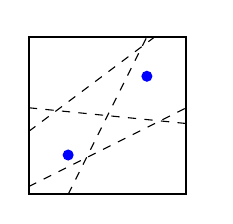
\begin{tikzpicture}
            \draw[thick] (-1,-1) rectangle (1,1);
            \fill[blue] (-0.5,-0.5) circle (2pt);
            \fill[blue] (0.5,0.5) circle (2pt);
            \draw[dashed] (-1,0.1)--(1,-0.1) node[right] {};
            \draw[dashed] (-1,-0.9)--(1,0.1) node[right] {};
            \draw[dashed] (-1,-0.2)--(0.6,1) node[right] {};
            \draw[dashed] (-0.5,-1)--(0.5,1) node[right] {};
        \end{tikzpicture}
        \caption{Shattering 2 points}
    \end{subfigure}
    \hfill
    \begin{subfigure}[b]{0.2\textwidth}
        \centering
        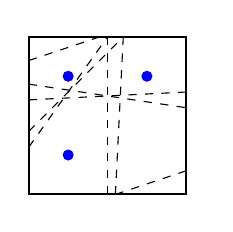
\begin{tikzpicture}
            \draw[thick] (-1,-1) rectangle (1,1);
            \fill[blue] (0.5,0.5) circle (2pt);
            \fill[blue] (-0.5,0.5) circle (2pt);
            \fill[blue] (-0.5,-0.5) circle (2pt);
            \draw[dashed] (-1,-0.4)--(0,1) node[right] {};
            \draw[dashed] (-1,-0.2)--(0.2,1) node[right] {};
            \draw[dashed] (-1,0.2)--(1,0.3) node[right] {};
            \draw[dashed] (-1,0.4)--(1,0.1) node[right] {};
            \draw[dashed] (0,1)--(0,-1) node[right] {};
            \draw[dashed] (0.2,1)--(0.1, -1) node[right] {};
            \draw[dashed] (1,-0.7)--(0.1, -1) node[right] {};
            \draw[dashed] (-1,0.7)--(-0.1,1) node[right] {};
        \end{tikzpicture}
        \caption{Shattering 3 points}
    \end{subfigure}
    \hfill
    \begin{subfigure}[b]{0.2\textwidth}
        \centering
        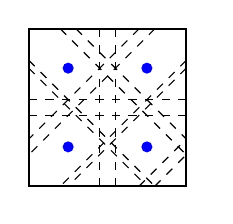
\begin{tikzpicture}
            \draw[thick] (-1,-1) rectangle (1,1);
            \fill[blue] (0.5,0.5) circle (2pt);
            \fill[blue] (0.5,-0.5) circle (2pt);
            \fill[blue] (-0.5,0.5) circle (2pt);
            \fill[blue] (-0.5,-0.5) circle (2pt);
            \draw[dashed] (-1,0.1)--(1,0.1) node[right] {};
            \draw[dashed] (-1,-0.1)--(1,-0.1) node[right] {};
            \draw[dashed] (0.1,1)--(0.1,-1) node[right] {};
            \draw[dashed] (-0.1,1)--(-0.1,-1) node[right] {};
            \draw[dashed] (0.4,1)--(-1,-0.4) node[right] {};
            \draw[dashed] (0.6,1)--(-1,-0.6) node[right] {};
            \draw[dashed] (1,0.6)--(-0.6,-1) node[right] {};
            \draw[dashed] (1,0.5)--(-0.5,-1) node[right] {};

            \draw[dashed] (-0.4,1)--(1,-0.4) node[right] {};
            \draw[dashed] (-0.6,1)--(1,-0.6) node[right] {};
            \draw[dashed] (-1,0.6)--(0.6,-1) node[right] {};
            \draw[dashed] (-1,0.5)--(0.5,-1) node[right] {};

            
            
            


            \draw[dashed] (0.4,-1)--(1,-0.4) node[right] {};
            \draw[dashed] (0.6,-1)--(1,-0.6) node[right] {};
            

        \end{tikzpicture}
        \caption{Shattering 4 points}
    \end{subfigure}
    \caption{Perceptron shattering points on a 2D plane.}
    \label{fig:2d_perceptron}
\end{figure}

\begin{itemize}
    \item Given a 2D perceptron and a single point, the single point can be classified as +1 or -1. The total number of dichotomies, $m_\mathcal{H}(1)$, is 2. The 2D perceptron can shatter a single point.
    \item Given a 2D perceptron and two points, either both points are +1 or -1, or they are one of each. There are 4 dichotomies, $m_\mathcal{H}(2)= 4$. The 2D perceptron can shatter two points.
    \item A 2D perceptron can fully shatter a maximum of 3 points, unless they are collinear, in which case some separations are not possible. Still, the maximum number of dichotomies are 8, $m_\mathcal{H}(2)= 8$
    \item Once you have four points, they can be geometrically considered as the vertices of a convex quadilateral. Labelling opposite vertices with the same class show that no single line can separate the classes. So four points cannot be shattered, so 4 is the break point for a 2D perceptron. Still, there are 14 possible dichotomies, $m_\mathcal{H}(4)=14  $
\end{itemize}

A 2D perceptron can fully shatter a maximum of 3 points, unless they are collinear, in which case some separations are not possible.\\

We then introduce the notion of the Combinatorial Quantity function:
\subsection{The Combinatorial Quantity \( B(N, k) \)}\label{combinatorial_quantity}

\begin{commentbox}{Note to Self: Notation check}
    Is $B(N,k)$ referring to the combinatorial quantity for a perceptron, or is it general? Please fix notation soon
\end{commentbox}

This is a measure of how many dichotomies can you list on \( N \) points so that no \( k \) are shattered. $k$ is the break point, defined in the previous section. Intuitively, it is the list of all possible combinations, `$N$ choose $i$', or $\textbf{C}_i^N$, for values of $i$ up to $k-1$.

\[ B(N, k): \text{Max. number of dichotomies on } N \text{ points so that no } k \text{ are shattered.} \]

\begin{table}[h!]
\centering
\begin{tabular}{|c|c|c|}
\hline
\( X_1 \) & \( X_2 \) & \( X_3 \) \\
\hline
\Circle   & \Circle   & \Circle   \\
\Circle   & \Circle   & \CIRCLE   \\
\Circle   & \CIRCLE   & \Circle   \\
\CIRCLE   & \Circle   & \Circle   \\
\CIRCLE   & \CIRCLE   & \Circle   \\
\Circle   & \CIRCLE   & \CIRCLE      \\
\CIRCLE   & \Circle   & \CIRCLE      \\
\hline
\end{tabular}
\quad
\begin{tabular}{|c|c|c|c|}
\hline
\( X_1 \) & \( X_2 \) & \( X_3 \) &\( X_4 \) \\
\hline
\Circle & \Circle & \Circle & \Circle \\
\Circle & \Circle & \Circle & \CIRCLE \\
\Circle & \Circle & \CIRCLE & \Circle \\
\Circle & \CIRCLE & \Circle & \Circle \\
\CIRCLE & \Circle & \Circle & \Circle \\
\hline
\end{tabular}
\caption{Visualisation of dichotomies for \( B(3,3) \) and \( B(4,2) \). \(B(3,3) = 5, B(4,2) = 5 \)}
\end{table}

It is easy to see that \[ B(N, k) \leq \sum_{i=0}^{k-1} \binom{N}{i} . \]
Note we use the inequality for the combinatorial quantity function – an easy example why we do this is because not every hypothesis class can achieve every combination. For example, in Figure \ref{fig:2d_perceptron}, for the 2D perceptron with four points and break point 4, there are only 14 possible dichotomies. If we enumerated the general case using our visualisation in \ref{combinatorial_quantity}, we could get up to $\textbf{C}^4_3+\textbf{C}^4_2+\textbf{C}^4_1+\textbf{C}^4_0 = 15$, which is greater than 14.

\begin{sidenotebox}{Bound of Combinatorial Quantity Function}\label{combquant_function_bound}
\textbf{Theorem (actually a form of the Sauer-Shelah Lemma)}
\[ B(N, k) \leq \sum_{i=0}^{k-1} \binom{N}{i} . \]

\textbf{Proof Sketch}
(Induction on \(N\).)
\begin{enumerate}
    \item Verify for \(N = 1\): \( B(1,1) \leq 1 \) \checkmark
    \item Suppose \( B(N, k) \leq \sum_{i=0}^{k-1} \binom{N}{i} \).
\end{enumerate}

\textbf{Lemma (Pascal's Identity)}
\[ \binom{N}{k} + \binom{N}{k-1} = \binom{N+1}{k} . \]

    



Then,
\begin{align*}
B(N + 1, k) &\leq B(N, k) + B(N, k - 1) \\
&\leq \sum_{i=0}^{k-1} \binom{N}{i} + \sum_{i=0}^{k-2} \binom{N}{i} \\
&= 1 + \sum_{i=1}^{k-1} \left( \binom{N}{i} + \binom{N}{i-1} \right) \quad (\text{by lemma}) \\
&= 1 + \sum_{i=1}^{k-1} \binom{N+1}{i} \\
&= \sum_{i=0}^{k-1} \binom{N+1}{i}
\end{align*}

A clearer explanation of the recurrence relation can be watched \href{https://youtu.be/6FWRijsmLtE?si=Tg2jX1YDYAjXFdE0&t=372}{here}, courtesy of the Caltech ML Lectures. \\

\textbf{To show the bound is polynomial in k:}
\[ B(N, k) \leq \sum_{i=0}^{k-1} \binom{N}{i} . \]
\begin{align*}
    \sum_{i=0}^{k-1} \binom{N}{i} \leq \left(\frac{N}{k-1}\right)^{k-1} \sum_{i=0}^{k-1} \binom{k-1}{i} \left(\frac{k-1}{N}\right)^i\\
\leq \left(\frac{N}{k-1}\right)^{k-1} \sum_{i=0}^{k-1} \binom{k-1}{i} \left(\frac{k-1}{N}\right)^m\\
\leq \left(\frac{N}{k-1}\right)^{k-1} \left(1 + \frac{k-1}{N}\right)^m\\
\leq \left(\frac{N}{k-1}\right)^{k-1} e^{k-1} \\
\end{align*}


\end{sidenotebox}

We show the combinatorial quantity \( B(N, k) \) is polynomial. So for the perceptron and any other ML methods that have a finite break point, the growth function $m_\mathcal{H}$  is polynomial as well.  \\

Also, we realise that $B(N,k)$ is actually the general growth function that tells you the total number of possible dichotomies for a given number of data points $N$ and break point k. The growth function $m_\mathcal{H}(n)$ tells you the total number of possible dichotomies for a hypothesis $\mathcal{H}$ that has a pre-determined constant $k$ that we don't have to show, for $n$ points.\\

From Hoeffding's Inequality in \ref{eq:extension_hoeff_M}:

\begin{align*}
P\left( \max_{h \in \mathcal{H}} |\widehat{R}_n(h) - R(h)| > \varepsilon \right) \leq 2Me^{-2n\varepsilon^2} 
=_{\text{somewhat, but not quite}}P\left( \sup_{h \in \mathcal{H}} |\widehat{R}_n(h) - R(h)| > \varepsilon \right) \leq 2m_{\mathcal{H}}(n)e^{-2n\varepsilon^2}
\end{align*}

Here, we've tried replacing the count of hypotheses $M$ with the growth function, $m_{\mathcal{H}}(n)$, which bounds the numbers of ways $\mathcal{H}$ can label any set of $n$ points.
This step is motivated by the realisation that not all hypotheses in $\mathcal{H}$ are distinct when considering how they label a finite set of points – many hypotheses might make the same predictions, so the true ``size" of $\mathcal{H}$ with respect to the dataset is better captured by $m_{\mathcal{H}}(n)$ than $M$. \\

Note that what we did was merely to illustrate our understanding, but we actually cannot simply interchange $M$ with the growth function. Through a lot more technicality and change of constants, we can produce the Vapnik-Chervonenkis inequality which is sound. This is covered further in the Caltech lectures \href{https://youtu.be/6FWRijsmLtE?si=fP-5cgJ52UhqAIGI&t=3484}{here}.\\


Earlier in \ref{growth_func}, we could define the growth function $m_{\mathcal{H}}$ having an upper bound of $2^n$.\\

This is unfortunately not low enough, because having an exponential $n$ within the bound will interfere with the $e^{-2n\epsilon^2}$ part for large $n$, and we cannot be sure that the difference between empirical and true error will be bounded.\\

However, since we can show that $m_{\mathcal{H}}$ is polynomial, we have no problems with the right-hand-side bound because the $e^{-2n\epsilon^2}$ part overrules the $m_{\mathcal{H}}(n)$.

\begin{itemize}
    \item If there is no break point, the growth function \( m_{\mathcal{H}}(n) \) is equal to \( 2^n \), which is the maximum number of dichotomies possible for binary classification on \( n \) points.
    \item If a break point \( k \) exists, \( m_{\mathcal{H}}(k) \) is polynomial in \( n \), indicating that the number of dichotomies is less than the maximum, thus reflecting a constraint in the hypothesis class. This is because $\mathcal{O}(2^n) > \mathcal{O}(n^k)$.
    \item Such a polynomial is expressed as \( m_{\mathcal{H}}(k) = a_kn^k + a_{k-1}n^{k-1} + \ldots + a_1n + a_0 \), where the coefficients \( a_i \) correspond to the complexity of dichotomies at different levels.

\end{itemize}

The notes stop short of a detailed proof for going from Hoeffding's inequality to the Vapnik-Chernovenkis inequality, yet they present us with an equation that, while not entirely precise, serves as an illustrative stepping stone toward understanding the Vapnik-Chernovenkis Inequality.




\subsection{The Vapnik-Chervonenkis Inequality}\label{vc-ineq-subsection}



We can consider the VC-dimension, which is a measure of the capacity or complexity of a classification algorithm. More specifically, the VC-dimension, denoted as \( d_{VC}(\mathcal{H}) \), measures the capacity of \( \mathcal{H} \) by the size of the largest set of points that can be shattered by \( \mathcal{H} \). The VC inequality refines the generalisation bound by incorporating the VC-dimension of the hypothesis class into the extended Hoeffding's inequality.
\begin{definitionbox}{Vapnik-Chervonenkis Inequality}
    \begin{equation*}
P\left(\sup_{h\in\mathcal{H}}|\widehat{R}_{n}(h)-R(h)|>\varepsilon\right)\leqslant4\underbrace{m_{\mathcal{H}}(2n)}_{\leqslant(2n+1)^{d_{VC}(\mathcal{H})}}e^{-\varepsilon^{2}n/8}
\end{equation*}

Where $d_{VC}(\mathcal{H})=\max\{n : m_{\mathcal{H}}(n) = 2^n\}$ is the VC-dimension
\end{definitionbox}


A finite VC dimension implies that as the number of data points \( n \) grows, the empirical risk \( \widehat{R}_n(g) \) converges to the true risk \( R(g) \) for the chosen hypothesis \( g \), ensuring that the learning process is effective and that the model will likely generalise well to unseen data with a high probability \( 1 - \delta \).

\begin{itemize}
    \item The growth function is related to the VC-dimension by the Sauer-Shelah Lemma, which bounds $m_{\mathcal{H}}(n)$ by a polynomial of degree $d_{VC}(\mathcal{H})$ when $n \geq d_{VC}(\mathcal{H})$.
    \item The VC inequality implies that a finite VC-dimension is sufficient for a hypothesis class to generalize well, given enough data points.
\end{itemize}

\begin{commentbox}{What's the VC Dimension?}
The module does not really go into this, but it is helpful to draw the difference between the VC Dimension and the growth function $m_\mathcal{H}(n)$. Here is a summary of what we have covered so far:

\begin{itemize}
    \item The growth function $m_{\mathcal{H}}(n) $ measures the maximum number of dichotomies that a hypothesis class $\mathcal{H}$ can implement on any set of $n$ points, for a given hypothesis class.
    \item The general growth function $B(N,k)$ measures the maximum number of dichotomies for $N$ points, and a given break point $k$. This works for any kind of hypothesis class that you know the break point $k$ for.
    \item The VC Dimension measures the maximum number of points that can be shattered by the hypothesis class. It only indicates whether the general growth function, $B(N, k)$, is equal to or smaller than $2^k$.
    
\end{itemize}
The VC dimension of a hypothesis class $\mathcal{H}$, denoted as $VC(\mathcal{H})$, is defined by

 \[d_{VC}(\mathcal{H})=\max\{n : m_{\mathcal{H}}(n) = 2^n\}\]

 This is quite easy to see with our 2D perceptron example in \ref{combinatorial_quantity}. It is the greatest $n$ where we can shatter all points– simply one minus the break point – as we know, for a 2D perceptron, we can shatter a max of 3 points with a break point at 4. So the VC dimension would be 3.\\

It is the tipping point where the hypothesis class's capacity to perfectly classify every possible scenario is exceeded by the complexity of the task.

 In our example, at some point, our perceptron gets bad at clustering many datapoints, but this shows that our hypothesis set (and thus our growth function) is limited in size, and we can learn because the maximum difference between true risk and empirical risk is bounded by the VC-inequality.



\begin{sidenotebox}{Relating the Two}
By the Sauer–Shelah lemma (see \ref{combquant_function_bound}):
If $d_{VC}(\mathcal{H}) = k-1$, then for all $k$:
\begin{align*}
B(H, k) &\leq \sum_{i=0}^{d} \binom{m}{i}\\
&\leq \left(\frac{N}{k-1}\right)^{k-1} e^{k-1}
\end{align*}


From our example in in \ref{combinatorial_quantity}, this is the generalised rule. The right hand side form is familiar within Figure \ref{fig:vc_dimension_plot}.
\end{sidenotebox}
\begin{sidenotebox}{Theoretically infinite VC dimensions}
    Let's have fun with an extreme example – we want to use logistic regression to fit a set of points. We want to have a function that draws a line between points, and if the line passes through a point, it is classed as $+1$ and if not, $-1$. (We will cover logistic regression properly in another chapter).\\

    We could naively consider the set of all polynomial functions over the real numbers. Since polynomials can wiggle an arbitrary number of times, given $d$ points on a plane, you can always find a polynomial of degree at least $d-1$ that will pass through any $d$ points with classification combination, totalling $2^d$. So $m_{\mathcal{H}}(n) = 2^n$ for all n, and by definitition of $d_{VC}$ maximising $n$ takes us to infinity. (This is coincidentally an infinitely large hypothesis set).\\

    But what we have shown is just illegally excessive, over-astronomical overfitting on a maximum, and it goes to show that the exponential case is when you choose too large a hypothesis set that guarantees overfitting every point.
\end{sidenotebox}

    
\end{commentbox}


\begin{figure}[H]
    \centering
    \includegraphics[width=0.5\textwidth]{img/vc-plot.png}
    \caption{The relationship between the probability of deviation and the number of samples, illustrating how the VC-dimension affects the generalisation bound. A higher VC-dimension or fewer samples increase the probability bound, indicating a lower confidence in generalisation.}
    \label{fig:vc_dimension_plot}
\end{figure}

The graph above shows how the bound on the generalisation error decreases with the number of samples $N$, for different values of the VC-dimension. It emphasises the trade-off between the complexity of the hypothesis class (as measured by the VC-dimension) and the amount of data required to ensure good generalisation with high probability.\\

\textbf{Rule of Thumb:}
A common heuristic is that the number of training examples $n$ should be at least an order of magnitude greater than the VC-dimension, i.e., $n \geq 10d_{VC}(\mathcal{H})$, to provide reasonable confidence in the generalisation of the learned hypothesis.


\subsection{Generalisation Error in the Context of the VC Inequality}

The VC Inequality provides a bound on the generalisation error for machine learning models. It establishes that with a high probability, the true risk \(R(h)\) for any hypothesis \(h\) from the hypothesis class \(\mathcal{H}\) will not be much higher than the empirical risk \(\widehat{R}_n(h)\), up to a complexity term that depends on the VC dimension of the hypothesis class.

\begin{definitionbox}{VC Inequality Error}\label{vc_inequality_error}
\[P\left(\sup_{h\in\mathcal{H}}|\widehat{R}_{n}(h)-R(h)|>\varepsilon\right)\leqslant4\underbrace{m_{\mathcal{H}}(2n)}_{\leqslant(2n+1)^{d_{VC}(\mathcal{H})}}e^{-\varepsilon^{2}n/8}\]
From the VC Inequality, we get a term for error on the rightmost square root term:

\[
R(h) \leq \widehat{R}_n(h) + \sqrt{\frac{8d_{VC}(\mathcal{H})}{n} \log\left(\frac{2n + 1}{\delta}\right) + \frac{8}{n} \log\frac{4}{\delta}}
\]

This error is called a complexity term, denoted as a function of $\Omega$ where:
\[
\Omega(n, \mathcal{H}, \delta ) = \sqrt{\frac{8d_{VC}(\mathcal{H})}{n} \log\left(\frac{2n + 1}{\delta}\right) + \frac{8}{n} \log\frac{4}{\delta}}
\]
\end{definitionbox}

This bound indicates that as the number of samples \(n\) increases, the gap between empirical risk and true risk closes, provided the VC dimension \(d_{VC}\) remains fixed.

\subsection{Performance vs. Complexity}

The graph below illustrates the trade-off between a model's complexity and its performance. The complexity is represented by the VC dimension, and the error is depicted on the vertical axis. 

\begin{figure}[H]
\centering
\includegraphics[width=0.8\textwidth]{img/perf-vs-cmplxty.png} % path to your image file
\caption{The trade-off between model complexity and performance. The blue curve represents the training error which decreases with model complexity, while the red curve represents the test error which initially decreases and then increases due to overfitting. The point where the test error is minimum corresponds to the optimal model complexity.}
\label{fig:performance_vs_complexity}
\end{figure}

As the VC dimension increases, the training error typically decreases as the model becomes more capable of fitting the training data. However, beyond a certain point, an increase in complexity leads to overfitting, and the test error begins to increase. The optimal VC dimension, \(d_{VC}^*\), is the point at which the test error is minimised, striking a balance between underfitting and overfitting.


\subsection{Polynomial Bounds on the Growth Function}

The growth function, denoted as \(m_{\mathcal{H}}(n)\), describes the maximum number of distinct outputs (or dichotomies) that a hypothesis class \(\mathcal{H}\) can produce for any sample of size \(n\). Understanding the behaviour of this function is key for assessing the capacity of the hypothesis class to fit various datasets.

Polynomial bounds on the growth function provide a way to approximate the complexity term \(\Omega(n, \mathcal{H}, \delta)\) in generalisation error bounds. Specifically:

\begin{itemize}
  \item The growth function \(m_{\mathcal{H}}(k)\) is bounded by a polynomial in \(n\), with the VC dimension acting as a break point. This means that for any sample size \(n\), the growth function \(m_{\mathcal{H}}(n)\) is at most polynomial in \(n\), which is significant as it limits the number of dichotomies the hypothesis class can shatter.
  
  \item When \(n\) is less than the VC dimension \(d_{VC}\), \(m_{\mathcal{H}}(n)\) can grow as fast as \(2^n\). However, once \(n\) exceeds \(d_{VC}\), the growth of \(m_{\mathcal{H}}(n)\) is significantly constrained, reflecting the limitations imposed by the finite VC dimension.
  
  \item A common polynomial bound is given by \(m_{\mathcal{H}}(n) \leq n^{d_{VC}} + 1\), which simplifies the expression and is more convenient to use than the exact polynomial form involving coefficients.
  
  \item For sufficiently large \(n\), an even tighter bound is often used:
  \[
  m_{\mathcal{H}}(n) \leq \left(\frac{ne}{d_{VC}}\right)^{d_{VC}}
  \] 
  where \(e\) is the base of the natural logarithm. This bound is known to be a more accurate estimate for the growth function when the sample size is large relative to the VC dimension (note that it is in a very similar form to the derivation in \ref{combquant_function_bound}).
\end{itemize}

These polynomial bounds are instrumental in deriving generalisation bounds such as those presented by the VC inequality, which connects the empirical risk with the true risk of a hypothesis.

\begin{examplebox}{Example Learning Question}
    In a binary classification problem, the test error is 27\% on 100 random test samples. Give a confidence interval that contains the expected test error with 90\% probability? How does the result change if the test error is obtained on 1000 samples? Use Hoeffding, and then VC assuming VC dimension of the hypothesis class is 3.\\

Let $X_i \in \{0,1\}$ denote the error in classifying sample $i$, $n$ the number of samples (100 or 1000), $\mu = \mathbb{E}[X_i]$ the expected test error, and $\nu = \frac{1}{n}\sum_{i=1}^{n} X_i = 0.27$ the empirical test error.\\

By Hoeffding's inequality,
\[ P(|\nu - \mu| \geq \epsilon) \leq 2e^{-2n\epsilon^2}. \]\\

Therefore, $\mu \in [\nu - \epsilon, \nu + \epsilon]$ with probability at least $1 - \delta = 1 - 2e^{-2n\epsilon^2}$. Setting $1 - \delta = 0.9$ and solving for $\epsilon$ we get $\epsilon = \sqrt{\log(2/\delta)/(2n)}$, which gives $\epsilon \approx 0.12$ for $n = 100$ and $\epsilon \approx 0.04$ for $n = 1000$. The required confidence intervals are approximately $[0.15, 0.39]$ for $n = 100$ and $[0.23, 0.31]$ for $n = 1000$.\\

Repeat with Vapnik-Chervonenkis Inequality:
\[ P(|\nu - \mu| \geq \epsilon) \leq 4(2n + 1)^{d_{VC}}e^{-\frac{n\epsilon^2}{8}}. \]\\

Given $\nu = 0.27$ and $d_{VC} = 3$, we want to solve for $\epsilon$.\\

We start by rearranging the inequality to solve for $\epsilon^2$:
\[ \epsilon^2 = \frac{8}{n} \log\left(\frac{4(2n + 1)^{d_{VC}}}{\delta}\right). \]\\

Substituting $d_{VC} = 3$ and for $n = 100$ and $1000$ samples, we can compute the specific values of $\epsilon$. 

\end{examplebox}

\begin{examplebox}{Inequality Bounds Question}
Given VC inequality \( P\left( \sup_{h\in\mathcal{H}} |\widehat{R}_n(h) - R(h)| > \epsilon \right) \leq 4m_{\mathcal{H}}(2n)e^{-\frac{n\epsilon^2}{8}} \), show how to arrive at the following generalisation bounds \( R(h) \leq \widehat{R}_n(h) + \Omega(n, \mathcal{H}, \delta) \):

\begin{itemize}
    \item[(a)] \(\Omega(n, \mathcal{H}, \delta) = \sqrt{\frac{8d_{VC}}{n} \log(2n + 1) + \frac{8}{n} \log \frac{4}{\delta}}\)
    \item[(b)] \(\Omega(n, \mathcal{H}, \delta) = \sqrt{\frac{8d_{VC}}{n} \log \frac{2ne}{d_{VC}} + \frac{8}{n} \log \frac{4}{\delta}}\)
    \item[(c)] \(\Omega(n, \mathcal{H}, \delta) = \sqrt{\frac{8d_{VC}}{n} \log 2n + \frac{8}{n} \log \frac{4}{\delta}}\)
\end{itemize}

From the slide on polynomial bounds we can use the following bounds in \( 4m_{\mathcal{H}}(2n)e^{-\frac{n\epsilon^2}{8}} \):
\begin{itemize}
    \item \( m_{\mathcal{H}}(n) = n^{d_{VC}} \)
    \item \( m_{\mathcal{H}}(n) = n^{d_{VC}} + 1 \)
    \item \( m_{\mathcal{H}}(n) = (n + 1)^{d_{VC}} \)
    \item \( m_{\mathcal{H}}(n) = \left(\frac{ne}{d_{VC}}\right)^{d_{VC}} \)
\end{itemize}

Plugging each of these into the VC inequality and solving for \( \epsilon \) gives us the various forms of the generalisation bounds.

\end{examplebox}

\begin{examplebox}{Combining Error Bounds Question}
    
Show how to arrive at the following expression:
Let \( g = \arg\min_{h\in\mathcal{H}} \widehat{R}_n(h) \) and \( h^* = \arg\min_{h\in\mathcal{H}} R(h) \). Then with probability at least \( 1 - \delta_1 - \delta_2 \),
\[
R(g) \leq R(h^*) + \sqrt{\frac{8d_{VC}(\mathcal{H})}{n} \log(2n + 1) + \frac{8}{n} \log \frac{4}{\delta_1} } + \sqrt{\frac{1}{2n} \log \frac{2}{\delta_2}}
\]

Hint: Use \( R(g) \), \( R(h^*) \), \( \widehat{R}_n(g) \), \( \widehat{R}_n(h^*) \),

\subsection*{Proof:}
We start by decomposing the difference between the true risk of \( g \) and the best possible hypothesis \( h^* \) as follows:
\[
R(g) - R(h^*) \leq \underbrace{|R(g) - \widehat{R}_n(g)|}_{\text{VC bound}} + \underbrace{|\widehat{R}_n(g) - \widehat{R}_n(h^*)|}_{\leq 0 \text{ by def. of g (ERM)}} + \underbrace{|\widehat{R}_n(h^*) - R(h^*)|}_{\text{Hoeffding Bound}}
\]
We use the VC bound for the first term, the definition of \( g \) ensures the second term is less than or equal to zero, and we use Hoeffding's bound for the last term. Combining these gives us our final result.

\end{examplebox}

\begin{examplebox}{Practical ML Scenario: Detecting Tax Evasion}
    The HMRC seeks to leverage machine learning (ML) to flag potential tax evasion in tax return submissions. The task is to construct an ML model that can distinguish between compliant and non-compliant cases with high confidence.\\

Given data:
\begin{itemize}
    \item Approximately 44,000 cases of tax evasion per year.
    \item 100 million tax returns submitted annually.
    \item Each tax return consists of 100 fields (features), structured and quantifiable.
    \item Historical data spans over the past 10 years.
\end{itemize}

\subsection*{Formulating the ML Problem}
\begin{itemize}
    \item We have a binary classification problem with labels $y \in \{-1,1\}$.
    \item The dataset consists of $n_p = 44000$ positive data points (indicative of tax evasion) and a total of $100M$ data points.
    \item To balance the dataset for learning, we will select a similar number of negative examples, giving us $n = 88000$ samples in total.
\end{itemize}

\subsection*{Defining the Error and Loss Function}
\begin{itemize}
    \item The error in classifying a sample $i$ is denoted by $X_i \in \{0,1\}$, where 1 represents an error (a case of tax evasion not detected or a false alarm).
    \item The empirical risk, or the average error over the dataset, is $\widehat{R}_n(h) = \frac{1}{n} \sum_{i=1}^{n} \mathbb{I}(h(x_i) \neq y_i)$.
    \item Given the high cost associated with false negatives (not detecting tax evasion), the loss function is heavily weighted towards such errors.
\end{itemize}

\subsection*{Choosing the Hypothesis Class}
\begin{itemize}
    \item We consider a hypothesis class $\mathcal{H}$ with a VC dimension $d_{VC} \leq 88000$, which could include polynomial classifiers of degree $k$ and linear classifiers.
    \item The Empirical Risk Minimization (ERM) strategy is employed to find the best hypothesis $g$ that minimizes the empirical risk.
\end{itemize}

\subsection*{Meeting HMRC's Performance Criteria}
\begin{itemize}
    \item The HMRC requires that the ML model's test error does not exceed the training error by more than 20\% with 99\% certainty.
    \item This requirement translates into selecting a hypothesis class $\mathcal{H}$ that satisfies the VC inequality for the given error rate $\epsilon = 0.2$ and confidence level $1 - \delta = 0.99$.
\end{itemize}

\subsection*{Applying the VC Inequality}
To calculate the bound on the VC dimension, we use the VC inequality:
\begin{equation*}
    P\left( |\widehat{R}_n(h) - R(h)| > \epsilon \right) \leq 4m_{\mathcal{H}}(2n)e^{-\frac{n\epsilon^2}{8}},
\end{equation*}
where $m_{\mathcal{H}}(n)$ represents the growth function of $\mathcal{H}$.

For $n = 88000$, $\epsilon = 0.2$, and $\delta = 0.01$, we solve for $d_{VC}$:
\begin{align*}
    0.01 & \geq 4 \cdot m_{\mathcal{H}}(2 \cdot 88000) \cdot e^{-\frac{88000 \cdot 0.2^2}{8}} \\
    0.01 & \approx 4 \cdot 88000^{d_{VC}} \cdot e^{-2.2 \cdot 88000} \\
    \log(0.01) & \geq d_{VC} \cdot \log(88000) - 2.2 \cdot 88000 \\
    d_{VC} & \leq \frac{\log(0.01) + 2.2 \cdot 88000}{\log(88000)}.
\end{align*}

After evaluating the above expression, we find that:
\begin{equation*}
    d_{VC} \leq 39.
\end{equation*}

Thus, we can conclude that the chosen hypothesis class should have a VC dimension of at most 39 to satisfy the HMRC's performance criteria.


\end{examplebox}

\section{Bias-Variance Tradeoff}
\subsection{Notation}
We now use $E_{out}$ to denote $R_n(g)$, the true/actual risk from the best hypothesis $g$ we picked that minimises empirical/testing risk. Conversely, $E_{in}$ denotes $\widehat{R}_n(g)$, the empirical risk for $g$. \\

\begin{commentbox}{Note to Self}
    Fix the notation to bold the vectors $x$, and the average hypothesis. `mathcal` the Ds as well.
\end{commentbox}



\subsection{Approximation-generalisation tradeoff}
We have covered VC analysis, which is: we can use another approach: bias-variance analysis. Before we get into this, let us recap:
\begin{itemize}
    \item We want to get small $R(g)$, or $E_{out}$, a low error in our out-of-sample testing. If it is small, then we have learned something. It shows we have a good approximation of target function $f$ out of sample.
    \item If we have a more complex hypothesis set $\mathcal{H}$, we have a better chance of \textbf{approximating} $f$ (our target function is more likely to be in the set), but with more complex, larger hypothesis set it will be difficult to choose the right hypothesis.
    \item Conversely, having a less complex $\mathcal{H}$ gives us a better chance of finding a good hypothesis that generalises out of sample.
    \item To find the best hypothesis which is the target function, we need to navigate the set – our only resource is the data we have to locate the best hypothesis. 
    \item The ideal hypothesis set $\mathcal{H}$ consists of just the target function $\{f\}$. Just like winning a lottery ticket. Although we will never get this in practice.




\end{itemize}
    From VC analysis, we can quantify the tradeoff as:
    \[E_{out} \leq E_{in} + \Omega\]
    \[R(g) \leq \widehat{R}_n(g) + \Omega\]

    \begin{definitionbox}{VC Inequality Error (from previous chapter)}
\[
R(h) \leq \widehat{R}_n(h) + \sqrt{\frac{8d_{VC}(\mathcal{H})}{n} \log\left(\frac{2n + 1}{\delta}\right) + \frac{8}{n} \log\frac{4}{\delta}}
\]
\end{definitionbox}


Bias-variance decomposes $E_{out}$ into a problem:
\begin{enumerate}
    \item How well can $\mathcal{H}$ approximate $f$?
    \item How well can we zoom in to select a good $h \in \mathcal{H}?$
\end{enumerate}

    
Our $E_{out}$ depends on the final hypothesis you pick.\\

We will take the difference between the error of the hypothesis chosen and the target function. The test error for a hypothesis \( g \) when tested on data set \( D \) is given by the expected value of the squared difference between the predicted value \( g^{(D)}(x) \) and the true function value \( f(x) \):
\begin{equation*}
R(g^{(D)}) = \mathbb{E}_x \left[ (g^{(D)}(x) - f(x))^2 \right]
\end{equation*}


The expected test error, considering many different training sets \( D_1, \dots, D_k \) and corresponding test sets \( (x_1, \dots, x_n)(D) \), is calculated as:
\begin{align*}
\mathbb{E} \left[ R(g^{(D)}) \right] &= \mathbb{E}_{D} \left[ \mathbb{E}_x \left[ (g^{(D)}(x) - f(x))^2 \right] \right] \\
&= \mathbb{E} \left[ (g^{(D)}(x) - f(x))^2 \right] \\
&= \mathbb{E}_x \left[ \mathbb{E}_{D} \left[ (g^{(D)}(x) - f(x))^2 \right] \right]
\end{align*}

Looking more closely at $\mathbb{E}_{D} \left[ \mathbb{E}_x \left[ (g^{(D)}(x) - f(x))^2 \right] \right]$, we define the `average hypothesis' $\bar{g}(x)=\mathbb{E}_{D}\left[g^{(D)}(x)\right]$. $x$ is fixed, so $g^{(D)}(x)$ is just a random variable, determined by your choice of data $D$.\\

Calculating the `average hypothesis' practically impossible since an expected value requires knowledge of the entire distribution. We could do a best estimation given \textbf{many} data sets $D_1, D_2, ... D_k$. Such an estimation is given by \[\frac1K\sum_{k=1}^{K}g^{(\mathcal{D}_{k})}(x)\]

Now, we have:

\[\begin{aligned}
\mathbb{E}_{\mathcal{D}}\left[(g^{(\mathcal{D})}(\mathbf{x})-f(\mathbf{x}))^2\right]& =\mathbb{E}_{\mathcal{D}}\left[(g^{(\mathcal{D})}(\mathbf{x})-\bar{g}(\mathbf{x})+\bar{g}(\mathbf{x})-f(\mathbf{x}))^2\right]  \\
&=\mathbb{E}_D\left[(g^{(\mathcal{D})}(\mathbf{x})-\bar{g}(\mathbf{x}))^2+(\bar{g}(\mathbf{x})-f(\mathbf{x}))^2\right. +\left.2(g^{(\mathcal{D})}(\mathbf{x})-\bar{g}(\mathbf{x}))(\bar{g}(\mathbf{x})-f(\mathbf{x}))\right] \\
&=\mathbb{E}_{\mathcal{D}}\left[(g^{(\mathcal{D})}(\mathbf{x})-\bar{g}(\mathbf{x}))^2\right]+(\bar{g}(\mathbf{x})-f(\mathbf{x}))^2 +2\underbrace{\mathbb{E}_{\mathcal{D}}\left[(g^{(\mathcal{D})}(\mathbf{x})-\bar{g}(\mathbf{x}))(\bar{g}(\mathbf{x})-f(\mathbf{x}))\right]}_{2(\bar{g}(\mathbf{x})-\bar{g}(\mathbf{x})) \text{is a constant}}\\
&= \underbrace{\mathbb{E}_{\mathcal{D}}\left[(g^{(\mathcal{D})}(\mathbf{x})-\bar{g}(\mathbf{x}))^2\right]}_{\mathrm{var}(\mathbf{x})}+\underbrace{(\bar{g}(\mathbf{x})-f(\mathbf{x}))^2}_{\mathrm{bias}(\mathbf{x})}.
\end{aligned}\]

Intuitively, we have:

\[\begin{aligned}
\mathbb{E}_{\mathcal{D}}\left[\left(\underbrace{g^{(\mathcal{D})}(\mathbf{x})}_{\text{some hypothesis}}-\underbrace{f(\mathbf{x})}_{\text{our target function}}\right)^2 \right]
&= \underbrace{\mathbb{E}_{\mathcal{D}}\left[\left(\overbrace{g^{(\mathcal{D})}(\mathbf{x})}^{\text{that hypothesis}}-\overbrace{\bar{g}(\mathbf{x})}^{\text{ best hypothesis from our data}}\right)^2\right]}_{\mathrm{var}(\mathbf{x})}\\
&+
\underbrace{\left( \overbrace{\bar{g}(\mathbf{x})}^{\text{ best hypothesis from our data}}-\overbrace{f(\mathbf{x})}^{\text{our target function}}\right)^2}_{\mathrm{bias}(\mathbf{x})}.
\end{aligned}\]


Taking this across many data sets D:
\[\begin{aligned}
\mathbb{E}\left[R(g^{(\mathcal{D})})\right]& =\mathbb{E}_{\mathcal{D}}\left[\mathbb{E}_{\mathbf{x}}\left[(g^{(\mathcal{D})}(\mathbf{x})-f(\mathbf{x}))^2\right]\right]  \\
&=\mathbb{E}_\mathbf{x}\left[\mathbb{E}_\mathcal{D}\left[(\mathbf{g}^{(\mathcal{D})}(\mathbf{x})-f(\mathbf{x}))^2\right]\right] \\
&=\mathbb{E}_\mathbf{x}\left[\text{bias}(\mathbf{x})+\text{var}(\mathbf{x})\right] \\
&=\text{bias}+\text{var}
\end{aligned}\]


\textbf{Bias} is the expected difference between the predictions of our model $\bar{g}(x)$ and the true function $f(x)$:
\begin{equation*}
\text{bias} = \mathbb{E}_x \left[ (\bar{g}(x) - f(x))^2 \right]
\end{equation*}
\begin{itemize}
    \item It measures how far $\bar{g}(x)$ is from $f(x)$.
    \item It is large if the hypothesis class $\mathcal{H}$ is small.
    \item It is small if $\mathcal{H}$ is large.
\end{itemize}

\textbf{Variance} is the expected value of the squared deviation of $g^{(D)}(x)$, a model trained on the dataset $D$, from the expected model $\bar{g}(x)$:
\begin{equation*}
\text{var} = \mathbb{E}_x \left[ \mathbb{E}_D \left[ (g^{(D)}(x) - \bar{g}(x))^2 \right] \right]
\end{equation*}
\begin{itemize}
    \item It quantifies how far $g^{(D)}(x)$ is from $\bar{g}(x)$.
    \item It is small if the hypothesis class $\mathcal{H}$ is small.
    \item It is large if $\mathcal{H}$ is large.
\end{itemize}

\begin{figure}[H]
    \centering
\includegraphics[width=0.75\textwidth]{img/bv.png}

    \caption{A visual description of bias and variance in varying hypothesis set sizes}
    \label{fig:bv-tradeoff}
\end{figure}

\subsection{Learning Curves}

For a simple model, the learning curve shows that as the number of data points increases, both the expected test error and the expected training error decrease, but there remains a gap between them due to model bias. The simple model may not be flexible enough to capture the underlying pattern in the data, resulting in higher bias.\\

In contrast, a complex model starts with a high expected test error which then rapidly decreases as more data points are added. The expected training error remains consistently low, even for small $n$, due to the model's high variance and low bias. However, without sufficient data, the complex model is at risk of overfitting, as indicated by the large gap between the training and test errors for smaller $n$.\\

The key is to find a model that balances the two, providing the best generalisation performance.


\begin{figure}[H]

    \centering
    \includegraphics[width=1\linewidth]{img/learning_curves.png}
    \caption{The learning curves for simple (left) and complex (right) models showing the expected test error (red) and the expected training error (blue) as a function of the number of data points $n$.}
    
\end{figure}

\subsection{VC Analysis vs Bias Variance Analysis}
The VC analysis focuses on the relationship between the expected generalisation error and the size of the hypothesis class. It suggests that:
\begin{itemize}
    \item The best model approximation lies between the expected true error $\mathbb{E}[R(g)]$ and the expected empirical error $\mathbb{E}[\hat{R}_n(g)]$.
    \item In VC analysis, the error is estimated based on the training sample.
    \item The bias is determined by the best approximation $\bar{g}(x)$ (over all possible datasets $\mathcal{D}$).
    \item The bias is constant, depending solely on $\mathcal{H}$, and is independent of the number of data points $n$.
\end{itemize}

The bias-variance tradeoff, on the other hand, deals with the error due to bias and variance in the model:
\begin{itemize}
    \item Bias measures how far the average prediction $\bar{g}(x)$ is from the true function $f(x)$.
    \item Variance measures the fluctuation of $\bar{g}^{(\mathcal{D})}(x)$ around $\bar{g}(x)$ across different datasets $\mathcal{D}$.
    \item A small hypothesis class tends to have high bias and low variance, while a large hypothesis class tends to have low bias and high variance.
\end{itemize}

\begin{figure}[H]
    \centering
    \includegraphics[width=1\linewidth]{img/vc_vs_bv.png}
    \caption{The left graph shows the generalisation error decreasing with the number of data points $n$ for a given hypothesis class $\mathcal{H}$. The right graph illustrates the bias-variance tradeoff, with the expected test error composed of both bias and variance components.}
    
\end{figure}

\section{Terminology}
\begin{commentbox}{Help from collaborators needed}
    Can someone help convert this slide into latex?
\begin{figure}[H]
    \centering
    \includegraphics[width=1\linewidth]{img/2_terms.png}
\end{figure}
\end{commentbox}
\chapter{Transforms, Noise, Regularisation, and Validation}
\section{Non-linear Feature Transforms}

\subsection{Mathematical Introduction}
In machine learning, feature mapping is a method that transforms a dataset into a higher-dimensional space in which linear separability may be easier to achieve for classification tasks. This process can be denoted by a mapping function $\Phi$.\\

Given an input vector $\mathbf{x}$ in a $d$-dimensional space:
\begin{equation}
    \mathbf{x} = (x_0, x_1, \ldots, x_d)
\end{equation}

The mapping function $\Phi$ transforms $\mathbf{x}$ into a new feature space $\mathbf{z}$:
\begin{equation}
    \mathbf{z} = \Phi(\mathbf{x}) = (z_0, z_1, \ldots, z_{\bar{d}})
\end{equation}

Where each new feature $z_i$ is some function of the original input vector $\mathbf{x}$, which can be represented as:
\begin{equation}
    z_i = \phi_i(\mathbf{x})
\end{equation}

For example, a simple polynomial (quadratic) feature mapping could be represented as:
\begin{equation}
    \mathbf{z} = \Phi(\mathbf{x}) = (1, x_1, x_2, x_1x_2, x_1^2, x_2^2)
\end{equation}

The final hypothesis $g(\mathbf{z})$ in machine learning is often represented in the original input space \( \mathcal{X} \), despite the internal computations occurring in a transformed feature space \( \mathcal{Z} \). This abstraction allows users to interact with the model without needing to understand the feature transformation process.

Two common representations of the final hypothesis in the \( \mathcal{}{X} \) space are:
\begin{itemize}
    \item The classification form, which uses the sign function:
    \begin{equation}
        g(\mathbf{x}) = \text{sign}(\mathbf{w}^\top\Phi(\mathbf{x}))
    \end{equation}
    \item The raw form, which presents the decision function's output directly:
    \begin{equation}
        g(\mathbf{x}) = \mathbf{w}^\top\Phi(\mathbf{x})
    \end{equation}
\end{itemize}

A third, intermediate form might involve a different decision rule, such as applying a threshold or a continuous function like the sigmoid, to interpret the output of the decision function in a context-specific manner.

\subsection{The (Computational) Price We Pay}
Given an original input vector \( \mathbf{x} = (x_0, x_1, \ldots, x_d) \), it is transformed into a higher-dimensional space \( \mathbf{z} = (z_0, z_1, \ldots, z_{\bar{d}}) \) by the mapping function \( \Phi \). Correspondingly, the weight vector in the original space, denoted by \( \mathbf{w} \), is now represented in the transformed space by \( \mathbf{\hat{w}} \).\\

The VC dimension of the hypothesis set in the original space is \( d_{\text{VC}} = d + 1 \), reflecting the maximum number of points that can be shattered in a \( d \)-dimensional space. However, after transformation, the effective VC dimension increases to \( \bar{d}_{\text{VC}} = \bar{d} + 1 \), where \( \bar{d} \) is typically larger than \( d \) due to the higher-dimensional nature of \( \mathbf{Z} \) space. Although, note that the VC dimension is measured by $\mathcal{X}$.\\

This increase in the VC dimension implies a more complex hypothesis space which can lead to a higher risk of overfitting. Moreover, the computational complexity of the learning algorithm may increase significantly, as it must now deal with a larger weight vector and a potentially more complex set of functions to learn the final hypothesis.\\

Therefore, while feature mapping can enable linear classifiers to construct more complex decision boundaries, this comes at the cost of increased computational resources and the need for careful regularisation to avoid overfitting.\\

\subsection{Mapping Example}
\begin{figure}[H]
    \centering
    \includegraphics[width=0.5\linewidth]{img/non-linear-example.png}
\end{figure}

We can transform a seemingly inseparable data set, allowing it to be classified without testing errors.

\[
    \mathbf{z} = \Phi(\mathbf{x}) = (1, x_1, x_2, x_1x_2, x_1^2, x_2^2)
\]

Let's try make this simpler, why not 
$\mathbf{z} = (1, x^2_1, x^2_2)$? 

Or $\mathbf{z} = (1, x^2_1+x^2_2)$? 

Or even 
$\mathbf{z} = (x^2_1+x^2_2-0.6)$?\\

The issue is that we are shrinking the effective VC-dimension for each transformation, which means that while we will still achieve great test results, they will generalise poorly because you are overfitting.\\

To conclude, \textbf{never look at the data before you choose the model!} This is called data snooping because you used the data to choose the model, contaminating the data. It is important to look out for such pitfalls so that your models are valid.

\subsection{Terminology}

\begin{align*}
\mathbf{x} & \xrightarrow{\Phi} \mathbf{z} = (z_0, z_1, \ldots, z_{\bar{d}}) && \text{where } \mathbf{x} = (x_0, x_1, \ldots, x_d) \\
\mathbf{x}_{1:n} & \xrightarrow{\Phi} \mathbf{z}_{1:n} = (z_1, \ldots, z_n) && \text{for } \mathbf{x}_{1:n} = (x_1, \ldots, x_n) \\
\mathbf{y}_{1:n} & \xrightarrow{\Phi} \mathbf{y}_{1:n} && \text{for } \mathbf{y}_{1:n} = (y_1, \ldots, y_n) \\
\text{No weights in } \mathbf{X} & \xrightarrow{\Phi} \mathbf{w} = (w_0, w_1, \ldots, w_d) \\
g(\mathbf{x}) & = \text{sign}(\mathbf{w}^\top \Phi(\mathbf{x})) \\
\text{Linear in } \mathbf{z} \text{ space } g(\mathbf{x}) & = \text{sign}(\mathbf{w}^\top \mathbf{z})
\end{align*}







\section{Overfitting and Underfitting}
In part \ref{learning_with_noise}, we covered learning with noise.

\subsection{Learning with Noisy Data (Stochastic Noise)}

\begin{itemize}
    \item Data points are drawn from a probability distribution: \( (x, y) \sim P(x, y) \), and this joint distribution can be expressed as the product of the conditional and marginal distributions: \( P(x, y) = P(y|x)P(x) \).
    \item The target output with noise can be represented as: \( y = f(x) + \text{noise} \), where \( f(x) \) is the expected value of \( y \) given \( x \), denoted by \( \mathbb{E}[y|x] \), and the expected value of the noise given \( x \) is zero, \( \mathbb{E}[\text{noise}|x] = 0 \).
    \item An illustrative example is given by the linear model with additive Gaussian noise: \( y = \mathbf{w}^\top \mathbf{x} + N \), where \( N \sim \mathcal{N}(0, \Sigma) \) is statistically independent from \( \mathbf{x} \).
    \item When the noise is zero, \( \text{noise} = 0 \), we have a deterministic target, and the conditional probability \( P(y|x) \) becomes concentrated on the single value provided by the function \( f(x) \).
\end{itemize}

With this framework in mind, the learning problem can be approached by choosing a hypothesis class \( \mathcal{H} \) and aiming to learn a function \( h(x) \) that approximates the true conditional probability \( P(y|x) \).\\

When accounting for noisy data, the hypothesis class \( \mathcal{H} \) should be capable of capturing the underlying patterns in the data while being robust to the noise.\\

The goal is to learn a hypothesis \( h(x) \) that best estimates the true conditional distribution \( P(y|x) \).

\begin{figure}[H]
    \centering
    \includegraphics[width=1\linewidth]{img/deg2-10-example.png}
    \caption{We sample from $f(x) = 0.5(x-1)(x-2)(x-3) + \mathcal{N}(0,4)$ and try to fit a polynomial model with different degrees. The degree 2 polynomial fails to capture the complexity of the data, whereas the degree 10 polynomial overfits, capturing the noise as well as the underlying function.}
    
    
\end{figure}


\subsection{With Noise, We Need More Data}
Let's take an example: we model target function \( f(x) \) as a polynomial of degree \( q \) with coefficients \( a_k \), and noise \( N \) is added to introduce variability in the outputs:
\[
    f(x) = \sum_{k=0}^{q} a_k x^k + N
\]

where \( N \) represents the noise, which can be modelled as a Gaussian distribution \( \mathcal{N}(0, \sigma^2) \) that is independent of \( x \). For this example: 

\begin{itemize}
    \item Let $f(x)$ be a polynomial of degree $q=8$ on $[0,1]$
    \item This polynomial can fit any 9 data points.
    \item Our hypothesis class is $\mathcal{H}_i$ of degree $q_i$
\end{itemize} 

We will consider several different scenarios of varying noise and sample sizes.\\ 

\subsubsection*{Scenario 1:}
\begin{itemize}
    \item No noise, $N=0$
    \item Data: $n=4$ samples
    \begin{figure}[H]
    \centering
    \includegraphics[width=0.55\linewidth]{img/3_4samp_noise.png}
    \end{figure}
    \begin{table}[H]
\centering
\begin{tabular}{ccc}
\hline
\textbf{Hypothesis Class} & \( \mathcal{H}_1 \) & \( \mathcal{H}_2 \) \\
\hline
Degree (\( q_i \)) & 2 & 3 \\
Empirical Risk (\( \hat{R}_4 \)) & 0.0013 & 0 \\
True Risk (\( R \)) & 5.97 & 28.47 \\
\hline
\end{tabular}
\caption{Comparison of hypothesis classes and their associated risks}
\label{tab:hypothesis_risks_4samp}
\end{table}
    \item Here, even though $\mathcal{H}_2$ had the lowest risk in testing, it was overfit as it performed worse than $\mathcal{H}_1$. 

\end{itemize}




\subsubsection*{Scenario 2:}
\begin{itemize}
    \item Noise: \( N\sim \mathcal{N}(0, \sigma^2 = 0.25) \)
    \item Data: \( n=20 \) samples
    \begin{figure}[H]
    \centering
    \includegraphics[width=0.55\linewidth]{img/3_20samp.png}
    \end{figure}
    \begin{table}[H]
\centering
\begin{tabular}{cccc}
\hline
\textbf{Hypothesis Class} & \( \mathcal{H}_1 \) & \( \mathcal{H}_2 \) & \( \mathcal{H}_3 \) \\
\hline
Degree (\( q_i \)) & 2 & 3 & 10 \\
Empirical Risk (\( \hat{R}_{20} \)) & 0.12 & 0.084 & 0.022 \\
True Risk (\( R \)) & 10.66 & 12.28 & 79.72 \\
\hline
\end{tabular}
\caption{Comparison of hypothesis classes and their associated risks with 20 samples}
\label{tab:hypothesis_risks_20samp}
\end{table}
    \item In this scenario, increasing the sample size shows that the empirical risk for \( \mathcal{H}_3 \) is the lowest. However, its true risk is significantly higher, indicating a strong overfit to the data.
\end{itemize}

\subsubsection*{Scenario 3:}
\begin{itemize}
  \item Noise: \( N\sim \mathcal{N}(0, \sigma^2 = 0.25) \)
    \item Data: \( n=40 \) samples
    \begin{figure}[H]
    \centering
    \includegraphics[width=0.55\linewidth]{img/3_40samp.png}
    \end{figure}
    \begin{table}[H]
\centering
\begin{tabular}{cccc}
\hline
\textbf{Hypothesis Class} & \( \mathcal{H}_1 \) & \( \mathcal{H}_2 \) & \( \mathcal{H}_3 \) \\
\hline
Degree (\( q_i \)) & 2 & 3 & 10 \\
Empirical Risk (\( \hat{R}_{40} \)) & 1.56 & 1.47 & 0.12 \\
True Risk (\( R \)) & 7.54 & 6.30 & 0.25 \\
\hline
\end{tabular}
\caption{Comparison of hypothesis classes and their associated risks with 40 samples}
\label{tab:hypothesis_risks_40samp}
\end{table}
    \item With 40 samples, we observe that \( \mathcal{H}_3 \) has the lowest empirical and true risk, suggesting that with more data, the complex model starts to generalize better.
\end{itemize}

\subsubsection*{Scenario 4:}
\begin{itemize}
    \item Noise: \( N\sim \mathcal{N}(0, \sigma^2 = 0.25) \)
    \item Data: \( n=20 \) samples
    \begin{figure}[H]
    \centering
    \includegraphics[width=0.55\linewidth]{img/3_100samp.png}
    \label{fig:poly_fit_100samp}
\end{figure}
    \begin{table}[H]
        \centering
        \begin{tabular}{cccc}
            \hline
            \textbf{Hypothesis Class} & \( \mathcal{H}_1 \) & \( \mathcal{H}_2 \) & \( \mathcal{H}_3 \) \\
            \hline
            Degree (\( q_i \)) & 2 & 3 & 10 \\
            Empirical Risk (\( \hat{R}_{100} \)) & 3.29 & 2.76 & 0.18 \\
            True Risk (\( R \)) & 5.88 & 4.33 & 0.03 \\
            \hline
        \end{tabular}
        \caption{Comparison of hypothesis classes and their associated risks with 100 samples}
        \label{tab:hypothesis_risks_100samp}
    \end{table}
    \item Empirical and true risk are lowest for \( \mathcal{H}_3 \), the most complex model in this case. This implies that with sufficient data, a more complex model can indeed capture the underlying pattern without overfitting.
\end{itemize}



The trade-off between model complexity and model performance is illustrated in two key diagrams. The first diagram demonstrates the effect of increasing the complexity of the hypothesis class \( \mathcal{H} \), while the second diagram shows the relationship between the number of iterations during training and the performance.

\subsection{Overfitting and Underfitting}

\begin{figure}[H]
    \centering
    \includegraphics[width=1\linewidth]{img/3_over_under_fit.png}
    \caption{Bias-variance tradeoff compared with many or one $\mathcal{H}$}
    \label{fig:over_under_fit}
\end{figure}


\begin{itemize}
    \item We have seen the impacts of noise on increasing overfitting. It is important to have more data points to prevent the effects of noise.
    \item Overfitting occurs when a model fits to noise rather than the underlying function, often characterised by an increase in test error as complexity grows.
    \item Underfitting is when a model is too simple to capture the underlying pattern, leading to high error on both training and test data.
    \item Increasing the training data size can help prevent overfitting, as more data typically allows the model to generalise better.
\end{itemize}

\subsection{Bias-Variance Tradeoff with Noise}

The learning process in the presence of noise involves a target function \( y = f(x) + N \), where \( N \sim \mathcal{N}(0, \Sigma) \) represents the stochastic noise. Deterministic noise is the systematic discrepancy between the true function \( f(x) \) and the best approximation \( h^*(x) \) from the hypothesis class \( \mathcal{H} \).

\subsection*{Deterministic Noise}
\begin{definitionbox}{Deterministic Noise}
\begin{itemize}
    \item Pointwise bias is given by \( f(x) - h^*(x) \).
    \item The best approximation \( h^* \) is the function from \( \mathcal{H} \) that minimises the expected loss:
    \[ h^* = \arg\min_{h \in \mathcal{H}} \mathbb{E}_x [\ell(h(x), f(x))] \]
    \item This noise depends on the hypothesis class \( \mathcal{H} \) and the true function \( f \), and it remains fixed for a given \( x \).
\end{itemize}
\end{definitionbox}

\begin{commentbox}{What's the Difference Between Stochastic Noise and Deterministic Noise?}
To be honest, this module's slides did not clearly specify the discrepancies. So here's one explanation:\\

Stochastic noise comes from random errors when measuring data. Deterministic noise stems from our chosen hypothesis from training, that fails to predict certain values of the target hypothesis.\\


\begin{figure}[H]
    \centering
    \includegraphics[width=0.85\linewidth]{img/svsdnoise.png}
    \caption{Credit: www.cs.rpi.edu}
    \label{fig:svsdnoise-label}
\end{figure}
\end{commentbox}

\subsection*{Bias-Variance Decomposition}
The expected error of a learning algorithm can be decomposed as follows:
\begin{align*}
\mathbb{E}_{D,N} [(g^{(D)}(x) - y)^2] &= \underbrace{\mathbb{E}_{D} [(g^{(D)}(x) - \mathbb{E}_D [g^{(D)}(x)])^2]}_{\text{var}} + \\
&\quad \underbrace{\mathbb{E}_D [(\mathbb{E}_D [g^{(D)}(x)] - f(x))^2]}_{\text{bias (deterministic noise)}} + \\
&\quad \underbrace{\mathbb{E}_N [(N)^2]}_{\sigma^2 \text{ (stochastic noise)}}
\end{align*}

\begin{itemize}
    \item \textbf{Variance} reflects the amount by which \( g^{(D)}(x) \) varies around its mean.
    \item \textbf{Squared Bias} is the deterministic noise from the hypothesis class not fitting \( f(x) \) perfectly.
    \item \textbf{Noise} (\( \sigma^2 \)) represents the inherent variability in the data.
\end{itemize}

To minimise the expected error, one must balance the model's complexity (affecting variance and bias) and the quantity of data (influencing the stochastic noise).


\subsection{Legendre Polynomials}
\begin{figure}[H]
    \centering
    \includegraphics[width=1\linewidth]{img/legendre_slide.png}
    \caption{Incomplete: convert to notes}
    
\end{figure}

The Legendre polynomials, \(L_q(x)\), form an \textit{orthogonal basis} for piecewise smooth functions on the interval \([-1, 1]\). This orthogonality property is essential for the regularisation process in machine learning models, as it ensures that the features are non-redundant and span the function space effectively.

\subsection*{Definition and Properties}
\begin{itemize}
  \item The \(q\)-th order Legendre polynomial is defined as:
  \[
  L_q(x) = \frac{1}{2^q q!} \frac{d^q}{dx^q} \left( x^2 - 1 \right)^q
  \]
  with the expectation property:
  \[
  \mathbb{E}_x \left[ L_q(x)^2 \right] = \frac{2}{2q + 1}
  \]
  
  \item The \(q\)-order derivative is denoted by:
  \[
  \frac{d^q}{dx^q}
  \]
  
  \item Coefficients \(a_q\) are assumed to be standard normal, normalized such that:
  \[
  \mathbb{E}_{a,x} \left[ f(x)^2 \right] = 1.
  \]
  
  \item Noise \(N\) is zero-mean Gaussian with variance \(\sigma^2\).
  
  \item The hypothesis class of degree \(Q\), denoted by \(H_Q\), is the set of all possible linear combinations of Legendre polynomials up to degree \(Q\):
  \[
  H_Q = \left\{ \sum_{q=0}^{Q} w_q L_q(x) \right\}
  \]
\end{itemize}

\subsection*{Graphical Representation}
Below are the graphical representations of Legendre polynomials from \(L_1\) to \(L_5\):

\begin{center}
\begin{tikzpicture}
% L1
\begin{scope}[shift={(0,0)}]
\draw[->] (-1.5,0) -- (1.5,0) node[right] {\(x\)};
\draw[->] (0,-1.5) -- (0,1.5);
\draw[scale=1,domain=-1:1,smooth,variable=\x,blue] plot ({\x},{\x});
\node at (0,-2) {\(L_1\)};
\end{scope}

% L2
\begin{scope}[shift={(3,0)}]
\draw[->] (-1.5,0) -- (1.5,0) node[right] {\(x\)};
\draw[->] (0,-1.5) -- (0,1.5);
\draw[scale=1,domain=-1:1,smooth,variable=\x,blue] plot ({\x},{0.5*(3*\x*\x-1)});
\node at (0,-2) {\(L_2\)};
\end{scope}

% L3
\begin{scope}[shift={(6,0)}]
\draw[->] (-1.5,0) -- (1.5,0) node[right] {\(x\)};
\draw[->] (0,-1.5) -- (0,1.5);
\draw[scale=1,domain=-1:1,smooth,variable=\x,blue] plot ({\x},{0.5*(5*\x*\x*\x-3*\x)});
\node at (0,-2) {\(L_3\)};
\end{scope}

% L4
\begin{scope}[shift={(9,0)}]
\draw[->] (-1.5,0) -- (1.5,0) node[right] {\(x\)};
\draw[->] (0,-1.5) -- (0,1.5);
\draw[scale=1,domain=-1:1,smooth,variable=\x,blue] plot ({\x},{0.125*(35*\x*\x*\x*\x-30*\x*\x+3)});
\node at (0,-2) {\(L_4\)};
\end{scope}

% L5
\begin{scope}[shift={(12,0)}]
\draw[->] (-1.5,0) -- (1.5,0) node[right] {\(x\)};
\draw[->] (0,-1.5) -- (0,1.5);
\draw[scale=1,domain=-1:1,smooth,variable=\x,blue] plot ({\x},{0.125*(63*\x*\x*\x*\x*\x-70*\x*\x*\x+15*\x)});
\node at (0,-2) {\(L_5\)};
\end{scope}
\end{tikzpicture}
\end{center}

\subsection*{Constraining the Hypothesis Class}
Constraining the hypothesis class, \(H_Q\), to a finite degree of Legendre polynomials is a form of \textbf{regularisation}. It prevents the model from becoming overly complex and overfitting to the training data, thus improving the model's generalisation to new, unseen data.


\section{Structural Risk Minimisation}\label{SRM-section}

\begin{definitionbox}{Structural Risk Minimisation}


From the generalisation bound of the VC Inequality in
\[R(h) \leq \widehat{R}_n(h) + \sqrt{\frac{8d_{VC}(\mathcal{H})}{n} \log\left(\frac{2n + 1}{\delta}\right) + \frac{8}{n} \log\frac{4}{\delta}}\\\]

We have with probability of at least $1-{\color{red} w_i}\delta$, for all $h \in \mathcal{H}_i$:
    \begin{align*}
R(h) &\leq \widehat{R}_n(h) + \sqrt{\frac{8d_{VC}(\mathcal{H})}{n} \log\left(\frac{2n + 1}{\delta}\right) + \frac{8}{n} \log\frac{4}{w_i\delta}}\\
R(h) &\leq \widehat{R}_n(h) + \Omega(n, \mathcal{H}_i, {\color{red} w_i}\delta)    
    \end{align*}
SRM Solution: 
    \[g = \text{argmin}_{h \in \mathcal{H}}\widehat{R}_n(h) + \Omega(n, \mathcal{H}(h), {\color{red} w_i}\delta)\]

    \begin{itemize}
        \item $\mathcal{H}(h)$ is the simplest class $h$ belongs to, and $w_i$ is the class weight.
        \item Training error $\hat{R}_n(h)$ plus complexity term $\Omega$ (from VC inequality).
        \item Identical to ERM if there is only one class $\mathcal{H}$.
    \end{itemize}

    \end{definitionbox}


Structural Risk Minimisation is an extended form of Empirical Risk Minimisation, a principle in machine learning that aims to find a balance between model complexity and error minimisation on the training data to improve generalisation on unseen data.

\subsubsection*{Hypothesis Space:}
\begin{itemize}
    \item The hypothesis space $\mathcal{H}$ is considered as a union of nested hypothesis subsets $\mathcal{H}_i$.
    \item Each subset $\mathcal{H}_i$ typically represents a set of functions with a given complexity (e.g., polynomials of degree $i$).
    \item So we consider a subset of the hypothesis class, $\mathcal{H} = \cup \mathcal{H}_i$
\end{itemize}

\subsubsection*{Generalisation Bound:}
\begin{itemize}
    \item Generalization error $R(h)$ of a hypothesis $h$ is bounded above by the sum of its empirical error $\hat{R}_n(h)$ and a complexity penalty term $\Omega(n, \mathcal{H}_i, w_i; \delta)$.
    \item With probability at least $1 - \delta$, the bound ensures that the true risk is not much higher than what is observed in the training set, plus a term that accounts for the complexity of the hypothesis class and the confidence level.
\end{itemize}

\subsubsection*{SRM Solution:}
\begin{itemize}
    \item The optimal hypothesis $g$ is selected as the one that minimizes the empirical risk $\hat{R}_n(h)$, adjusted by a complexity penalty term $\Omega(n, \mathcal{H}(h), w_i; \delta)$.
    \item Our SRM solution for a subset of the hypothesis class is:

    \[g = \text{argmin}_{h \in \mathcal{H}}\widehat{R}_n(h) + \Omega(n, \mathcal{H}(h), {\color{red} w_i}\delta)\]

    Note that $\mathcal{H}(h)$ is the simplest class $h$ belongs to, and $w_i$ is the class weight. So training error is $\widehat{R}_n(h)$ plus complexity $\Omega$.\\

    So the SRM is identical to ERM if there is only one class $\mathcal{H}$.
    \item The complexity term $\Omega$ acts as a regulariser that penalizes overly complex models to prevent overfitting, derived from Vapnik-Chervonenkis (VC) theory.
\end{itemize}

\subsubsection*{Comparing with ERM:}
\begin{itemize}
    \item SRM extends the Empirical Risk Minimisation (ERM) framework by incorporating model complexity.
    \item If there is only one hypothesis class $\mathcal{H}$, then SRM collapses to ERM, as there is no structure (i.e., no choice of model complexity) to minimize over.
\end{itemize}

\subsubsection*{Practical Consideration:}
\begin{itemize}
    \item When the complexity penalty term $\Omega$ is too large (i.e., $\Omega > 1$), it suggests a high risk of overfitting. In such cases, it is advisable to choose a less complex hypothesis class or increase the number of samples.
    \item The choice of the scaling factor $c$ for $\Omega$ is critical. A small value (e.g., $c = 0.1$) may be used to ensure the penalty term is sensible and helps in selecting a hypothesis that generalizes well.
\end{itemize}

% Example 1
\begin{examplebox}{Example on Structural Risk Minimization}
Hypothesis classes:
\begin{align*}
H_1 &: \phi_1(x) = (1, x_1, x_2) \\
H_2 &: \phi_2(x) = (1, x_1, x_2, x_1^2, x_1x_2, x_2^2) \\
H_3 &: \phi_3(x) = (1, x_1, x_2, x_1^2, x_1x_2, x_2^2, x_1^3, x_1^2x_2, x_1x_2^2, x_2^3)
\end{align*}

These hypothesis class are ordered in increasing complexity due to additional polynomial terms. 

From VC inequality:
\[
\Omega(n, \mathcal{H}_i, w_i \delta) = \sqrt{\frac{8}{n}d_{vc}(\mathcal{H}_i)\log\left(\frac{2ne}{d_{vc}(\mathcal{H}_i)}\right) + \frac{8}{n}\log\frac{4}{w_i\delta}}
\]
\[
= \begin{cases}
1.298 & \text{for } i = 1, n = 100 \\
1.612 & \text{for } i = 2, n = 100 \\
2.178 & \text{for } i = 3, n = 100
\end{cases}
\]

We calculate the complexity penalty and compare it to a threshold (in this case, the notes ask for a threshold of 1) – if the complexity penalty exceeds this, it suggests that the complexity of the model might lead to overfitting. In this case we try to scale it down and run it through the argmin part of the SRM solution:

    \[g = \text{argmin}_{h \in \mathcal{H}}\widehat{R}_n(h) + \Omega(n, \mathcal{H}(h), w_i\delta)\]

    In the later chapters we will cover how to reduce overfitting through regularisation.


$\Omega(n, \mathcal{H}_i, \delta)$ is too large: $\Omega > 1$

Use $c\Omega(n, \mathcal{H}_i, \delta)$ instead, e.g., for $c = 0.1$.

Use $\hat{R}_n(h) + c\Omega(n, \mathcal{H}_i, \delta)$ to choose $g$.
\end{examplebox}

% Example 2
\begin{examplebox}{Example on Polynomial Regression}
In an ML regression task you decided to use a non-linear transformation of the input data with polynomials. You observe that the training error is zero but the test error is much larger.

\begin{itemize}
    \item Give an example of a target function $f(x) = ?$, polynomial feature transformation $z = \phi(x) = \{?\} $ and error function $\hat{R} = ? $ for the given scenario. In what specific training setting this may occur and how to improve the test error?
    \item Assume you fix the polynomial degree to $k = 3$. What is the approximate number of data points that are needed if you want to guarantee that the test error of the predictor is within $0.1$ from the training error with probability $0.99$? Show your calculations.
\end{itemize}

\subsubsection*{Solution}
Suppose that $n$ data points are generated according to a polynomial of degree $q$:
\[
f(x) = y = ax^q + bx^{q-1} + \ldots, \\
\text{where } x \text{ is a real feature } x \in \mathbb{R} \text{ value uniformly distributed on } [0,1]
\]
$y$ is the target variable consider the squared error $\hat{R} = \frac{1}{n} \sum_{n}(x - y)^2$.

Given $n > q$ data points, if we chose the hypothesis class to be polynomials degree $n - 1$:
\[
\phi(x) = \{1, x, x^2, \ldots, x^{n-1}\}
\]
the training error will be $0$ (as any $n$ points can be fitted properly), but the test error of the learned polynomial will be large as the complexity of the hypothesis class is too high.

To improve the test error reduce the polynomials degree, use Legendre polynomials, and apply regularisation.\\

We need to choose $n$ large enough so that $|R - \hat{R}| < 0.1$ with probability at least $99\%$.
The probability $P(\cdot) = 0.01$ of error larger than $\epsilon = 0.1$ for the VC dimension $d_{vc} = k + 1 = 4$, since $z = \phi(x) = \{1, x, x^2, x^3\}$.
By VC's inequality we get
\[
P(|R - \hat{R}| > 0.1) < 4n^{\frac{-1}{8}}e^{-\frac{n\epsilon^2}{8}} = 4n^{-\frac{1}{8}}e^{-0.1n/8} = 0.01.
\]
Trying e.g. $n \in \{1000, 10000, 50000\}$ one can quickly converge to 40000.
\end{examplebox}

\begin{examplebox}{Feature Transformations in Machine Learning}

\subsubsection*{Problem Statement:}
A problem statement proposes a method for learning from two-dimensional data sets of any size using specific feature transforms. We are to identify any potential problems with the proposed procedures.\\

\subsubsection*{Procedure (a):}
Use the transform:
\[
\phi(x) = \begin{cases} 
(0,\ldots,0,1,0,\ldots) & \text{if } x = x_i; \\
(-1,0,\ldots,0) & \text{otherwise}.
\end{cases}
\]

\subsubsection*{Solution (a):}
This transformation is meaningless, as each data point is represented only by its index, which is arbitrarily assigned. This approach strips the data of any informative features, resulting in the loss of all meaningful information for learning.

\subsubsection*{Procedure (b):}
Use the transform $\phi = (\phi_1, \ldots, \phi_n)$ with:
\[
\phi_i(x) = e^{-\frac{\|x-x_i\|^2}{2\gamma^2}}
\]
Here, $\gamma$ is a very small positive value.

\subsubsection*{Solution (b):}
This transformation uses a Gaussian function centred at each data point and can represent the original features in a transformed feature space where linear separability may be possible. This is a valid feature transformation, similar to the Gaussian kernel used in Support Vector Machines (SVMs), and can work well in practice. However, the value of $\gamma$ must be tuned carefully to achieve good performance.

\subsubsection*{Procedure (c):}
Use the transform $\Phi$ consisting of all:
\[
\phi_{i,j}(x) = e^{-\frac{\|x-(i,j)\|^2}{2\gamma^2}}
\]
with \(i, j \in \left\{0, \frac{1}{100}, \ldots, 1\right\}\).

\subsubsection*{Hint:}
Take a few 2D points from a known target function, generate their transformed vectors and see if the prediction is still possible.

\subsubsection*{Solution (c):}
This is also a valid feature transformation, assuming it is decided without looking at the data. Since the basis-points \((i, j)\) of the transformation are fixed, the transform can adapt to the data less than the one in (b). In particular, if the range of the data is far from \([0, 1]^2\), it is not likely to work without further transformation; e.g., if \(x \in [10^6, 10^6 + 1]^2\), all features are essentially zero, and it is computationally hard (due to numerical problems) to recover any information from the features. Furthermore, the transform is 10000 dimensional, so the resulting feature space and hypothesis class might be too rich, so strong regularization might be needed. (Again, even if the data is in \([0, 1]^2\), \(\gamma\) should be tuned properly.)


\end{examplebox}



\section{Regularisation}
In linear regression, regularisation techniques are employed to prevent overfitting by penalising the magnitude of the coefficients. Overfitting occurs when a model learns the training data too well, capturing noise instead of the underlying distribution.

\subsubsection*{Objective:}
The goal is to minimise the empirical risk $\hat{R}_n$ given by the mean squared error:
\[
\hat{R}_n = \frac{1}{n} \sum_{i=1}^n (\mathbf{w}^T z_i - y_i)^2 = \frac{1}{n} (\mathbf{Zw} - \mathbf{y})^T (\mathbf{Zw} - \mathbf{y})
\]
where $\mathbf{w}$ represents the weight vector, $\mathbf{Z}$ is the design matrix, and $\mathbf{y}$ is the vector of target values. The unconstrained solution is given by $\mathbf{w}_{\text{linear}} = (\mathbf{Z}^T \mathbf{Z})^{-1} \mathbf{Z}^T \mathbf{y}$.

\subsubsection*{Constraining the Function Class:}
\begin{itemize}
    \item \textbf{Hard Constraint:} We can impose a hard constraint by setting $w_q = 0$ for all $q > Q$, effectively limiting the model to consider only polynomial terms up to degree $Q$. As an example, $\hc_2$ is a constrained class of $\hc_{10}$.
    \item \textbf{Soft Constraint:} Alternatively, a soft constraint is applied by limiting the sum of the squares of the weights:
    \[
    \sum_{q=0}^Q w_q^2 < C
    \]
    This ensures that no individual weight becomes too large, which in turn prevents the model from becoming overly sensitive to small fluctuations in the input data.
\end{itemize}

\subsection{Regularisation with L2 Penalty (Ridge Regression):}
The regularised problem can be expressed as:
\[
\text{minimise}_{\mathbf{w}} \quad \hat{R}_n = \frac{1}{n} (\mathbf{Zw} - \mathbf{y})^T (\mathbf{Zw} - \mathbf{y}) \quad \text{subject to} \quad \|\mathbf{w}\|_2^2 \leq C
\]
The solution to this problem, known as ridge regression, adds a penalty term $\lambda \|\mathbf{w}\|_2^2$ to the loss function, where $\lambda$ is a regularisation parameter that controls the trade-off between fitting the data and keeping the (sum of the square of) weights small. It is sometimes expressed as $\mathbf{w}^\top \mathbf{w}$ instead of $\lambda \|\mathbf{w}\|_2^2$.

\subsubsection*{Lagrangian for Ridge Regression:}
The Lagrangian (sun of the objective problem plus a multiple of the constraint) for this constrained optimisation problem is:
\[
\mathcal{L}_n(\mathbf{w}, \lambda) = \hat{R}_n(\mathbf{w}) + \frac{\lambda}{n}\|\mathbf{w}\|_2^2
\]
where $\lambda > 0$ is the Lagrange multiplier. The condition for optimality is given by setting the gradient of the Lagrangian with respect to $\mathbf{w}$ to zero, resulting in the ridge regression solution.

Here, \( \hat{R}_n(\mathbf{w}) \) is the empirical risk, and \( \|\mathbf{w}\|_2^2 \) is the L2 norm of the weight vector, which we seek to minimise.

\subsubsection*{Optimisation Condition:}
Setting the gradient of the Lagrangian to zero gives us the condition for optimality:
\[
\nabla_{\mathbf{w}}\hat{R}_n(\mathbf{w}_{\text{reg}}) + \frac{2\lambda}{n} \mathbf{w}_{\text{reg}} = 0
\]
This condition equates the gradient of the empirical risk with the regularisation term, ensuring that the solution not only fits the data but also has a smaller L2 norm.

\begin{align*}
\mathcal{L}_n(\mathbf{w}, \lambda) &= \hat{R}_n(\mathbf{w}) + \frac{\lambda}{n}\|\mathbf{w}\|_2^2 \\
&= \frac{1}{n} (\mathbf{Zw} - \mathbf{y})^T (\mathbf{Zw} - \mathbf{y}) + \frac{\lambda}{n}\|\mathbf{w}\|_2^2
\end{align*}

To minimize this Lagrangian, we take the gradient with respect to \( \mathbf{w} \) and set it to zero:

\begin{align*}
\nabla_{\mathbf{w}}\mathcal{L}_n(\mathbf{w}, \lambda) &= \nabla_{\mathbf{w}} \left[ \frac{1}{n} (\mathbf{Zw} - \mathbf{y})^T (\mathbf{Zw} - \mathbf{y}) \right] + \nabla_{\mathbf{w}} \left[ \frac{\lambda}{n}\|\mathbf{w}\|_2^2 \right] \\
0&= \frac{2}{n} \mathbf{Z}^T (\mathbf{Zw} - \mathbf{y}) + \frac{2\lambda}{n} \mathbf{w} \\
 \mathbf{Z}^T (\mathbf{Zw} - \mathbf{y}) &= -\frac{2\lambda}{n} \mathbf{w}
\end{align*}

Multiplying through by \( \frac{n}{2} \) simplifies the equation to:

\begin{align*}
\mathbf{Z}^T \mathbf{Zw} + \lambda \mathbf{w} &= \mathbf{Z}^T \mathbf{y}
\end{align*}

Factoring out \( \mathbf{w} \) from the left side, we get:

\begin{align*}
(\mathbf{Z}^T \mathbf{Z} + \lambda \mathbf{I}) \mathbf{w} &= \mathbf{Z}^T \mathbf{y}
\end{align*}

Solving for \( \mathbf{w} \), we find the optimal regularised weight:

\begin{align*}
\mathbf{w}_{\text{reg}} &= (\mathbf{Z}^T \mathbf{Z} + \lambda \mathbf{I})^{-1} \mathbf{Z}^T \mathbf{y}
\end{align*}


\subsubsection*{Why the Factor \( \frac{2\lambda}{n} \)?}
The factor \( \frac{2\lambda}{n} \) appears when we differentiate the Lagrangian with respect to the weight vector \( \mathbf{w} \). The \( \frac{1}{n} \) term comes from the derivative of the empirical risk, which is the average over \( n \) samples. The 2 comes from the derivative of \( \|\mathbf{w}\|_2^2 \), which is \( 2\mathbf{w} \).

\subsubsection*{Intuition for the Lagrangian:}
The Lagrangian in ridge regression represents a trade-off. The empirical risk term \( \hat{R}_n(\mathbf{w}) \) seeks to find the best fit to the training data, while the penalty term \( \lambda \|\mathbf{w}\|_2^2 \) discourages complexity by penalising large weights. The regularisation parameter \( \lambda \) balances these two forces. A higher \( \lambda \) emphasises simplicity, while a lower \( \lambda \) allows the model to fit more closely to the training data. The factor \( \frac{2}{n} \) ensures that this trade-off is scaled appropriately for the size of the dataset.

\begin{definitionbox}{Optimal Regularised Weight - Ridge Regression}
The optimal regularised weights for ridge regression, denoted \( \mathbf{w}_{\text{reg}} \), are obtained by solving the following equation:
\[
\mathbf{w}_{\text{reg}} = (\mathbf{Z}^T \mathbf{Z} + \lambda \mathbf{I})^{-1} \mathbf{Z}^T \mathbf{y}
\]
This equation adjusts the unconstrained optimum \( \mathbf{w}_{\text{lin}} \) by adding a term proportional to the identity matrix scaled by \( \lambda \) to the covariance matrix \( \mathbf{Z}^T \mathbf{Z} \). It effectively shrinks the regression coefficients to prevent overfitting and improve the model's generalisability.
\end{definitionbox}

\begin{definitionbox}{Unconstrained Optimum}
The unconstrained optimum, denoted  $\mathbf{w}_\text{lin} $, is the solution to the ordinary least squares problem:
\[
\mathbf{w}_\text{lin} = (\mathbf{Z}^T \mathbf{Z})^{-1} \mathbf{Z}^T \mathbf{y}
\]
It represents the weight vector that minimises the empirical risk without any regularisation.
\end{definitionbox}


\begin{figure}[H]
    \centering
    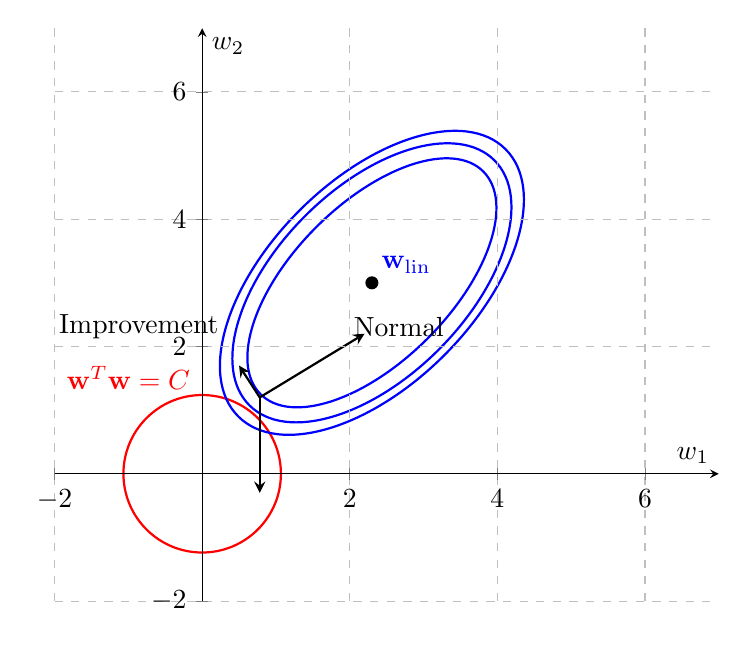
\begin{tikzpicture}
        \begin{axis}[
            xmin=-2, xmax=7,
            ymin=-2, ymax=7,
            axis lines=center,
            axis on top=true,
            ylabel=$w_2$,
            xlabel=$w_1$,
            domain=-3:6,
            grid=major,
            grid style=dashed,
            scale only axis,
        ]

        % Red circle for the constraint w^Tw = C
        \draw[style=thick, red] (axis cs:0,0) circle [radius=1cm];
        \node[red] at (axis cs:-1,1.5) {$\mathbf{w}^T\mathbf{w} = C$};

        % Blue ellipses for the ridge regression loss contours
        \draw[rotate around={-45:(axis cs:2.3,3)}, blue, thick] (axis cs:2.3,3) ellipse (1cm and 2.0cm);
        \draw[rotate around={-45:(axis cs:2.3,3)}, blue, thick] (axis cs:2.3,3) ellipse (1.2cm and 2.2cm);
        \draw[rotate around={-45:(axis cs:2.3,3)}, blue, thick] (axis cs:2.3,3) ellipse (1.3cm and 2.4cm);

        % Label for w_lin
        \node[anchor=south west, blue] at (axis cs:2.3,3) {$\mathbf{w}_{\text{lin}}$};
        % Point marker for w_lin
        \node[circle, scale=0.5, fill=black] at (axis cs:2.3,3) {};

        % Arrows
        \draw[-stealth, thick] (axis cs:0.78,1.2) -- (axis cs:0.5,1.7) node[pos=1.5, above left] {Improvement};
        \draw[-stealth, thick] (axis cs:0.78,1.2) -- (axis cs:0.78,-0.3);
        \draw[-stealth, thick] (axis cs:0.78,1.2) -- (axis cs:2.2,2.2) node[pos=0.8, above right] {Normal};

        \end{axis}
    \end{tikzpicture}
    \caption{Ridge regression visualisation}
    \label{fig:ridge-regress-viz}
\end{figure}


\begin{figure}[H]
    \centering
    \includegraphics[width=1\linewidth]{img/reg_legendre.png}
    \caption{Fitting Legendre polynomials to the objective function: setting $\lambda$ will affect the outcome of overfitting or underfitting.}
    \label{fig:reg-legendre}
\end{figure}

\subsubsection*{Choosing the Regularisation Parameter \( \lambda \)}
The choice of the regularisation parameter \( \lambda \) plays a critical role in the performance of the regularised model. It controls the trade-off between the fit of the model to the data and the magnitude of the coefficients:

\begin{itemize}
    \item A too-small \( \lambda \) may lead to overfitting, where the model captures noise in the training data.
    \item A too-large \( \lambda \) may lead to underfitting, where the model fails to capture the underlying trend in the data.
\end{itemize}

The value of \( \lambda \) is typically determined through cross-validation.

\subsection{Tikhonov Regularisation}

Tikhonov regularisation introduces a generalisation of the \( L_2 \) norm by allowing for the possibility of non-identity transformation matrices that can encode different types of prior knowledge about the weight coefficients. This general form is given as:

\begin{equation}
\|\mathbf{w}\|_{\Gamma}^2 = \mathbf{w}^T\Gamma^T\Gamma\mathbf{w},
\end{equation}
where \( \Gamma \) is a matrix that can incorporate information about the relationships between different features or can be used to impose specific structures on the solution.

\subsubsection*{Example of Tikhonov Regularisation}
A common choice for \( \Gamma \) is to use a diagonal matrix where the diagonal elements \( \gamma_q \) correspond to the inverse of the variance of each feature, normalising the features with respect to their scale. This choice of \( \Gamma \) leads to a standardised regularisation effect across all features.

\subsection{Lasso L1 Regularisation}

Lasso, which stands for Least Absolute Shrinkage and Selection Operator, is a regularisation technique that employs the \( L_1 \) norm of the weight vector:

\begin{equation}
\|\mathbf{w}\|_1 = \sum_{j=1}^{d} |w_j|,
\end{equation}
where \( d \) is the number of dimensions or features.

\subsubsection*{Lasso Formulation}
The Lasso problem to minimise empirical risk $\widehat{R})n$ can be formulated as:

\begin{definitionbox}{Lasso Problem}
    \begin{equation}
\min_{\mathbf{w}} \underbrace{\left\{ \frac{1}{n} \|\mathbf{Zw} - \mathbf{y}\|^2 \right\}}_{\widehat R_n=\frac1n(Z\mathbf{w}-\mathbf{y})^\top(Z\mathbf{w}-\mathbf{y})} \quad \text{subject to} \quad \|\mathbf{w}\|_1 \leq C,
\end{equation}
where \( C \) is a constant that controls the strength of the regularisation.
\end{definitionbox}



\begin{figure}[H]
    \centering
    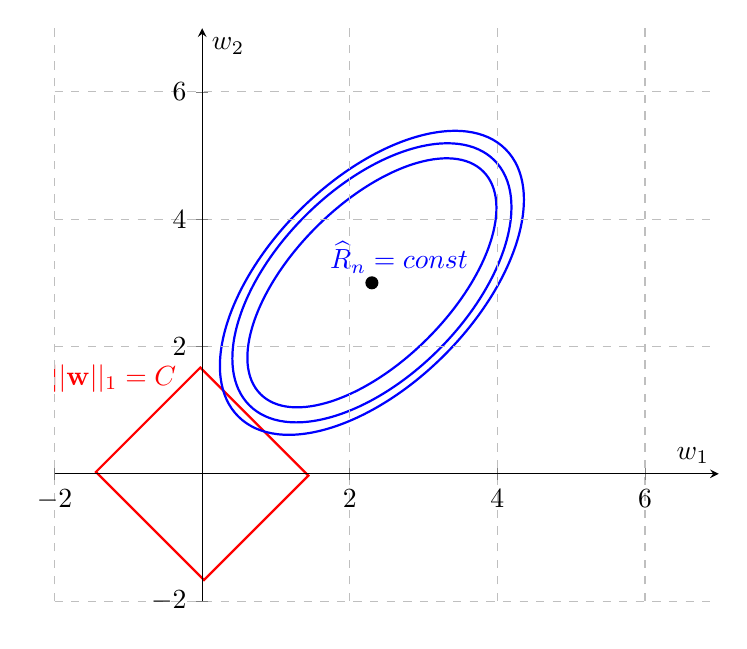
\begin{tikzpicture}
        \begin{axis}[
            xmin=-2, xmax=7,
            ymin=-2, ymax=7,
            axis lines=center,
            axis on top=true,
            ylabel=$w_2$,
            xlabel=$w_1$,
            domain=-3:6,
            grid=major,
            grid style=dashed,
            scale only axis,
        ]

        % Red circle for the constraint w^Tw = C
        \draw[style=thick, red, rotate around={45:(axis cs:0,0)}] (axis cs:-1,-1.2
        ) rectangle (axis cs:1,1.2);
        \node[red] at (axis cs:-1.2,1.5) {$||\mathbf{w}||_1 = C$};

        % Blue ellipses for the ridge regression loss contours
        \draw[rotate around={-45:(axis cs:2.3,3)}, blue, thick] (axis cs:2.3,3) ellipse (1cm and 2.0cm);
        \draw[rotate around={-45:(axis cs:2.3,3)}, blue, thick] (axis cs:2.3,3) ellipse (1.2cm and 2.2cm);
        \draw[rotate around={-45:(axis cs:2.3,3)}, blue, thick] (axis cs:2.3,3) ellipse (1.3cm and 2.4cm);

        % Label for R_n
        \node[anchor=south west, blue] at (axis cs:1.6,3) {$\widehat{R}_{n} = const$};
        % Point marker for w_lin
        \node[circle, scale=0.5, fill=black] at (axis cs:2.3,3) {};

        % Arrows
        % \draw[-stealth, thick] (axis cs:0.78,1.2) -- (axis cs:0.5,1.7) node[pos=1.5, above left] {Improvement};
        % \draw[-stealth, thick] (axis cs:0.78,1.2) -- (axis cs:0.78,-0.3);
        % \draw[-stealth, thick] (axis cs:0.78,1.2) -- (axis cs:2.2,2.2) node[pos=0.8, above right] {Normal};

        \end{axis}
    \end{tikzpicture}
    \caption{Lasso regression visualisation}
    \label{fig:lasso-regress-viz}
\end{figure}

\subsubsection*{Lasso Regularisation}
Lasso (Least Absolute Shrinkage and Selection Operator) employs \( L_1 \) penalty to achieve sparse solutions, effectively performing feature selection by constraining the sum of the absolute values of the model coefficients. This approach is beneficial in high-dimensional spaces where \( d \approx n \) or \( d > n \), as it reduces model complexity and prevents overfitting by enforcing some coefficients to shrink to zero. 


\begin{sidenotebox}{More information on the L1 Norms in Regularisation and why not the L0 Norm \\ }
\subsubsection*{The Problem}
We want to drop out features (components in the weight vector) that we don't need to make things sparse. So we want to minimise the number of non-zero weights in our weight vector.\\

Naively, we could start by constraining the $L_0$-Norm (mathematically, this isn't an actual norm):

\begin{equation*}
\|\mathbf{w}\|_0=\sum_{j=1}^d\mathbb{I}\left(\mathbf{w}_i\neq0\right)
\end{equation*}

Where $\mathbb{I}$ is the indicator function that returns 1 if the condition in its input is true, and 0 otherwise. So this is just the summation of all non-zero weights of the vector $\mathbf{w}$. However, this is a non-convex and NP-hard problem – there is no algorithm that can search through all possible subsets of features, this is a combinatorial search problem in $O(2^d)$ where $d$ is the number of features.\\

Instead, we set the constraint to be the $L_1$ norm of weights:

\[\|\mathbf{w}\|_1=\sum_{j=1}^d|\mathbf{w}_j|\]


Instead of going through all subsets of choosing weights or dropping them, we just set a  simpler limit on their absolute sum. This is a convex optimisation problem that can be solved more efficiently. In Figure \ref{fig:lasso-regress-viz}, note that the $L_1$ norm still is able to shrink coefficients exactly to zero, unlike the $L_2$ norm. This occurs because the optimisation function's contour lines are sharp around the axes where they intersect the elliptical contour of the empirical risk or loss function. At this point, we see that one coefficient on the axis is zero. All optimal values lie precisely on the axis. This is because the $L_1$ norm is shaped more like a diamond than a circle like in $L_2$ regularisation.\\

    However, the $L_1$ norm introduces some bias into the estimates, when true weights values are large. This happens because it shrinks all coefficients towards zero by the same absolute amount, not just the less significant ones – it does not consider true magnitude of each weight.\\
    
    Also, unlike it does not guarantee the selection of the correct subset of features all the time, especially when features are correlated.
\end{sidenotebox}

\subsubsection*{Mathematical Formulation}
The optimisation problem for Lasso is given by the Langrangian, combining the risk function as our objective, plus a multiple of the constraint:
\begin{equation}
\min_{\mathbf{w}} \left\{ \hat{R}_n(\mathbf{w}) + \lambda \|\mathbf{w}\|_1 \right\},
\end{equation}
where \( \hat{R}_n(\mathbf{w}) \) represents the empirical risk and \( \|\mathbf{w}\|_1 = \sum_{j=1}^{d} |\mathbf{w}_j| \) is the \( L_1 \) norm imposing sparsity. The parameter \( \lambda \) controls the degree of sparsity.

% \subsubsection*{Geometrical Insight}
% The \( L_1 \) norm's diamond contour interacts with the elliptical contours of the loss function, frequently intersecting at axes which correspond to sparser solutions. The intersection points represent feature selection through coefficient elimination.


% \subsubsection*{Lasso Constraint Selection}
% The key characteristic of Lasso regularisation is its ability to perform feature selection. The \( L_1 \) penalty has the property of forcing some coefficients to be exactly zero when the regularisation parameter \( \lambda \) is sufficiently large. This leads to models that are sparse with respect to the features used, providing an intrinsic method for feature selection.

% \subsubsection*{Sparse Solutions}
% The geometry of the \( L_1 \) penalty function makes it more likely that the optimisation path will hit the axes in the parameter space, which corresponds to a solution where some of the weights are exactly zero. This is illustrated in the contour plot where the elliptical contours of the loss function intersect with the diamond-shaped contours of the \( L_1 \) norm.

\subsubsection*{Sparse Models and Overfitting}
Sparse models are particularly useful in situations where the number of features \( d \) is close to or greater than the number of samples \( n \). By reducing the number of features, Lasso helps to mitigate the risk of overfitting, which can be a significant concern in high-dimensional datasets.


\subsubsection*{Benefits of LASSO Over Ridge}
LASSO has the advantage of producing sparse models, where some of the coefficients can become exactly zero, thereby performing feature selection:

\begin{itemize}
    \item This sparsity can be beneficial in high-dimensional datasets where it is desirable to reduce the number of features.
    \item It can lead to simpler models that are easier to interpret.
\end{itemize}

\begin{sidenotebox}{Elastic Net Regularisation}
Elastic Net is a compromise between ridge regression and LASSO, combining the \( L_2 \) penalty of ridge regression with the \( L_1 \) penalty of LASSO. It is useful when there are multiple features that are correlated with one another.

\begin{definitionbox}{Elastic Net Regularisation}
The regularisation term for Elastic Net is a linear combination of the \( L_1 \) and \( L_2 \) penalties:
\[
\lambda \left( \alpha \|\mathbf{w}\|_1 + \frac{1-\alpha}{2} \|\mathbf{w}\|_2^2 \right)
\]
where \( \alpha \) is the mixing parameter between \( L_1 \) penalty (LASSO) and \( L_2 \) penalty (ridge), typically chosen via cross-validation.
\end{definitionbox}

\subsubsection*{Algorithmic Implications}
The choice between ridge, LASSO, and Elastic Net also has algorithmic implications:

\begin{itemize}
    \item Ridge regression has a closed-form solution, which can be computed efficiently even for large datasets.
    \item LASSO and Elastic Net may require iterative methods to find a solution, which can be computationally more intensive.
\end{itemize}

The computational complexity should be considered when choosing the regularisation method, especially for large-scale applications.

\subsubsection*{Regularisation in Non-Linear Models}
While regularisation is commonly discussed in the context of linear models, it is equally applicable to non-linear models:

\begin{itemize}
    \item In kernel methods, regularisation controls the complexity of the model in the high-dimensional feature space induced by the kernel.
    \item In neural networks, regularisation can take various forms, including weight decay (similar to \( L_2 \) regularisation) and dropout (a form of stochastic regularisation).
\end{itemize}
\end{sidenotebox}

\subsection{Tikhonov Regularisation}

Tikhonov regularisation is applied in the context of machine learning to prevent overfitting and to improve the generalisation of the model. It does this by adding a regularisation term to the loss function, which penalises complex models:

\begin{itemize}
    \item The loss function with Tikhonov regularisation is given by:
    \[
    \mathcal{L}_n(\mathbf{w}) = \hat{R}_n(\mathbf{w}) + \lambda \|\mathbf{w}\|_Q^2,
    \]
    where \( \hat{R}_n(\mathbf{w}) \) is the empirical risk, \( \lambda \) is the regularisation parameter, and \( \|\mathbf{w}\|_Q^2 \) is the Tikhonov regulariser.
    
    \item The Tikhonov regulariser can be expressed as a weighted sum of the squared weights:
    \[
    \|\mathbf{w}\|_Q^2 = \sum_{q=0}^{Q} \gamma_q w_q^2,
    \]
    where \( \gamma_q \) are the weights that can be adjusted to control the regularisation of the corresponding parameters \( w_q \).

    \item The regularisation term places emphasis on certain weights, which can be tuned according to the desired complexity of the model:
    \begin{itemize}
        \item For a low-order fit, which favours simplicity, the weights \( \gamma_q \) can be chosen as \( \gamma_q = 2^q \).
        \item For a high-order fit, which allows for more complexity, the weights \( \gamma_q \) can be chosen as \( \gamma_q = 2^{-q} \).
    \end{itemize}
\end{itemize}

Tikhonov regularisation introduces a generalisation of the \( L_2 \) norm by allowing for the possibility of non-identity transformation matrices that can encode different types of prior knowledge about the weight coefficients. This general form is given as:



\begin{equation}
\|\mathbf{w}\|_{Q}^2 = \mathbf{w}^T\Gamma^T\Gamma\mathbf{w} \quad Q = \Gamma^\top\Gamma,
\end{equation}
where \( \Gamma \) is a matrix that can incorporate information about the relationships between different features or can be used to impose specific structures on the solution.

\subsubsection*{Example of Tikhonov Regularisation}
A common choice for \( \Gamma \) is to use a diagonal matrix where the diagonal elements \( \gamma_q \) correspond to the inverse of the variance of each feature, normalising the features with respect to their scale. This choice of \( \Gamma \) leads to a standardised regularisation effect across all features.




\section{The Need for Validation}
\subsection*{Example Problem}
\begin{figure}[H]
    \centering\includegraphics[width=0.75\linewidth]{img/choose_lambda.png}
    \caption{If we have too much deterministic and stochastic noise, this increases our chance of overfitting. Increasing the number of data points and our regularisation coefficient $\lambda$ helps to combat this.}
    \label{fig:enter-label}
\end{figure}

\subsection*{Regularised Loss Function}
The regularised loss, denoted as \( L_n(h) \), combines the empirical risk \( \hat{R}(h) \) with a regularisation term \( \Omega(h) \), scaled by a factor \( \lambda \):
\begin{equation}
  L_n(h) = \hat{R}(h) + \lambda \underbrace{\Omega(h)}_{\text{overfit penalty (regularisation)}}
\end{equation}
where \( \lambda \) is the regularisation coefficient controlling the trade-off between the empirical risk and the penalty term.\\

Note the similarity in structure to the Vapnik-Chervonenkis (VC) inequality provides a theoretical bound on the model's generalisation error:
\begin{equation}
  R(h) \leq \hat{R}(h) + \underbrace{\Omega(n, H, \delta)}_{\text{complexity penalty}}
\end{equation}
where \( \Omega(n, H, \sigma) \) represents the complexity penalty associated with the hypothesis space \( H \), the sample size \( n \), and the variance \( \sigma \) of the noise in the data.\\

In essence, we ideally want to minimise the true risk $R(h)$. However, due to limited knowledge, data, noise, true distribution, etc, we cannot compute true risk directly.\\

In earlier section \ref{vc-ineq-subsection} we learnt the VC inequality provides a theoretical upper bound on the true risk based on empirical risk plus a complexity term that depends on the number of data samples $n$, capacity of hypothesis space $\mathcal{H}$, and confidence level $\delta$. \\

In regularisation, we add a penalty term $\Omega (h)$ as an attempt to approximate the complexity term in the VC inequality, by penalising the model complexity we ensure we do not overfit to training data, which is aligned with the goal of VC inequality to control true risk.\\

\begin{commentbox}{Note to Self}
    \textbf{NOTE: the module slides says that $\mathcal{L}_n(h)$ approximates true risk better than the VC inequality, this needs further checking.}
\end{commentbox}


\subsection*{Types of Regularisers}
Various regularisation techniques are used to control different aspects of model complexity:
\begin{itemize}
  \item Ridge Regression: \( \|\mathbf{w}\|_2^2 \) penalises the square of the coefficients, favouring smaller, more diffuse weight values.
  \item Lasso: \( \|\mathbf{w}\|_1 \) encourages sparsity in the model's coefficients, leading to feature selection.
  \item Elastic Net: \( \|\mathbf{w}\|_1 + \|\mathbf{w}\|_2^2 \) combines the penalties of ridge regression and lasso, balancing between feature selection and coefficient shrinkage.
  \item Tikhonov Regularisation: \( \mathbf{w}^T\mathbf{Q}\mathbf{w} \) allows incorporation of prior knowledge through matrix \( \mathbf{Q} = \Gamma^\top \Gamma \) where $\Gamma$ is a matrix of weights.
\end{itemize}


\subsection*{Occam's Razor and Regularisation}
Occam's razor posits that simpler explanations are generally preferable, so in machine learning, we tend to choose simpler models when regularising.\\

This is because noise, which is inherently present in data, is not smooth or structured; therefore, a smoother function, less likely to capture noise, is more desirable.
Validation is a critical process in the development of a machine learning model. It allows for the evaluation of the model's performance on an independent data set, known as the validation set. The following steps outline the validation process in both specific and general contexts, incorporating regularization, hypothesis classes, and the selection of hyperparameters.

\section{Validation}
Regularisation involves adding an overfit penalty to the empirical risk, to determine the final performance.
\[\mathcal{L}_n(h)=\widehat{R}_n(h)+\lambda\underbrace{\Omega(h)}_{\text{overfit penalty}}\]

Validation is attempt to directly estimate the performance by training the model on a portion of the dataset and using another unseen portion of data to gauge its performance.
\[\underbrace{\mathcal{L}_n(h)}_{\text{direct estimation}}=\widehat{R}_n(h)+\lambda\underbrace{\Omega(h)}_{\text{overfit penalty}}\]

\subsection*{Validation Process}
In this section, $n$ refers to the size of the whole dataset and $v$ refers to the size of the validation dataset.
\begin{enumerate}
  \item Split the training data \( D \) into training \( D_{\text{train}} \) and validation \( D_{\text{val}} \) sets.
  \item Train the model \( g \) on \( D_{\text{train}} \).
  \item Estimate its performance on \( D_{\text{val}} \) with \( v = |D_{\text{val}}| \):
  \begin{equation}
    \check{R}_{v}(g) = \frac{1}{v} \sum_{(x,y) \in D_{\text{val}}} \ell(g(x), y)
  \end{equation}
  where \( \ell(g(x), y) \) is the loss function evaluating the prediction \( g(x) \) against the true output \( y \).
  \item Utilise the validation set to provide an unbiased estimate of the true risk \( R(g) \), which, under certain conditions, is very close to the expected risk calculated through validation \[\mathbb{E}_{\mathcal{D}_{\mathrm{val}}}\left[\check{R}_{\nu}(\mathbf{g})\right]\approx R(\mathbf{g})\leqslant\quad\check{R}_{\nu}(\mathbf{g})+\underbrace{\Omega(\mathbf{v},\mathbf{\delta})}_{\sim\sqrt{\log(1/\delta)/v}\leftarrow\text{one model only on }\mathbf{v}-\mathrm{points}} \text{with probability }1-\delta \]
\end{enumerate}

The validation dataset \( D_{\text{val}} \) is unbiased, with a small Hoeffding bound, and only one hypothesis \( g \) is considered.
Select \( \lambda^* \) as the argument that minimises the regularised risk \( \hat{R}_{\lambda}(g) \),
\begin{equation*}
    \lambda^* = \underset{\lambda}{\mathrm{argmin}} \, \hat{R}_{\lambda}(g),
\end{equation*}
then train on the whole dataset \( D \) with \( \lambda^* \).


\subsection*{Validation More Generally}

\begin{enumerate}
  \item Given hypothesis classes \( (\mathcal{H}_1, \lambda_1), \ldots, (\mathcal{H}_m, \lambda_m) \), split \( D \) into \( D_{\text{train}} \) and \( D_{\text{val}} \).
  \item Train \( g_i \) on \( D_{\text{train}} \) with \( |D_{\text{train}}| = n - v \), where $n$ is the size of the whole dataset and $v$ is the size of the validation dataset.
  \item Select \( i_* \) such that \( g_i* = \arg\min_{g_i} \hat{R}_{\text{v}}(g_i) \) on \( |D_{\text{val}}| = v \), where \( i \) can represent not only regularisation but also other hyperparameters.
  \item Select \( \mathcal{H}_i, \lambda_i \) and train new \( g \) on \( D_{\text{val}} \cup D_{\text{train}} \) to get the final \( g^* \).
\end{enumerate}

\begin{figure}[H]
    \centering
    \includegraphics[width=0.75\linewidth]{img/validation.png}
    \caption{Credit: Caltech ML Lectures}
    
\end{figure}


Note that as you increase your validation set size, you will end up picking a hypothesis that best matches the actual true risk for that hypothesis $R(h)$ (denoted as $E_{out}$), however, this error is expected to be higher, a compromise that comes with shrinking the training set size because you increased the validation set size.

\begin{figure}[H]
    \centering
    \includegraphics[width=0.5\linewidth]{img/bias_validation.png}
    \caption{Credit: Caltech ML Lectures}
    
\end{figure}

\subsection*{Discussion and Considerations}

\begin{itemize}
  \item The choice of \( v \) influences the bias-variance trade-off. A small \( v \) may lead to an underestimate of the true risk, while a large \( v \) may increase the variance of the risk estimate.
  \item The size of \( D_{\text{val}} \) is often set to \( \frac{|D|}{5} \) as a rule of thumb, balancing the need for a representative validation set against the need to retain sufficient training data.
  \item Note: the terminology here calls this the "validation set" as opposed to "test set", to emphasise the iterative nature of model selection, which may involve multiple rounds of training and validation before a final test on an unseen data set.
\end{itemize}

\subsection{K-Fold Cross-Validation}
\begin{figure}[H]
    \centering
    \includegraphics[width=0.5\linewidth]{img/crossv.png}
    \caption{Cross Validation illustrated, the red cells refer to the validation subsets}
    \label{fig:crossv}
    % \caption{Enter Caption}
    
\end{figure}
K-fold cross-validation is a model validation technique to assess the predictive performance of a machine learning model. It helps ensure that the model's performance is independent of the way we partition the data into training and test sets.\\

This involves fitting and evaluating $K$ models, training on a (usually larger) set of data and validating on a (usually smaller) portion of unseen data, as seen in Figure \ref{fig:crossv}

\subsection*{Procedure}
Given a dataset $\mathcal{D}$ and a hypothesis class $\mathcal{H}$ with hyperparameter $\theta$, the K-fold cross-validation process is as follows:

\begin{enumerate}
    \item Partition the dataset $\mathcal{D}$ into $K$ distinct subsets $\mathcal{D}_1, \mathcal{D}_2, \ldots, \mathcal{D}_K$ of equal size. Each subset $\mathcal{D}_k$ serves as a validation set, and the remaining $K-1$ subsets are used as the training set.
    
    \item For each hypothesis $(\mathcal{H}_i, \theta_i)$ in the hypothesis classes $(\mathcal{H}_1,\theta_1),(\mathcal{H}_2,\theta_2),\ldots,(\mathcal{H}_M,\theta_M)$, repeat the following steps:
    \begin{enumerate}
        \item Train a model $g_i$ using empirical risk minimization (ERM) on the training set excluding $\mathcal{D}_k$.
        \item Evaluate the validation error $R_{\mathcal{V}}(g_i)$ of the model $g_i$ on the validation set $\mathcal{D}_k$.
        \item Select the model $g_{i^*} = \arg\min_{g_i} R_{\mathcal{V}}(g_i)$ with the lowest validation error.
    \end{enumerate}
    
    \item After training and evaluating on all $K$ folds, use the hypothesis $(\mathcal{H}_{i^*}, \theta_{i^*})$ and the entire dataset $\mathcal{D}$ to train the final model $g^*$.
\end{enumerate}

Example: If you use $K=3$, you would find the best model $g$ that is trained on subset 1 and 2 and validated on 3. Then find the best model trained on 2, validated on 1 and 3. Then find the best model trained on 3, validated on 1 and 2.Then take the average of the cross-validation error for all three cases, this will be an estimate for expected generalisation error.

\subsection*{Mathematics of K-fold Cross Validation}
The validation error $R_k(g_{i_k})$ for each fold $k$ is calculated as:
\begin{equation}
\check{R}_k(g_{\bar{k}})=\frac{1}{|\mathcal{D}_k|}\sum_{(\mathbf{x}_i,\mathbf{y}_i)\in\mathcal{D}_k}\ell(g_{\bar{k}}(\mathbf{x}_i),y_i)\quad \text{ with }\bar{n}=(K-1/K)n
\end{equation}
where $\ell$ is the loss function, $(x_i, y_i)$ are the data points in the validation set $\mathcal{D}_k$, and $|\mathcal{D}_k|$ is the size of the validation set.

The cross-validation error $R_{\text{CV}}$ is the average of the validation errors over all $K$ folds:
\begin{equation}
R_{\text{CV}} = \frac{1}{K} \sum_{k=1}^{K} R_k(g_{i_k})
\end{equation}

The expected cross-validation error is an unbiased estimate of the expected generalisation error:
\begin{equation}
\mathbb{E}_{\mathcal{D}} [R_{\text{CV}}] = \mathbb{E}_{\mathcal{D}} [R(g_{i_k})]
\end{equation}

\subsection*{Typical Choices for \textit{K}}
\begin{itemize}
    \item $K = 10$: This is the standard choice for 10-fold cross-validation.
    \item $K = n$: Known as leave-one-out cross-validation, where $n$ is the number of data points in the dataset $\mathcal{D}$ This is usually done when there is a small dataset and the model is not too computationally expensive, because this requires a lot of training iterations, creating and evaluating one model for each example in the dataset.
\end{itemize}

\section{Revisiting The SRM}

We have covered Structural Risk Minimisation and Validation previously in \ref{SRM-section}:

\begin{definitionbox}{Structural Risk Minimisation}


From the generalisation bound of the VC Inequality in
\[R(h) \leq \widehat{R}_n(h) + \sqrt{\frac{8d_{VC}(\mathcal{H})}{n} \log\left(\frac{2n + 1}{\delta}\right) + \frac{8}{n} \log\frac{4}{\delta}}\\\]

We have with probability of at least $1-{\color{red} w_i}\delta$, for all $h \in \mathcal{H}_i$:
    \begin{align*}
R(h) &\leq \widehat{R}_n(h) + \sqrt{\frac{8d_{VC}(\mathcal{H})}{n} \log\left(\frac{2n + 1}{\delta}\right) + \frac{8}{n} \log\frac{4}{w_i\delta}}\\
R(h) &\leq \widehat{R}_n(h) + \Omega(n, \mathcal{H}_i, {\color{red} w_i}\delta)    
    \end{align*}
SRM Solution: 
    \[g = \text{argmin}_{h \in \mathcal{H}}\widehat{R}_n(h) + \Omega(n, \mathcal{H}(h), {\color{red} w_i}\delta)\]

    \begin{itemize}
        \item $\mathcal{H}(h)$ is the simplest class $h$ belongs to, and $w_i$ is the class weight.
        \item Training error $\hat{R}_n(h)$ plus complexity term $\Omega$ (from VC inequality).
        \item Identical to ERM if there is only one class $\mathcal{H}$.
    \end{itemize}

    \end{definitionbox}

    \begin{definitionbox}{Generalisation Bound}
        We then have, with probability of at least $1-\delta$,

        \begin{align*}
R(\mathbf{g})& \leqslant\min_{i}\left(R(h_{i}^{*})+2\Omega(n,{\mathcal H}_{i},w_{i}\delta)\right)  \\
&\leqslant R(h^*)+2\Omega(n,\mathcal{H}(h^*),w(h^*)\delta)
\end{align*}

Where $h^*_i = \text{argmin}_{h\in\mathcal{H}_i}R(h_i)$ and $h^* = \text{argmin}_{h\in\mathcal{H}}R(h)$.\\

This means that our risk for our hypothesis $g$ determined by SRM (which factors in for regularisation penalities) is bounded by the true risk plus the VC inequality complexity penalty for that given hypothesis class.

\subsubsection*{Proof:}
Let $\Omega_h = \Omega(n, \mathcal{H}(h), w(h)\delta)$. Then with probability of at least $1-\delta$ for any $h \in \mathcal{H}:$
\[R(g)-R(h)=\underbrace{R(g)-(\hat{R}_n(g)+\Omega_g)}_{\leqslant0\text{ (VC inequality)}}+\underbrace{(\hat{R}_n(g)+\Omega_g)-(\hat{R}_n(h)+\Omega_h)}_{\leqslant0\text{ by def. of g}}+{\color{red}\Omega_h}+\underbrace{\hat{R}_n(h)-R(h)}_{\leqslant{\color{red}\Omega_h}\text{ (VC inequality)}}\]
    \end{definitionbox}

\subsection*{Hypothesis Space and Preferences}
The hypothesis space \( \mathcal{H} \) is structured as a union of nested classes \( \mathcal{H}_i \), each with an associated complexity and preference weight \( w_i \), with \( \sum w_i = 1 \).

\subsection*{Choosing Weights}
The selection of weights \( w_i \) influences the trade-off between model complexity and fit to the data, akin to selecting a regularization parameter in practical applications. No preference implies equal weighting ($w_i = 1/N$) for $N$ classes, whereas a preference for simplicity implies higher weights for simpler models.


\begin{figure}[H]
    \centering
\includegraphics[width=1\linewidth]{img/RLM.png}
\includegraphics[width=0.75\linewidth]{img/srm-2side.png}    
\includegraphics[width=0.75\linewidth]{img/srm2.png}
\end{figure}

\begin{figure}[H]
    \centering
\includegraphics[width=0.55\linewidth]{img/terminology_3.png}

\end{figure}

\section{Approaching a Practical Machine Learning Problem}

\begin{enumerate}
    \item Take the problem and translate its details into a machine learning problem.
    \begin{itemize}
        \item Identify what kind of task it is, classification, regression, etc.
        \item Convert input data into a vector representation \textbf{x}
        \item Utilise an error or loss function $\ell(h(x),y)$ based on the application.
        \item Select hypothess classes $\mathcal{H}$ with their learning algorithms
    \end{itemize}
    \item Follow one of the know methods: ERM, SRM, Regularisation, Validation
    \item Plan and execute experiments
    \item Present and analyse the results
\end{enumerate}

\chapter{Optimisation and Learning}
\section{Logistic Regression}
\subsection{Maximum Likelihood Predictor}
Maximum likelihood estimation is a method to estimate the parameters of a statistical model, which in the context of logistic regression, leads to finding the best coefficients for the predictors.\\

\textbf{1. Statistical Model Setup:}
\begin{itemize}
    \item We have a binary class \( y \) representing two possible outcomes, with \( y = +1 \) and for the event's occurrence and \(y=-1\) for it not occurring.
    \item Distribution \( P(y) \) for the class variable \( y \).
    \item Observations \( x_1, x_2, \ldots, x_d \) are independent binary features 0 or 1 that contribute to the prediction of $y$.
    \item Note that $x \in \{0,1\}$ and $y \in \{-1,1\}$
\end{itemize}

\textbf{2. Assumptions:}
\begin{itemize}
    \item We assume each feature $x_i$ is independent, and so:
    \[ P(x_1, \ldots, x_d|y) = P(x_1|y) \times \ldots \times P(x_d|y) \]
\end{itemize}

\textbf{3. Posterior Probability:}
\begin{itemize}
    \item With Bayes' rule, we have:
    \[ P(y|x_1, \ldots, x_d) = \frac{P(y) \times P(x_1, \ldots, x_d|y)}{P(x_1, \ldots, x_d)} \]
    \item Assuming feature independence:
    \[ P(y|x_1, \ldots, x_d) = \frac{P(y) \times \prod_{i=1}^{d} P(x_i|y)}{P(x_1, \ldots, x_d)} \]
\end{itemize}

\textbf{4. Odds and Log Odds:}
\begin{itemize}
    \item The odds of $y$ being 1 or -1 is the ratio of their respective probabilities. By independence, this the product of every feature's probability given y:
    \begin{align*}\frac{P(y=1|x_1,\ldots,x_d)}{P(y=-1|x_1,\ldots,x_d)}&=\frac{P(x_1|y=1)}{P(x_1|y=-1)}\times\ldots\times\frac{P(x_d|y=1)}{P(x_d|y=-1)}\times\frac{P(y=1)}{P(y=-1)}\end{align*}

    Taking the log of the odds make everything more mathematically convenient, and we see this starts to look like a linear model:
    \begin{align*}
    \log\frac{P(y=1|x_1,\ldots,x_d)}{P(y=-1|x_1,\ldots,x_d)}&=\log\frac{P(y=1)}{P(y=-1)}+\sum_{i=1}^{d}\log\frac{P(x_i|y=1)}{P(x_i|y=-1)}\\
&=w_0+ \sum_{i=1}^dw_i^*\mathbf{x}_i=\mathbf{w}_*^\top\mathbf{x}
    \end{align*}

As part of the training/learning process, we want to consider $P(x_i|y)$, which is the probability of our observations of the data, given a label $y$.
Since $x$ can only take on two values, we can specify $P(x_i|y)$ as a piecewise function:
\[
P(x_i|y)=
\begin{cases}
    P(x_i = 1 | y) & \text{if } x_i = 1 \\
P(x_i = 0 | y) & \text{if } x_i = 0
\end{cases} \]

When we take the logarithm of \( P(x_i | y) \), we are just applying the logarithm function to the above piecewise definition. However, we want a single equation that works for both cases (when \( x_i = 1 \) and \( x_i = 0 \)). To achieve this, we use \( x_i \) itself as a coefficient that becomes 1 when \( x_i = 1 \) and 0 when \( x_i = 0 \), and similarly, \( (1 - x_i) \) becomes 0 when \( x_i = 1 \) and 1 when \( x_i = 0 \).
Now, let's derive the equation:
For \( x_i = 1 \), the log probability is:
\[ \log P(x_i | y) = \log P(x_i = 1 | y) \]
For \( x_i = 0 \), the log probability is:
\[ \log P(x_i | y) = \log P(x_i = 0 | y) \]
Since \( x_i \) can only be 0 or 1, we can write the log probability as a single expression that accounts for both cases by using \( x_i \) and \( 1 - x_i \) as weights:
\[ \log P(x_i | y) = x_i \log P(x_i = 1 | y) + (1 - x_i) \log P(x_i = 0 | y) \]
What this does is select the correct log probability term based on the value of \( x_i \), `turning on' the first case and `turning off' the second case when $x_i = 1$, and vice versa when $x_i = 0$.

Expanding further, we get:
\begin{align*}
\log P(x_{i}|y)& =x_i\log P(x_i=1|y)+(1-x_i)\log P(x_i=0|y)  \\
&=x_{i}\bigg(\underbrace{\log P(x_{i}=1|y)-\log P(x_{i}=0|y)}_{\beta_{i,y} \text{ that depends on observation } x_i \in \{0,1\} \text{from the data}}\bigg)+\underbrace{\log P(x_{i}=0|y)}_{\gamma_{i,y} \text{ always added regardless of observation $x_i$}}\\
&= x_i(\beta_{i,y}) + \gamma_{i,y} \\
\text{where }& \beta_{i,y} = \log P(x_{i}=1|y)-\log P(x_{i}=0|y)\\
& \gamma_{i,y}=\log P(x_{i}=0|y)
\end{align*}

We use $\beta_{i,y}, \gamma_{i,y}$ to refer to parameters that are estimated from our data. \\

Going back to our log likelihood estimator and plugging in our values:

\begin{align*}
\log{\frac{P(x_{i}|y=1)}{P(x_{i}|y=-1)}}& =\log P(x_i|y=1)-\log P(x_i|y=-1)  \\
&= (x_i(\beta_{i,y=1}) + \gamma_{i, y=1}) - (x_i(\beta_{i,y=-1}) + \gamma_{i, y=-1})\\
&=x_{i}(\underbrace{\beta_{i,1}-\beta_{i,-1}}_{w_{i}^{*}})+\underbrace{(\gamma_{i,1}-\gamma_{i,-1})}_{w_0^*}
\end{align*}

We see this is very similar to a linear prediction model.
\end{itemize}

\textbf{5. Logistic Regression Model:}
\begin{itemize}
    \item Maximising the likelihood of the observed data through log-likelihood.
    \item We also relax binary and independence assumptions on $x_i$, so we can use numbers as more descriptive data features.\\

    With x=$(1,x_1,\ldots,x_d)$ and $y\in(-1,+1\}$, assume: 
    \begin{align*}&\log\frac{P(y=+1|x_1,\ldots,x_d)}{P(y=-1|x_1,\ldots,x_d)}=\mathbf{w}_*^\top\mathbf{x}=h(\mathbf{x},\mathbf{w})\end{align*}
    Using $P(y=-1|\mathbf{x})=P(y=-1|x_1,\ldots,x_d)=1-P(y=+1|x_1,\ldots,x_d)$, we have
    
    \begin{align*}
P(y=+1|\mathbf{x})&=\theta(\mathbf{w}_*^\top\mathbf{x})\\
    P(y=-1|\mathbf{x})&=1-\theta(\mathbf{w}_*^\top\mathbf{x})
    \end{align*}

    We get our logistic function
    \[P(y=1|\mathbf{x})=\frac{e^{\mathbf{w}_*^\top\mathbf{x}}}{1+e^{\mathbf{w}_*^\top\mathbf{x}}}=\frac1{1+e^{-\mathbf{w}_*^\top\mathbf{x}}}=\theta(\mathbf{w}_*^\top\mathbf{x})\]
    
We use $\mathbf{w}_*$ to refer to the set of weights that minimises the empirical error, the true and most accurate weight.
    
\end{itemize}
\begin{figure}[H]
    \centering
    \includegraphics[width=0.75\linewidth]{img/sigmoid.png}
    \caption{Sigmoid function}
    \label{fig:sigmoid-label}
\end{figure}
\subsection{Model Probabilities}
The probability of the outcome \( y \) given a predictor \( \mathbf{x} \) is modeled as:

\[
P(y|\mathbf{x}) = 
\begin{cases}
\theta(\mathbf{w}^\top\mathbf{x}) & \text{if } y = +1;\\
1 - \theta(\mathbf{w}^\top\mathbf{x}) & \text{if } y = -1,
\end{cases}
\]

where:
\begin{itemize}
    \item \( \theta(s) \) is the logistic function defined as \( \theta(s) = \frac{1}{1 + e^{-s}} \).
    \item \( \mathbf{w} \) is the weight vector.
    \item \( \mathbf{w}^\top\mathbf{x} \) is the dot product of the weight vector and the feature vector.
\end{itemize}

\subsubsection*{Likelihood Function}
The likelihood of an observed dataset \( D = \{(\mathbf{x}_1, y_1), \ldots, (\mathbf{x}_n, y_n)\} \) under the logistic regression model is given by the product of individual probabilities:

\[
L(\mathbf{w}) = \prod_{i=1}^{n} P(y_i|\mathbf{x}_i) = \prod_{i=1}^{n} \theta(y_i\mathbf{w}^\top\mathbf{x}_i).
\]

\subsubsection*{Log-Likelihood}
The log-likelihood, which transforms the product into a sum, making it computationally more convenient, is:

\[
\log L(\mathbf{w}) = \sum_{i=1}^{n} \log \theta(y_i\mathbf{w}^\top\mathbf{x}_i).
\]

To facilitate gradient-based optimisation, we minimise the negative of the log-likelihood:

\[
-\log L(\mathbf{w}) = -\sum_{i=1}^{n} \log \theta(y_i\mathbf{w}^\top\mathbf{x}_i) = \sum_{i=1}^{n} \log \left(1 + e^{-y_i\mathbf{w}^\top\mathbf{x}_i}\right).
\]

\subsection{Cross-Entropy Error}
The negative log-likelihood is equivalent to the cross-entropy error, which is commonly used as the error measure in logistic regression:

\[
\hat{R}_n(\mathbf{w}) = \frac{1}{n} \sum_{i=1}^{n} \log \left(1 + e^{-y_i\mathbf{w}^\top\mathbf{x}_i}\right).
\]

This cross-entropy error function is convex, and its minimisation leads to the maximum likelihood estimation of the model parameters \( \mathbf{w} \).

In logistic regression, the predicted probability for a positive class is modelled by the logistic function \( h(\mathbf{x}) \), defined as:
\[ h(\mathbf{x}) = \sigma(\mathbf{w}^\top \mathbf{x}) = \frac{1}{1 + e^{-\mathbf{w}^\top \mathbf{x}}} \]
The loss function, derived from the negative log-likelihood for the Bernoulli distribution, is given by:
\[ \ell(h(\mathbf{x}), y) = \begin{cases}
\log \frac{1}{h(\mathbf{x})} & \text{if } y = +1;\\
\log \frac{1}{1 - h(\mathbf{x})} & \text{if } y = -1.
\end{cases} \]
The cross-entropy error over a dataset is the average loss:
\[ \hat{R}_n = \frac{1}{n} \sum_{i=1}^{n} \left[ \mathbb{I}(y_i = +1) \log \frac{1}{h(\mathbf{x}_i)} + \mathbb{I}(y_i = -1) \log \frac{1}{1 - h(\mathbf{x}_i)} \right] \] where $\mathbb{I}$ is the indicator function that returns 1 when its argument evaluates to true, and -1 when false.
Considering entropy and cross-entropy:
\begin{itemize}
\item Entropy \( H(p) \) is:
\[ H(p) = p \log \frac{1}{p} + (1 - p) \log \frac{1}{1 - p} \]
\item Cross-entropy \( H(p, q) \) between two distributions \( p \) and \( q \) is:
\[ H(p, q) = p \log \frac{1}{q} + (1 - p) \log \frac{1}{1 - q} \]
\end{itemize}
Minimizing the cross-entropy error function during training optimises the weight vector \( \mathbf{w} \) to improve the predictive accuracy of the logistic regression model.


\subsection{Empirical Risk Minimisation for Logistic Regression}

The formula for empirical risk from linear regression is \[
\widehat R_n(\mathbf{w})=\frac1n\sum_{i=1}^n(y_i-\mathbf{w}^\top\mathbf{x}_i)^2
\] 

this is a convex problem that has a closed-form solution.\\

For logistic regression, however, we have 
\[
\widehat R_n(\mathbf{w})=\frac1n\sum_{i=1}^n\log\left(1+e^{-y_i\mathbf{w}^\top\mathbf{x}_i}\right);
\]

Which has no closed form solution. We require gradient descent.

\section{Gradient Descent}

Gradient descent is a widely-used optimization algorithm in machine learning, specifically for training logistic regression models. It iteratively adjusts model parameters to minimize the cost function, typically the cross-entropy loss.

\subsection{Direction of Descent}
The parameter update rule in gradient descent is given by:
\[ \mathbf{w}_{t+1} = \mathbf{w}_t + \eta\mathbf{v}, \]
where \( \mathbf{v} \) is the direction vector of the steepest descent, and \( \eta \) represents the learning rate.

\subsection{Step Size in Gradient Descent}
The learning rate \( \eta \) is crucial for the convergence of gradient descent:
\begin{itemize}
    \item A small \( \eta \) may slow down convergence.
    \item An overly large \( \eta \) can cause divergence.
    \item An adaptive \( \eta \) can improve convergence speed and stability.
\end{itemize}



\begin{sidenotebox}{More information on gradient descent}
If $\mathbf{v}=-\frac{\nabla\hat{R}_{n}(\mathbf{w}_{t})}{\|\nabla\hat{R}_{n}(\mathbf{w}_{t})\|}$, direction is defined by:
\begin{align*}\Delta\hat{R}_{n}&=\hat{R}_{n}(\mathbf{w}_{t+1})-\hat{R}_{n}(\mathbf{w}_{t})\\
&=\hat{R}_{n}(\mathbf{w}_{t}+\eta\mathbf{v})-\hat{R}_{n}(\mathbf{w}_{t})\\
&=\eta\nabla\hat{R}_{n}(\mathbf{w}_{t})^{\top}\mathbf{v}+O(\eta^{2})\geqslant-\eta\|\nabla\hat{R}_{n}(\mathbf{w}_{t})\|+O(\eta^{2})\end{align*}

The direction of the parameter update in gradient descent is key to effectively minimising the risk function \( \hat{R}_n \). The change in \( \hat{R}_n \) after an update is defined as:

\[ \Delta \hat{R}_n = \hat{R}_n(\mathbf{w}_{t+1}) - \hat{R}_n(\mathbf{w}_t) \]

Given the update rule \( \mathbf{w}_{t+1} = \mathbf{w}_t + \eta\mathbf{v} \), where \( \mathbf{v} \) is a unit vector and \( \eta \) is the learning rate, we can approximate the change in \( \hat{R}_n \) using a Taylor expansion:

\[ \hat{R}_n(\mathbf{w}_{t+1}) \approx \hat{R}_n(\mathbf{w}_t) + \eta \nabla \hat{R}_n(\mathbf{w}_t)^\top \mathbf{v} + O(\eta^2) \]

The optimal direction \( \mathbf{v} \) for the steepest descent is in the direction of the negative gradient, normalised:

\[ \mathbf{v} = -\frac{\nabla \hat{R}_n(\mathbf{w}_t)}{\| \nabla \hat{R}_n(\mathbf{w}_t) \|} \]

Incorporating this into the update rule, we achieve the gradient descent step:

\[ \mathbf{w}_{t+1} = \mathbf{w}_t - \eta \frac{\nabla \hat{R}_n(\mathbf{w}_t)}{\| \nabla \hat{R}_n(\mathbf{w}_t) \|} \]

This step ensures that the parameters are updated in the direction that most rapidly decreases the risk function \( \hat{R}_n \), taking into account the magnitude of the learning rate \( \eta \).
\end{sidenotebox}



\subsection{Empirical Risk Minimisation (ERM)}
In the context of logistic regression, ERM aims to find the optimal parameter vector \( \mathbf{w}^* \) by minimising the empirical risk \( \hat{R}_n(\mathbf{w}) \), the average loss over the dataset.


\begin{definitionbox}{Gradient Descent Algorithm}
\begin{itemize}
    \item Initialise the weight vector \( \mathbf{w}_0 \).
    \item For each iteration \( t \):
    \begin{enumerate}
        \item Compute the gradient of \( \hat{R}_n \) or \( \mathcal{L}_n \):
        \[ \nabla\hat{R}_n(\mathbf{w}_t) = -\frac{1}{n} \sum_{i=1}^{n} \frac{y_i\mathbf{x}_i}{1 + e^{y_i\mathbf{w}_t^\top\mathbf{x}_i}}. \]
        \item Update the weights:
        \[ \mathbf{w}_{t+1} = \mathbf{w}_t - \eta\nabla\hat{R}_n(\mathbf{w}_t). \]
        \item Repeat until a stopping condition is met.
    \end{enumerate}
    \item Return the final weights \( \mathbf{w}^* = \mathbf{w}_t \).
\end{itemize}    
\end{definitionbox}

\section{Stochastic Gradient Descent}
Each loss function \( \ell \) is utilised in empirical risk minimisation (ERM) for different regression and classification tasks:

\begin{itemize}
  \item Linear regression: \( \hat{R}_n(\mathbf{w}) = \frac{1}{n}\sum_{i=1}^n (y_i - \mathbf{w}^\top\mathbf{x}_i)^2 \)
  \item Logistic regression: \( \hat{R}_n(\mathbf{w}) = \frac{1}{n}\sum_{i=1}^n \log(1 + e^{-y_i\mathbf{w}^\top\mathbf{x}_i}) \)
  \item Classification: \( R_n(\mathbf{w}) = \frac{1}{n}\sum_{i=1}^n I(y_i \neq \text{sign}(\mathbf{w}^\top\mathbf{x}_i)) \) 
\end{itemize}

The loss function must be differentiable for gradient-based optimisation techniques. The general error for a hypothesis \( h \) is \( \hat{R}_n(h) = \frac{1}{n} \sum_{i=1}^n \ell(h(\mathbf{x}_i), y_i) \).\\

However, some measures of empirical risk include potential for non-convexity and computational issues, especially for high-dimensional data. However, using stochastic gradient descent, we can solve some of these issues through approximation.

\subsection*{Empirical Risk Minimisation with SGD}

Computing the full gradient $\widehat{R}_{n}(\mathbf{w})=\frac{1}{n}\sum_{i=1}^{n}\ell(\mathbf{w}_{t},\mathbf{x}_{i},y_{i})$ can be expensive, so stochastic Gradient Descent can approximate the minimisation of \( \hat{R}_n \) as follows:

\begin{commentbox}{Use of Notation}
    The slide notes refer to $\hat{R}_{n,t,i}$ as $\ell_{t,i}$ at a given iteration $n$.
\end{commentbox}

\begin{definitionbox}{Stochastic Gradient Descent Algorithm}
    \begin{itemize}
  \item Initialise \( \mathbf{w}_0 \).
  \item For \( i=1,2\ldots n \text{ and } t = 0,1,2,\ldots \)
  \begin{enumerate}
    \item Compute the gradient at a random point $(\mathbf{x}_i, y_i)$:
    \( \nabla\hat{R}_{n,t,i} = \frac{\partial \ell(\mathbf{w}_t, \mathbf{x}_i, y_i)}{\partial \mathbf{w}} \). Choose $i$ uniformly at random from $\{1,\ldots, n\}$
    \item Update the weights:
    \( \mathbf{w}_{t+1} = \mathbf{w}_t - \eta \nabla\hat{R}_{n,t,i} \)
    \item Repeat until a stopping criterion is met. This could be when the change in weights is minimum, validation error, etc.
  \end{enumerate}
  \item Return final weight \( \mathbf{w}^* = \mathbf{w}_t \).
\end{itemize}

Stochastic Gradient Descent (SGD) introduces a randomised element. In SGD, one sample $(\mathbf{x}_i, y_i)$ is selected at random for each iteration, and gradient descent is applied to the in-sample error for that specific point. The expected value of the stochastic gradient is equivalent to the full gradient:
\[ \mathbb{E}_i[\nabla\hat{R}_{n,t,i}] = \nabla\hat{R}_n(\mathbf{w}_t) \]

\end{definitionbox}
The efficacy of SGD comes from the expected (average) direction of the error gradient, which we aim to minimise. Mathematically, this is represented as:\\

\begin{align*}
\mathbb{E}_i\left[\nabla\hat{R}_{n,t,i}\right] &= \frac{1}{n}\sum_{n=1}^{n} \frac{\partial\ell(\mathbf{w}_{t},\mathbf{x}_{i},y_{i})}{\partial\mathbf{w}_{t}} \\
&= \nabla\hat{R}_n(\mathbf{w}_t)
\end{align*}

Intuitively, SGD is more computationally efficient as it operates on smaller samples, making calculations easier and quicker. Despite being a noisy approximation of the gradient over the entire dataset (as we are taking a small sample), this noise tends to average out over multiple iterations. Additionally, the randomised nature of SGD helps in avoiding local minima or maxima that are not globally optimal.\\

\subsection*{Hinge Loss}

\begin{commentbox}{Wrong Location???}
    The slides somehow place a definition here, but we will only utilise this in the next chapter on SVMs.
\end{commentbox}
The hinge loss is a loss function used primarily with Support Vector Machines (SVMs). It is defined as:
\begin{equation}
    \ell(w, x_i, y_i) = \max(0, 1 - y_i \langle w, x_i \rangle),
\end{equation}
where \( w \) is the weight vector, \( x_i \) is the input vector, and \( y_i \) is the true label of \( x_i \). The hinge loss penalizes predictions that are on the wrong side of the decision boundary, defined by a margin.

\subsection*{Gradient of Hinge Loss}
The gradient of the hinge loss, used to update the weights \( w \), is:
\begin{equation}
    \frac{\partial \ell}{\partial w} =
    \begin{cases}
        -y_i x_i & \text{if } y_i \langle w, x_i \rangle < 1, \\
        0 & \text{otherwise}.
    \end{cases}
\end{equation}
This gradient contributes to the update only when the predicted margin is incorrect or within the margin threshold.

\subsection*{Attributes of SGD with Hinge Loss}
SGD with hinge loss is characterized by the following attributes:
\begin{itemize}
    \item Efficiency, due to its stochastic nature and use of individual examples for gradient computation.
    \item Variants like minibatch SGD, which use a subset of the data at each iteration for a more stable gradient estimate.
    \item Flexibility, with different step sizes for different coordinates and non-uniform sampling strategies.
    \item Scalability, allowing distributed computation over large datasets.
\end{itemize}

\subsection*{Applications}
Hinge loss is predominantly used in training SVMs, aiming for a model that maximises the margin between different classes, enhancing the model's generalisation capabilities.

\subsubsection*{Rule of Thumb for Learning Rate:}
A common starting point for the learning rate $\eta$ is $0.1$, though it may require adjustment based on specific problem characteristics or dataset properties.

\section{Neural Networks}

The perceptron is just the model of a single neuron. We can combine them together to produce more complex hypothesis classes. Below we can implement logic gates and combinations of different hypotheses.

\begin{figure}[H]
    \centering
    \includegraphics[width=0.5\linewidth]{img/XORMLP.png}
    \caption{The XOR gate, unlike OR and AND requires two layers to be implemented as a Multilayer Perceptron.}
\end{figure}

Multilayer Perceptrons are poweful because they can implement non-linear classification boundaries:
\begin{figure}
    \centering
    \includegraphics[width=0.5\linewidth]{img/MLP-circle.png}
    
    
\end{figure}

% \subsection{Stochastic Gradient Descent}

% We have previously discussed standard gradient descent, also known as 'batch' gradient descent. In this approach, the objective is to minimise the in-sample error $E_{\mathrm{in}}(\mathbf{w})$, which is defined as:

% \[
% E_{\mathrm{in}}(\mathbf{w}) = \frac{1}{N}\sum_{n=1}^{N} \mathbf{e}\left(h(\mathbf{x}_{n}), y_{n}\right) = \frac{1}{N}\sum_{n=1}^{N} \ln\left(1 + e^{-y_{n}\mathbf{w}^{\mathrm{T}}\mathbf{x}_{n}}\right)
% \]

% In batch gradient descent, the hypothesis is evaluated at every point $n$ in the sample to determine the direction of the next iterative step, given by $\Delta \mathbf{w} = -\eta \nabla E_{\mathrm{in}}(\mathbf{w})$. This process involves computing the gradient based on all examples $(\mathbf{x}_n, y_n)$.\\

% In contrast, Stochastic Gradient Descent (SGD) introduces a randomised element. In SGD, one sample $(\mathbf{x}_n, y_n)$ is selected at random for each iteration, and gradient descent is applied to the in-sample error for that specific point, $\mathbf{e}\left(h(\mathbf{x}_{n}), y_{n}\right)$.\\





\begin{figure}[H]
    \centering
\begin{tikzpicture}
    % Define the style for the plots
    \pgfplotsset{
        myplot/.style={
            axis lines=middle,
            width=5cm,
            height=5cm,
            xlabel={$x_1$},
            ylabel={$x_2$},
            xtick=\empty,
            ytick=\empty,
            xmin=0, xmax=3,
            ymin=0, ymax=3,
            enlargelimits=false
        }
    }

    % Leftmost plot with the 'X'
    \begin{axis}[myplot]
        \addplot [no marks, domain=0.5:2.5, samples=2, thick] ({x},{0.5*x+0.5});
        \addplot [no marks, domain=0.5:2.5, samples=2, thick] ({x},{-0.5*x+2.5});
        \node at (axis cs:2.5,1.5) {$+$};
        \node at (axis cs:0.75,1.25) {$+$};
        \node at (axis cs:1.75,0.75) {$-$};
        \node at (axis cs:2 ,2.25) {$-$};
    \end{axis}

    % Middle plot with line h1
    \begin{axis}[myplot, at={(6cm,0)}]
        \addplot [no marks, domain=0.5:2.5, samples=2, thick] ({x},{0.5*x+0.5});
        \node at (axis cs:1.5,2) {$+$};
        \node at (axis cs:1.75,0.4) {$-$};
        \node[label={270:{$h_1$}}] at (axis cs:1.5,1.25) {};
    \end{axis}

    % Rightmost plot with line h2
    \begin{axis}[myplot, at={(12cm,0)}]
        \addplot [no marks, domain=0.5:2.5, samples=2, thick] ({x},{-0.5*x+2.5});
        \node at (axis cs:2,2.5) {$+$};
        \node at (axis cs:1,1.25) {$-$};
        \node[label={270:{$h_2$}}] at (axis cs:1.5,1.75) {};
    \end{axis}
\end{tikzpicture}
    \caption{Combining several perceptrons together helps us achieve classifications a single perceptron cannot achieve on its own.}
    \label{fig:multi-percep}
\end{figure}


\begin{figure}[H]
    \centering
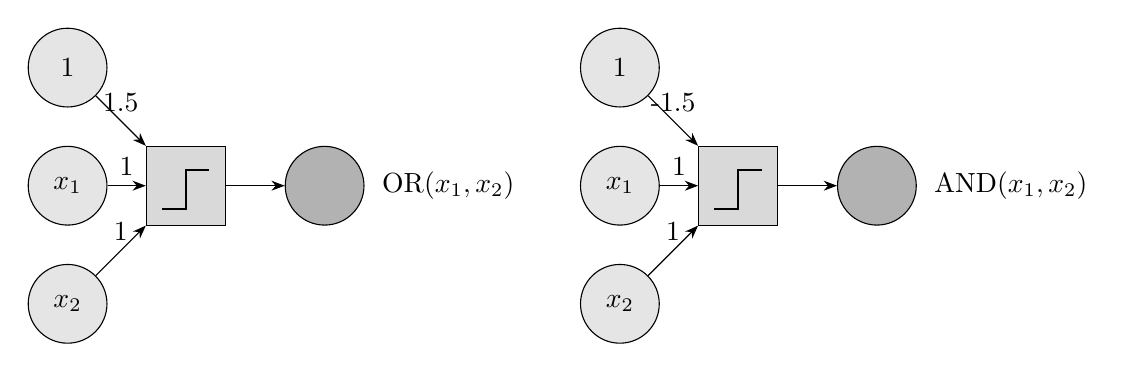
\begin{tikzpicture}[>=Stealth, node distance=1.5cm]

    % OR Perceptron
    \node[input neuron] (input1) {$1$};
    \node[input neuron, below of=input1] (inputx1) {$x_1$};
    \node[input neuron, below of=inputx1] (inputx2) {$x_2$};

    \node[activation function, right of=inputx1] (activation1) {};
    % Draw step function inside the activation node for OR
    % \draw (activation1.south west) -- (activation1.south west -| activation1.west) -- (activation1.north west -| activation1.east) -- (activation1.north east);

    \node[output neuron, right=0.75cm of activation1] (output1) {};
    \draw[->] (activation1) -- (output1);

    \node[right=0.1cm of output1] (or) {OR$(x_1, x_2)$};

    \draw[->] (input1) -- (activation1) node[midway,above] {1.5};
    \draw[->] (inputx1) -- (activation1) node[midway,above] {1};
    \draw[->] (inputx2) -- (activation1) node[midway,above] {1};

    % AND Perceptron
    \node[input neuron, right=6cm of input1] (input3) {$1$};
    \node[input neuron, below of=input3] (inputx3) {$x_1$};
    \node[input neuron, below of=inputx3] (inputx4) {$x_2$};

    \node[activation function, right of=inputx3] (activation2) {};
    % Draw step function inside the activation node for AND
    % \draw (activation2.south west) -- (activation2.south west -| activation2.west) -- (activation2.north west -| activation2.east) -- (activation2.north east);

    \node[output neuron, right=0.75cm of activation2] (output2) {};
    \draw[->] (activation2) -- (output2);

    \node[right=0.1cm of output2] (and) {AND$(x_1, x_2)$};

    \draw[->] (input3) -- (activation2) node[midway,above] {-1.5};
    \draw[->] (inputx3) -- (activation2) node[midway,above] {1};
    \draw[->] (inputx4) -- (activation2) node[midway,above] {1};

\end{tikzpicture}
    \caption{Implementing AND and OR gates with perceptrons}
    \label{fig:multi-percep2}
\end{figure}


\subsection{How a neural network operates}
\begin{figure}[H]
    \centering
    \includegraphics[width=0.5\linewidth]{img/nn.png}
    
    
\end{figure}

We can formally define neural networks based on their weights $w_{ij}^{(l)}$ and outputs $x^{(l)}_j$ which are just outputs of the activation function $\theta$ given their input from the previous layer, multiplied by the current layer's weights.\\

Input \textbf{x} is applied to the input layer $x_{1}^{(0)},\ldots,x_{d^{(0)}}^{(0)}\quad$ giving us $\quad x_{1}^{(L)}=h(\mathbf{x}).$

Note that we have $d$ dimensions
\[\begin{aligned}w_{ij}^{(l)}&\quad\begin{cases}1\le l\le L&\text{layers}\\0\le i\le d^{(l-1)}&\text{inputs}\\1\le j\le d^{(l)}&\text{outputs}\end{cases}\\\\\\x_j^{(l)}&=\theta(s_j^{(l)})=\theta\left(\sum_{i=0}^{d^{(l-1)}}w_{ij}^{(l)}x_i^{(l-1)}\right)\end{aligned}\]


There are different kinds of activation functions $\theta$ we can use:

\begin{itemize}
    \item Sigmoid Function: \(\theta(s) = \frac{1}{1 + e^{-s}}\)
    \item Hyperbolic Tangent Function: \(\tanh(s) = \frac{e^{s} - e^{-s}}{e^{s} + e^{-s}} = 2\sigma(2s) - 1\)
    \item Rectified Linear Unit (ReLU): \(\theta(s) = \max(0, s)\)
    \item Leaky Rectified Linear Unit (Leaky ReLU): \(\theta(s) = \max(\alpha s, s)\)
    \item Maxout: \(\theta(s) = \max(\alpha_1 s + \beta_1, \alpha_2 s + \beta_2)\)
    \item Exponential Linear Unit (ELU): \(\theta(s) = \max(\alpha(e^{s} - 1), s)\)
\end{itemize}

\begin{figure}[H]
    \centering
    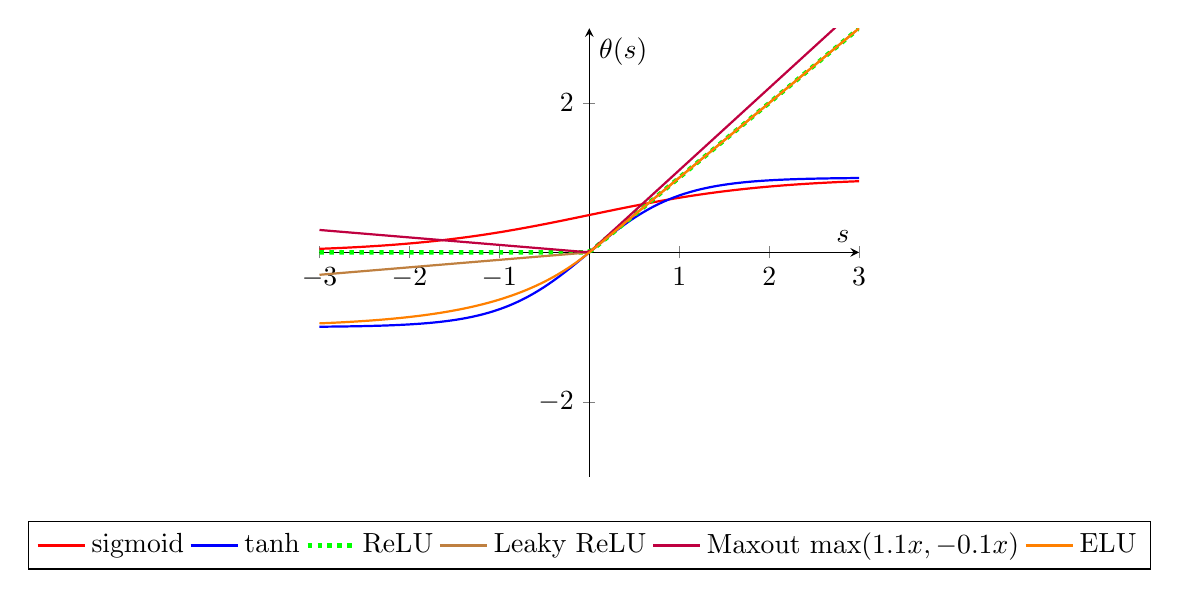
\begin{tikzpicture}
    \begin{axis}[
    axis lines=middle,
    xmin=-3, xmax=3,
    ymin=-3, ymax=3,
    xlabel={$s$},
    ylabel={$\theta(s)$},
    legend style={at={(0.5,-0.1)},anchor=north,legend columns=-1},
    cycle list name=color list
]

    % Sigmoid function
    \addplot[domain=-3:3, samples=100, red, thick] {1/(1 + exp(-x))};
    \addlegendentry{sigmoid}

    % Tanh function
    \addplot[domain=-3:3, samples=100, blue, thick] {tanh(x)};
    \addlegendentry{tanh}

    % ReLU function
    \addplot[domain=-3:3, samples=100, green, ultra thick, dotted] {max(0, x)};
    \addlegendentry{ReLU}
    % Leaky ReLU function
    \addplot[domain=-3:3, samples=100, brown, thick] {(x < 0) * 0.1 * x + (x >= 0) * x};
    \addlegendentry{Leaky ReLU}

    % Maxout function (example with alpha_1=1, beta_1=1, alpha_2=-1, beta_2=0)
    \addplot[domain=-3:3, samples=100, purple, thick] {max(1.1*x, -0.1*x)};
    \addlegendentry{Maxout $\max(1.1x, -0.1x)$}

    % ELU function
    \addplot[domain=-3:3, samples=100, orange, thick] {(x < 0) * (exp(x) - 1) + (x >= 0) * x};
    \addlegendentry{ELU}

    \end{axis}
    \end{tikzpicture}
    \caption{Common Activation Functions}
    \label{fig:actv-funcs}
\end{figure}

% \[
% \theta(s) = \tanh(s) = \frac{e^s - e^{-s}}{e^s + e^{-s}}
% \]

% \begin{figure}[H]
%     \centering
% \begin{tikzpicture}
% \begin{axis}[
%     axis lines=middle,
%     xmin=-3, xmax=3,
%     ymin=-1.5, ymax=1.5,
%     xlabel={$s$},
%     ylabel={$\theta(s)$},
%     legend pos=north west
% ]

% % Linear function
% \addplot[domain=-3:3, samples=2, green, thick] {x};
% \addlegendentry{linear}

% % Tanh function
% \addplot[domain=-3:3, samples=100, blue, thick] {tanh(x)};
% \addlegendentry{tanh}

% % Hard threshold (step) function
% \addplot[domain=-3:0, samples=2, red, thick] {-1};
% \addplot[domain=0:3, samples=2, red, thick] {1};
% \addlegendentry{hard threshold}

% \end{axis}
% \end{tikzpicture}
%     \caption{Activation Functions}
%     \label{fig:actv-funcs}
% \end{figure}


\subsection{Backward Computation}
\begin{figure}[H]
    \centering
    \includegraphics[width=1\linewidth]{img/nnbc.png}
    
    
\end{figure}
\subsection{Backpropagation Algorithm}\label{BackPropAlgo}
Backpropagation is a cornerstone algorithm for training neural networks. It efficiently computes the gradient of the loss function with respect to the weights of the network.


\begin{definitionbox}{Backpropagation Algorithm Steps}
\begin{enumerate}
    \item Initialize all network weights \( w_{ij}^{(l)} \) randomly to break symmetry.
    \item For each iteration \( t = 1, 2, \ldots \) until convergence:
    \begin{enumerate}
        \item Select a data point \( (x_k, y_k) \) randomly or sequentially.
        \item \textbf{Forward Pass}:
        \begin{itemize}
            \item Compute the activation \( x_j^{(l)} \) of each layer \( l \) starting from the input layer and progressing through to the output layer.
        \end{itemize}
        \item \textbf{Backward Pass}:
        \begin{itemize}
            \item Compute the gradient of the loss function with respect to the activations \( \delta_j^{(l)} \), starting from the output layer and propagating back to the input layer.
        \end{itemize}
        \item \textbf{Update Weights}:
        \begin{itemize}
            \item Adjust the weights \( w_{ij}^{(l)} \) in the direction that most reduces the loss, typically using a learning rate \( \eta \) and the gradient \( \delta_j^{(l)} \).
            \item The update can be done using a single data point (Stochastic Gradient Descent), a minibatch of data points, or the entire dataset (batch gradient descent).
        \end{itemize}
    \end{enumerate}
    \item After sufficient iterations or upon convergence, return the final weights \( w_{ij}^{(l)} \).
\end{enumerate}
\end{definitionbox}

\subsection*{Regularisation Techniques}
Regularisation is employed to prevent overfitting and improve generalisation. Common techniques include:
\begin{itemize}
    \item \( L2 \) regularisation (weight decay): Adds a penalty term to the loss function proportional to the sum of the squares of the weights.
    \item \( L1 \) regularisation: Adds a penalty proportional to the sum of the absolute values of the weights.
    \item Dropout: During training, randomly sets a subset of weights to zero to prevent co-adaptation of neurons.
\end{itemize}

\begin{examplebox}{Example Neural Networks Question}
\begin{figure}[H]
    \centering
    \includegraphics[width=0.5\linewidth]{img/nn_eg_q.png}
\end{figure}

\subsubsection*{Question}
Given this neural network, propose a non-linearity activation function, draw this function and its gradient in a figure.

\subsubsection*{Solution:}
% \begin{figure}[H]
%     \centering
%     \includegraphics[width=0.5\linewidth]{img/eg_sol_nn.png}
    
    
% \end{figure}


\begin{figure}[H]
    \centering
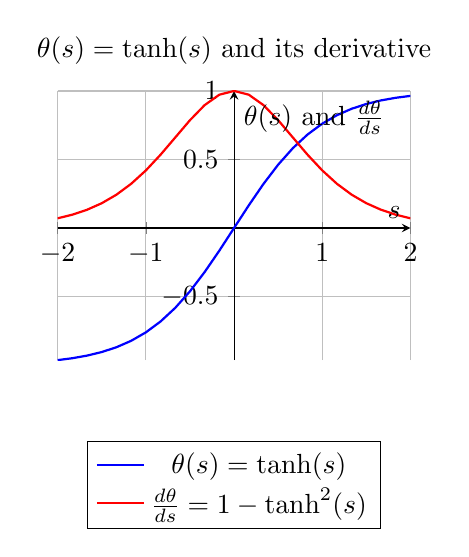
\begin{tikzpicture}
\begin{axis}[
    title={$\theta(s) = \tanh(s)$ and its derivative},
    axis lines=middle,
    width=0.5\textwidth,
    height=5cm,
    grid=major,
    domain=-2:2,
    legend style={at={(0.5,-0.3)},anchor=north },
    xlabel={$s$},
    ylabel={$\theta(s)$ and $\frac{d\theta}{ds}$},
]
% tanh function
\addplot[blue, thick] {tanh(x)};
\addlegendentry{$\theta(s) = \tanh(s)$}

% derivative of tanh function
\addplot[red, thick] {1 - (tanh(x))^2};
\addlegendentry{$\frac{d\theta}{ds} = 1 - \tanh^2(s)$}
\end{axis}
\end{tikzpicture}
\\

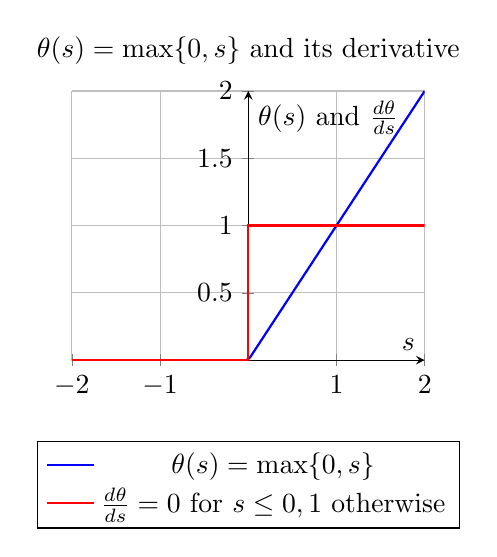
\begin{tikzpicture}
\begin{axis}[
    title={$\theta(s) = \max\{0, s\}$ and its derivative},
    axis lines=middle,
    width=0.5\textwidth,
    height=5cm,
    grid=major,
    domain=-2:2,
    legend style={at={(0.5,-0.3)},anchor=north },
    xlabel={$s$},
    ylabel={$\theta(s)$ and $\frac{d\theta}{ds}$},
    samples=100,
]
% ReLU function
\addplot[blue, thick] {max(0,x)};
\addlegendentry{$\theta(s) = \max\{0, s\}$}

% derivative of ReLU function
\addplot[red, thick, const plot mark mid] {x > 0 ? 1 : 0};
\addlegendentry{$\frac{d\theta}{ds} = 0 \text{ for } s \leq 0, 1 \text{ otherwise}$}

\end{axis}
\end{tikzpicture}
\end{figure}


\subsubsection*{Question}
Discuss what happens if we use \( x \) as input, \( \theta(s) = s \) as the activation function and \( W_l \) as a matrix of weights in layer \( l \). Can \( \theta(s) = s \) be achieved with \( \text{tanh}(s) \)?

\subsubsection*{Solution:} 
If the activation function is the identity function \( \theta(s) = s \), then the output of each layer in the neural network is a linear transformation of the input. The network effectively becomes a single linear model, as all weights between layers can be directly multiplied, like a product of matrices $\mathbf{w}_{L}^{\top}W_{L-1}W_{L-2}\ldots W_{1}\mathbf{x}=\mathbf{w}_{*}^{\top}\mathbf{x}$. This is because because the composition of linear functions is itself a linear function.\\

This means that the overall network can only represent linear relationships between the input and output.\\

\( \text{tanh}(s) \) is a non-linear function, and their general use is what allows neural networks to capture non-linearities and complex patterns in the data.\\

Therefore in general, \( \theta(s) = s \) cannot be achieved with \( \text{tanh}(s) \) because \( \text{tanh}(s) \) is non-linear. However, \(\text{tanh}(s) \) does approximate the linear function partially, so using regularisation, we can shrink the weights and biases so the output of \( \text{tanh}(s) \) is approximately linear for the range of inputs the network receives, then \( \text{tanh}(s) \) could approximate \( \theta(s) = s \).

\begin{figure}[H]
\centering
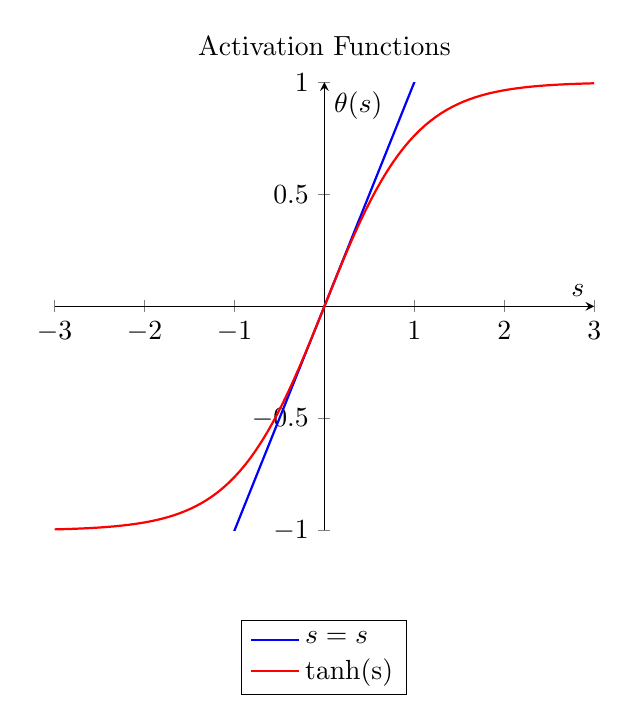
\begin{tikzpicture}
\begin{axis}[
    axis lines=middle,
    xmin=-3, xmax=3,
    ymin=-1, ymax=1,
    xlabel={$s$},
    ylabel={$\theta(s)$},
    legend style={at={(0.5,-0.2)},anchor=north},
    legend cell align={left},
    cycle list name=color list,
    title={Activation Functions}
]
% Linear function
\addplot[domain=-3:3, samples=100, blue, thick] {x};
\addlegendentry{$s=s$}

% Tanh function
\addplot[domain=-3:3, samples=100, red, thick] {tanh(x)};
\addlegendentry{tanh(s)}

\end{axis}
\end{tikzpicture}
\caption{Linear and Hyperbolic Tangent Activation Functions}
\end{figure}


\subsubsection*{Question}
Given input vector \( \mathbf{x} = (4, -8, 4) \) use the proposed non-linearity from question i) to calculate outputs of all neurons and \( h(\mathbf{x}) \).

\subsubsection*{Solution:}
The outputs \( x_j^{(l)} \) are calculated by applying the activation function \( \theta(s) \) to the weighted sum of the inputs:
\[ x_j^{(l)} = \theta\left( \sum_{i=0}^{d^{(l-1)}} w_{ij}^{(l)} x_i^{(l-1)} \right). \]
Using the ReLU activation function \( \theta(s) = \max(0, s) \), we get:
\begin{align*}
f_a &= \max(0, 1 + 0.25 \cdot 4 + 0.75 \cdot (-8) + 0.75 \cdot 4) = 0, \\
f_b &= \max(0, 1 + 0.5 \cdot 4 + 0.125 \cdot (-8) + 0.25 \cdot 4) = 3, \\
h(\mathbf{x}) &= f_c = \max(0, 0.5 + 0.5 \cdot 0 + 0.125 \cdot 3) = 0.875.
\end{align*}



\subsubsection*{Question}
Given the learning rate \( \eta = 0.1 \), ReLU activation, and a training example \( x = (4, -8, 4) \) with its label \( y = 2 \), we want to apply the backpropagation algorithm to update the weight \( w_{3,b}^{(2)} \) using the \( L_2 \) loss function without regularisation.

\subsection*{Solution:}
Using the outputs from forward propagation, the \( L_2 \) loss function \( \ell_2(f_c, y) \) is given by:
\[ \ell_2(f_c, y) = \frac{1}{2}(f_c - y)^2 = \frac{1}{2}(0.875 - 2)^2 = 0.63. \]

Since we are using ReLU activation, the derivative of the activation function \( \theta'(s) \) with respect to the pre-activation \( s \) is:
\[ \theta'(s) = \frac{\partial}{\partial c} \max(0, c) = 
\begin{cases} 
1 & \text{if } c > 0 \\
0 & \text{otherwise}
\end{cases}.
\]

The gradient of the loss with respect to the output of neuron \( c \) is:
\[ \frac{\partial \ell}{\partial f_c} = (f_c - y) = (0.875 - 2) = -1.125. \]

The error term \( \delta_c \) for neuron \( c \) is the same as the gradient since the derivative of ReLU for positive inputs is 1:
\[ \delta_c = \frac{\partial \ell}{\partial f_c} \frac{\partial f_c}{\partial c} =\frac{\partial \ell}{\partial f_c}  \frac{\partial  \max(0, c) }{\partial c}= -1.125. \]

The gradient of the loss with respect to the weight \( w_{3,b}^{(2)} \) is:
\[ \delta_b = \delta_c \frac{\partial c}{\partial w_{3,b}^{(2)}} = -1.125 \cdot 0.125 = -0.14. \]

The weight update rule for \( w_{3,b}^{(2)} \) is:
\[ w_{3,b}^{(2)} \leftarrow w_{3,b}^{(2)} - \eta x_3 \delta_b. \]

Substituting the values, we get:
\[ w_{3,b}^{(2)} \leftarrow w_{3,b}^{(2)} + 0.1 \cdot 4 \cdot 0.14. \]

\subsubsection*{Question}
Write down the main steps of the backpropagation algorithm.

\subsubsection*{Solution:} See \ref{BackPropAlgo}

\subsubsection*{Question}
What is the role of the learning rate in gradient descent and what are the risks of setting the learning rate too large or too small?

\subsubsection*{Solution:}
The learning rate \( \eta \) affects the speed of convergence. A small \( \eta \) may result in a very long optimisation process, whereas a large \( \eta \) can lead to oscillations near the function's minimum or cause divergence.

\end{examplebox}
\subsection{Remarks on Neural Networks}

\begin{itemize}
    \item Any kind of features can be learned, Neural Networks are called universal approximators as a result. Also, adding extra hidden layers may exponentially reduce the number of nodes needed.
    \item They are hard to interpret, and may not generalise well as their VC-dimensions are usually high.
    \item They achieve state-of-the-art performance in many areas, in different forms, such as Convolutional Neural Networks (CNN) for image processing and Recurrent Neural Networks (RNN) for speech and natural language processing.
    \item They work well with a lot of data, and can be used with various regularisers and target functions.
\end{itemize}

% All the weights $\mathbf{w} = \{w_{ij}^{(l)}\}$ determine $h(\mathbf{x})$

% Error on example $(\mathbf{x}_n, y_n)$ is

% \[ e(h(\mathbf{x}_n), y_n) = e(\mathbf{w}) \]

% To implement SGD, we need the gradient

% \[ \nabla e(\mathbf{w}): \frac{\partial e(\mathbf{w})}{\partial w_{ij}^{(l)}} \text{ for all } i, j, l \]

\chapter{Geometric Classification}
\begin{commentbox}{IMPORTANT!}
    Before finidng support vectors, you must scale all attributes to have zero mean and unit variance, in order to match the canonical hyperplane. 
\end{commentbox}
\section{Support Vector Machines}
\begin{figure}[H]
    \centering
    \includegraphics[width=0.75\linewidth]{img/svg_max_margin.png}
    \caption{Intuitively, in classification, a larger margin is better}
    \label{fig:svm_max_margin-label}
\end{figure}
\begin{figure}[H]
    \centering
    \includegraphics[width=0.5\linewidth]{img/middlestreet.png}
    \caption{For any $u$ during testing, our prediction is $sign(w\top u+ b)$}
    \label{fig:middlestreet-label}
\end{figure}

\subsection{Maximising the Margin}
\label{subsec:maximising_margin}

Intuitively, in classification tasks, a large margin between the classes is desirable as it may lead to better generalization from the training data to unseen data. This concept is often referred to as the ``widest street'' approach, where the margin is analogous to the width of the street. The goal of the SVM algorithm is to find the hyperplane that ``paves'' this widest street between the data points of different classes, hence maximising the margin.

\subsubsection*{Distance to a Hyperplane}
The distance from a point \( \mathbf{x} \) to a hyperplane defined by \( \mathbf{w}^T \mathbf{x} + b = 0 \) can be given by the formula:
\[
\text{Distance} = \frac{|\mathbf{w}^T \mathbf{x} + b|}{\|\mathbf{w}\|}.
\]
Here, the vector \( \mathbf{p}_{\mathbf{x}} \) represents the orthogonal projection of \( \mathbf{x} \) onto the hyperplane:
\[
\mathbf{p}_{\mathbf{x}} = \mathbf{x} - \frac{(\mathbf{w}^T \mathbf{x} + b)}{\|\mathbf{w}\|^2}\mathbf{w}.
\]
The vector \( \mathbf{x} - \mathbf{p}_{\mathbf{x}} \) is parallel to \( \mathbf{w} \) and thus orthogonal to the hyperplane, which confirms that \( \mathbf{p}_{\mathbf{x}} \) is indeed the orthogonal projection. Moreover, any vector \( \mathbf{u} \) in the hyperplane satisfies \( \mathbf{w}^T \mathbf{u} = 0 \) (orthogonal to \( \mathbf{w} \)), which underpins the definition of the orthogonal projection. The relationship between the norm of \( \mathbf{x} \) and its projection is:
\[
\|\mathbf{x}\|^2 = \|\mathbf{x} - \mathbf{p}_{\mathbf{x}} + \mathbf{p}_{\mathbf{x}}\|^2 = \|\mathbf{x} - \mathbf{p}_{\mathbf{x}}\|^2 + \|\mathbf{p}_{\mathbf{x}}\|^2,
\]
holding true by the Pythagorean theorem as \( \mathbf{x} - \mathbf{p}_{\mathbf{x}} \) and \( \mathbf{p}_{\mathbf{x}} \) are orthogonal.

\subsubsection*{Hard-Margin SVM}
In the context of SVMs, the points are separable if there exist weights \( \mathbf{w} \) and bias \( b \) such that \( y_i(\mathbf{w}^T \mathbf{x}_i + b) > 0 \) for each data point \( \mathbf{x}_i \) with label \( y_i \in \{-1, +1\} \). The margin of the SVM classifier is the minimum distance from any point to the hyperplane \( H(\mathbf{w}, b) \), defined as:
\[
\delta^* \equiv \min_i \frac{|\mathbf{w}^T \mathbf{x}_i + b|}{\|\mathbf{w}\|} = \min_i y_i\left(\frac{\mathbf{w}^T \mathbf{x}_i + b}{\|\mathbf{w}\|}\right).
\]
The points that lie exactly at distance \( \delta^* \) from the hyperplane are called support vectors. Therefore, a point \( \mathbf{x}^* \) is a support vector if and only if:
\[
\frac{|\mathbf{w}^T \mathbf{x}^* + b|}{\|\mathbf{w}\|} = \delta^*.
\]
The optimisation problem in SVMs is thus to maximise \( \delta^* \), the margin, by adjusting \( \mathbf{w} \) and \( b \), which geometrically corresponds to finding the widest possible street between the classes.

\begin{figure}[H]
    \centering
    \includegraphics[width=0.5\linewidth]{img/convexhull.png}
    \caption{The two closest points of the convex hulls (the smallest convex set that contains all the points) determine the separating plane.}
    
\end{figure}
\subsection{Canonical Hyperplane}
There are many ways to describe a hyperplane, such that $H(w,b)$ and $H(\alpha w, \alpha b)$ will define the exact same set of points. 

To uniquely identify the separating hyperplane in SVM, we use the concept of a canonical hyperplane. A canonical hyperplane is defined such that for a given support vector \( \mathbf{x}^* \), the following condition holds:
\[
y^*(\mathbf{w}^T \mathbf{x}^* + b) = 1.
\]
This normalisation ensures that the distance from the support vector to the hyperplane is scaled such that it provides a consistent measure of confidence for predictions. The canonical form aids in the interpretation of SVM outputs, especially when comparing predictions for new data points.\\

Hence, for all support vectors, the above equation holds true, and for any other data point not on the margin boundary, the inequality \( y_i(\mathbf{w}^T \mathbf{x}_i + b) > 1 \) must be satisfied, as any point that is not the support vector must be farther away. This ensures that non-support vectors lie outside the margin defined by the support vectors. \\


For the remainder of the notes, it can be assumed that the margin for canonical hyperplanes is given by \( \delta^* = \frac{1}{\|\mathbf{w}\|} \), and it is this margin that we seek to maximise in SVM.\\

\subsubsection*{Maximum Margin Hyperplane}
The maximum margin hyperplane is the heart of the SVM classifier. The objective of SVM is to find the canonical hyperplane \( H(\mathbf{w}, b) \) which maximises the margin between the classes. The optimal hyperplane parameters \( (\mathbf{w}_*, b_*) \) are found by solving the following optimisation problem:
\[
(\mathbf{w}_*, b_*) = \arg\max_{\mathbf{w},b} \left\{ \frac{1}{\|\mathbf{w}\|} \right\} \text{ such that } y_i(\mathbf{w}^T \mathbf{x}_i + b) \geq 1, \forall i.
\]
This optimisation problem differs from the Perceptron algorithm, which continues to adjust its weights until all points are correctly classified, without necessarily maximizing the margin. The Perceptron stops as soon as it finds any solution that separates the data with zero error, without concern for the margin width or the generalisation of the classifier. In contrast, the SVM is designed to find the ``best'' solution by maximising the margin, leading to potentially better generalisation capabilities.

\subsection{Formulation of Hard-Margin SVM}
\label{subsec:formulation_hard_margin_svm}

The hard-margin SVM is formulated as an optimization problem where the goal is to minimize the norm of the weight vector \( \mathbf{w} \), which is directly related to maximizing the margin. The problem can be stated as:

\[
\text{minimize} \quad \frac{1}{2}\|\mathbf{w}\|^2
\]
\[
\text{subject to} \quad y_i(\mathbf{w}^T \mathbf{x}_i + b) \geq 1 \quad \text{for all} \quad i.
\]

The choice of \( \frac{1}{2} \) as a multiplier for the norm of \( \mathbf{w} \) is arbitrary and does not affect the solution; it is chosen for mathematical convenience as it simplifies the analysis, particularly when taking derivatives.\\

The choice of the squared Euclidean norm (Norm-2) over other norms (like the Manhattan norm, Norm-1) is not just for mathematical convenience.\\

Minimising the Euclidean Norm-2 tends to not penalise small values of \( \mathbf{w} \) as much, so they are not forced to approach zero, allowing all features to contribute.\\


Minimising the Manhattan Norm-1 treats all values equally, promoting sparsity in the solution, by penalising large and small values equally, akin to feature selection. \\

Usually in practice, minimising the squared Euclidean norm is less prone to overfitting compared to the Manhattan norm.

\subsubsection*{Lagrangian Formulation and the KKT Conditions}
The Lagrangian formulation introduces dual variables \( \alpha_i \) for each constraint in the optimisation problem, leading to the Lagrangian:
\[
L(\mathbf{w}, b, \boldsymbol{\alpha}) = \frac{1}{2}||\mathbf{w}||^2 + \sum_{i=1}^n \alpha_i[1 - y_i(\mathbf{w}^T \mathbf{x}_i + b)],
\]

where the goal is to minimise \( L \) with respect to \( \mathbf{w} \) and \( b \), and to maximise it with respect to the dual variables \( \alpha_i \geq 0 \).

The Karush-Kuhn-Tucker (KKT) conditions provide the necessary conditions for optimality in this context. They are given by:

\begin{align*}
\nabla_{\mathbf{w}}L &= \mathbf{w} - \sum_{i=1}^n \alpha_i y_i \mathbf{x}_i = 0  &\Rightarrow & \quad \mathbf{w} = \sum_{i=1}^n \alpha_i y_i \mathbf{x}_i, \\
\nabla_{b}L &= -\sum_{i=1}^n \alpha_i y_i = 0  &\Rightarrow & \quad \sum_{i=1}^n \alpha_i y_i = 0, \\
&\alpha_i[1 - y_i(\mathbf{w}^T \mathbf{x}_i + b)] = 0  &\Rightarrow & \quad \alpha_i = 0 \quad \text{or} \quad y_i(\mathbf{w}^T \mathbf{x}_i + b) = 1.
\end{align*}

Data points \( \mathbf{x}_i \) with corresponding \( \alpha_i \neq 0 \) are known as support vectors. These are the points that lie on the margin, and hence, \( y_i(\mathbf{w}^T \mathbf{x}_i + b) = 1 \) for support vectors. Importantly, the weight vector \( \mathbf{w} \) is expressed as a linear combination of the support vectors, showing the role they play in defining the decision boundary.

\begin{commentbox}{KKT Conditions}
The KKT conditions for optimality are a set of necessary conditions for a solution to be optimal in a mathematical optimisation problem. They are necessary and sufficient conditions for a local minimum in nonlinear programming problems.
\end{commentbox}

\begin{definitionbox}{Hard-SVM Dual Formulation}
    We can fine the dual-formulation for the Hard-SVM problem as follows:
    \[
    \max_\alpha\mathcal{L}(\alpha)\triangleq\sum_{i=1}^n\alpha_i-\frac12\sum_{i=1}^n\sum_{j=1}^ny_iy_j\alpha_i\alpha_jx_i^\top x_j
    \]

    subject to \[\alpha_{i}\geq0,\sum_{i=1}^{n}\alpha_{i}y_{i}=0.\]
    
\end{definitionbox}
In the context of SVMs, after solving for the Lagrange multipliers $\alpha_i^*$, the weight vector $\mathbf{w}^*$ and the bias term $b^*$ can be computed as follows:\\

The optimal weight vector is determined by the sum over all support vectors, denoted by non-zero $\alpha_i^*$, and is given by:
\[
\mathbf{w}^* = \sum_{i:\alpha_i^*>0} \alpha_i^* y_i \mathbf{x}_i
\]

The optimal bias term $b^*$ ensures that the decision boundary correctly classifies the support vectors. For any support vector $\mathbf{x}_i$, the following condition holds:
\[
y_i( (\mathbf{w}^*)^\top \mathbf{x}_i \rangle + b^*) = 1
\]
This can be rearranged to solve for $b^*$ using any support vector $\mathbf{x}_i$:
\[
b^* = \frac{1}{y_i} -  (\mathbf{w}^*)^\top\mathbf{x}_i = y_i - (\mathbf{w}^*)^\top\mathbf{x}_i
\]
Since all support vectors lie on the margin, and their $\alpha_i^*$ are non-zero, this formula will give the same result irrespective of the chosen support vector $\mathbf{x}_i$.\\

The above conditions provide a way to construct the separating hyperplane that maximises the margin between the two classes in the feature space, which is the essence of the hard-margin SVM.


\subsubsection*{Prediction with Hard-SVM}
Assume we fit our model to a training dataset, and want to make a new prediction for new data sample $x$. We predict $\hat{y} = 1$ if and only if $(w^*(^\top x + b^* >0$\\

We have
\begin{align*}
(w^{*})^{T}x+b^{*}& =\left(\sum_{i=1}\alpha_i^*y_ix_i\right)^{\prime}x+b^*  \\
&=\sum_{i=1:\alpha_i^*>0}^n\alpha_i^*y_i(x_i^Tx)+b^*
\end{align*}


\subsection{Soft-Margin SVM}

Sometimes, when data is non-linearly separable, we cannot guarantee points will be classified correctly such that $y_i(w^\top x_i+b)\geq1\text{ for all i}$. \\


In the soft-margin SVM, the introduction of slack variables \( \xi_i \) relaxes this condition, and allows some misclassifications. The optimisation problem can be written as:

\[
\min_{\mathbf{w},b,\boldsymbol{\xi}} \quad \frac{1}{2} \lVert \mathbf{w} \rVert^2 + C \sum_{i=1}^n \xi_i
\]

\[
\text{subject to} \quad y_i(\mathbf{w}^\top \mathbf{x}_i + b) \geq 1 - \xi_i \quad \text{and} \quad \xi_i \geq 0 \quad \forall i
\]

The parameter \( C \) in the soft-margin SVM controls the trade-off between maximising the margin and minimising the classification error. It enforces an upper bound on the norm of the weights.\\

A large C penalises even small margin violations, and a small C means we can freely violate the margin for some points as long as it helps make the margin wider. It provides a balance between minimising $||\textbf{w}||^2$\\ keeping a large margin, and minimising misclassified samples.\\

The Lagrangian of the soft-margin SVM is given by the hard-margin objective plus three additional terms incorporating the slack variables:

\[
\mathcal{L}(\mathbf{w}, b, \boldsymbol{\alpha}, \boldsymbol{\beta}) = \frac{1}{2} \lVert \mathbf{w} \rVert^2 +  \underbrace{C\sum_{i=1}^n \xi_i}_{\text{ soft margin }} - \sum_{i=1}^n \alpha_i [y_i(\mathbf{w}^\top \mathbf{x}_i + b) - 1 + \underbrace{\xi_i}_\text{ soft margin }] - \underbrace{\sum_{i=1}^n \beta_i \xi_i}_{\text{ soft margin }}
\]

To minimise in primal variables \( \mathbf{w}, b, \boldsymbol{\xi} \), and maximise in dual variables \( \boldsymbol{\alpha}, \boldsymbol{\beta} \geq 0 \), we apply the Karush-Kuhn-Tucker (KKT) conditions:

\begin{align*}
\nabla_{\mathbf{w}} \mathcal{L} &=  \mathbf{w} = \sum_{i=1}^n \alpha_i y_i \mathbf{x}_i = 0 \quad &\Rightarrow& \quad \mathbf{w} = \sum_{i=1}^n \alpha_i y_i \mathbf{x}_i\\
\nabla_b \mathcal{L} &= -\sum_{i=1}^n \alpha_i y_i = 0 \quad &\Rightarrow& \quad \sum_{i=1}^n \alpha_i y_i = 0\\
\nabla_{\xi_i} \mathcal{L} &= C - \alpha_i - \beta_i = 0 \quad &\Rightarrow& \quad C = \alpha_i + \beta_i\\
&\alpha_i (1 - \xi_i - y_i(\mathbf{w}^\top \mathbf{x}_i + b)) = 0 &\Rightarrow& \quad \alpha_i = 0\text{ or } y_i(\textbf{w}^\top x_i + b) = 1-\xi_i\\
&\beta_i \xi_i = 0 &\Rightarrow& \quad \beta_i = 0 \text{ or } \xi_i = 0
\end{align*}





The last two conditions above are known as the complementary slackness conditions. They imply that for any \( i \), either \( \alpha_i = 0 \) or \( y_i(\mathbf{w}^\top \mathbf{x}_i + b) = 1 - \xi_i \). Also, if \( \alpha_i = C \), then the corresponding point \( (\mathbf{x}_i, y_i) \) lies on or within the margin, or it is misclassified.\\

The introduction of the slack variable \( \xi_i \) in the soft-margin SVM leads to an additional constraint in the dual optimisation problem, which restricts the Lagrange multipliers for each data point:

\[
0 \leq \alpha_i \leq C
\]

This constraint ensures that the dual variables \( \alpha_i \) are bounded above by \( C \), reflecting the trade-off between margin width and classification error.

\begin{figure}[H]
    \centering
\includegraphics[width=0.5\linewidth]{img/large-small-margin.png}
    \caption{Comparing different effects of C sizes}
    
    \includegraphics[width=0.8\linewidth]{img/svm_C.png}
    \caption{C is essentially a regularisation parameter, which controls the trade-off between: achieving a low error on the training data (larger C) and minimising the norm of the weights (smaller C). The most common method for finding appropriate C is cross validation.}
    
\end{figure}

Note that a soft-margin helps with in-training accuracy on data that can generally be linearly separable, but it alone cannot improve performance on data that that requires major feature space transformations.

\subsection{Soft-margin SVM Dual}

The dual formulation of the soft-margin SVM focuses on optimising the Lagrange multipliers \(\alpha_i\). The dual objective function to be minimised is:

\[
\mathcal{L}(\alpha) = \sum_{i=1}^{n} \alpha_i - \frac{1}{2} \sum_{i=1}^{n} \sum_{j=1}^{n} y_i y_j \alpha_i \alpha_j  \mathbf{x}_i^\top \mathbf{x}_j 
\]

This is subject to the constraints:

\[
0 \leq \alpha_i \leq C, \quad \text{and} \quad \sum_{i=1}^{n} \alpha_i y_i = 0
\]

From the dual variables, we can compute the weight vector \(\mathbf{w}^*\) as follows:

\[
\mathbf{w}^* = \sum_{i:\alpha_i^*>0} \alpha_i^* y_i \mathbf{x}_i
\]

The bias term \(b^*\) can be solved by using any support vector \(\mathbf{x}_i\) that lies on the margin, which is characterised by \(0 < \alpha_i < C\) and \(\xi_i = 0\). It is computed as:

\[
b^* = \frac{1}{y_i} - (\mathbf{w}^*)^\top \mathbf{x}_i = y_i - (\mathbf{w}^*)\top x_i
\]


Finally, classification of new samples can be performed using the sign of the decision function:

\[
\hat{y} = \text{sign}((\mathbf{w}^*)^\top \mathbf{x} + b^*)
\]

This formulation allows us to predict the class label of a new sample \(\mathbf{x}\) by considering the sign of the linear combination of the support vectors, weighted by the corresponding \(\alpha_i^*\), and adjusted by the bias term \(b^*\).


\subsection{Non-Linear Transformations and Kernels}

\subsubsection*{Intro to Kernels}
Kernel functions are a way of computing the dot product of two vectors $x$ and $y$ in some feature space, that could be possibly be very high dimensional. They are also called the `generalised dot product'. Intuitively, they are a similarity function that outputs a similarity score given two objects.

\begin{figure}[H]
    \centering
\includegraphics[width=0.5\linewidth]{img/kernel.png}
    
    
\end{figure}


In SVMs with non-linear transformations, the input data \( x \) is transformed into a higher dimensional space using a function \( \phi \). This enables the linear separation of data that is not linearly separable in the original input space. The transformed feature space is represented by \( z = \phi(x) \).\\

\subsubsection*{Lagrangian in Dual Form}

The dual formulation of the SVM with these transformations becomes (swapping $x_i$ with transformed $z_i$):

\[
\mathcal{L}(\alpha) = \sum_{i=1}^n \alpha_i - \frac{1}{2} \sum_{i=1}^n \sum_{j=1}^n y_i y_j \alpha_i \alpha_j z_i^\top z_j
\]

subject to:

\[
0 \leq \alpha_i \leq C, \quad \sum_{i=1}^n \alpha_i y_i = 0.
\]

\subsubsection*{Classification in SVM}

To classify new samples, we use the decision function:

\[
g(x) = \text{sign}(w^\top z + b)  = \text{sign} \left( \sum_{i:\alpha_i>0, z_i \text{is support vector}} \alpha_i y_i z_i^\top z + b \right),
\]

where \( b \) is calculated from any support vector \( z_i \):

\[
b = 1 - y_i w^\top z_i.
\]


So to solve this problem all we need is the transformed data in the form $z_i^\top z_j$.\\

\subsubsection*{The Kernel Function}

The kernel function is defined as the dot product of two distinct transformed vectors of $\textbf{x}$:
\begin{equation*}
    K(\mathbf{x}, \mathbf{x'}) = \langle \phi(\mathbf{x}), \phi(\mathbf{x'}) \rangle = \mathbf{z}^\top \mathbf{z}'
\end{equation*}
where $\phi$ is a transformation that maps the input data to a higher-dimensional space, and $\langle \cdot, \cdot \rangle$ denotes the inner product.

\subsubsection*{Polynomial Kernel Function Example}
Consider a two-dimensional input vector $\mathbf{x} = (x_1, x_2)$. We also have a polynomial transform of degree 2:
\begin{align*}
    \mathbf{z} &= \phi(\mathbf{x}) = (1, x_1, x_2, x_1^2, x_2^2) \\
\end{align*}
The polynomial kernel of degree 2 is given by:
\begin{align*}
    K(\mathbf{x}, \mathbf{x'}) = \mathbf{z}^\top \mathbf{z} &= 1 + x_1x_1' + x_2x_2' + x_1^2{x_1'}^2 + x_2^2{x_2'}^2
\end{align*}


We can also derive kernels straightaway and work out $\textbf{z}$ later:
\begin{align*}  K(\mathbf{x},\mathbf{x}^{\prime})& =(1+\mathbf{x}^\top\mathbf{x}^\prime)^2=(1+x_1x_1^\prime+x_2x_2^\prime)^2  \\
&=1+x_1^2{x_1^{\prime}}^2+x_2^2{x_2^{\prime}}^2+2x_1x_1^{\prime}+2x_2x_2^{\prime}+2x_1x_2x_1^{\prime}x_2^{\prime}
\end{align*}

The inner product for $\textbf{z}$ is:
\begin{equation*}
    \mathbf{z} = (1, x_1^2, x_2^2, \sqrt{2}x_1, \sqrt{2}x_2, \sqrt{2}x_1x_2)
\end{equation*}




\subsubsection*{Linear Kernel Example}
The linear kernel is simply the dot product in the input space, representing the similarity of $\mathbf{x}$ and $\mathbf{x'}$:
\begin{equation*}
    K(\mathbf{x}, \mathbf{x'}) = \mathbf{x}^\top \mathbf{x'}
\end{equation*}


\subsubsection*{Properties of Kernel Functions}

\begin{itemize}
    \item Kernels provide a compact representation of the data in the transformed feature space.
    \item The choice of kernel is task-specific and greatly influences the performance of the SVM.
    \item The best way to determine the appropriate kernel and its parameters is through cross-validation.
\end{itemize}

The kernel function \( K(x, x') \) replaces the dot product in the feature space, allowing us to compute the similarity between two points in the original input space without explicitly computing their coordinates in the feature space. \\


Kernels can be understood as a compact representation of the classification task's knowledge, encapsulating the structure of the data in the transformation \( \phi \) that they implicitly apply. The choice of kernel is task-specific and often determined through cross-validation to achieve the best classification performance.\\

Non-linear kernels like the polynomial kernel allow more complex relationships by considering not just the direct similarity but also the interactions between the features of \( \textbf{x} \) and \( \textbf{x'} \).

\subsubsection*{Gaussian (Radial Basis Function -  RBF) Kernel}

Consider this feature map in $\mathbb{R}$:

\[
\phi(x)_n=\frac1{\sqrt{n!}}\exp-x^2/2x^n
\]

\[
\begin{aligned}
\phi(x)^T\phi(x^{\prime})& =\sum_{n=0}^\infty\left(\frac1{\sqrt{n!}}e^{-x^2/2}x^n\right)\left(\frac1{\sqrt{n!}}\mathrm{e}^{-(x^{\prime})^2/2}(x^{\prime})^n\right)  \\
&=e^{-\frac{x^2+(x^{\prime})^2}2}\sum_{n=0}^\infty\frac{(x\cdot x^{\prime})^n}{n!} \\
&=e^{-\frac{\|x-x^{\prime}\|^2}2}
\end{aligned}
\]

In this kernel, we take the squared distance between two datapoints instead of their dot product(s) as seen in the polynomial kernel. So the amount of influence one observation has on another is a function of the squared distance. \\

Intuitively we can see if the distance between them two datapoints are greater, the less influence they have on each other, because the kernel function evaluates to a smaller value (due to a negative sign in the power). This makes Gaussian RBF act a bit like a Nearest Neighbour classification.

We can further scale this influence by a factor $\gamma$ from cross validation:
\[K(x,x')=\exp\left(-\gamma\underbrace{\|x-x'\|^2}_{radial}\right)\]\\

\subsubsection*{SVM Predictor for Gaussian RBF}

THe SVM predictor for the Gaussian RBF can be written as:

\[g(x)=\text{sign}\left(\sum_{x_i\text{is SV}}\alpha_iy_iK(x_i,x)+b\right)=\text{sign}\left(\sum_{x_i\text{is SV}}\alpha_iy_ie^{-\gamma\|x-x_i\|^2}+b\right)\]

\begin{sidenotebox}{RBF as an Infinite Sum}
    It is also interesting to note that the Radial Basis Function is setting the polynomial kernel to infinite dimensions without a constant:\\

To express the Gaussian RBF as an infinite sum of polynomial kernels, we can use the Taylor series expansion of the exponential function. The exponential function can be expanded as:
\begin{equation*}
e^z = \sum_{n=0}^{\infty} \frac{z^n}{n!}
\end{equation*}

Applying this to the Gaussian RBF kernel, we substitute \( z \) with \( -\gamma \|\mathbf{x} - \mathbf{x}'\|^2 \), yielding:
\begin{equation*}
e^{-\gamma \|\mathbf{x} - \mathbf{x}'\|^2} = \sum_{n=0}^{\infty} \frac{(-\gamma \|\mathbf{x} - \mathbf{x}'\|^2)^n}{n!}
\end{equation*}

This infinite series is a sum of polynomial terms of increasing degree, weighted by the factor \( \frac{(-\gamma)^n}{n!} \), and constitutes the Gaussian RBF kernel as an infinite sum of polynomial kernels.

\end{sidenotebox}

\subsection{The Kernel Trick in Support Vector Machines}

The kernel trick is a method used in SVMs to solve non-linear classification problems. It allows us to operate in the original input space without explicitly computing the coordinates in a higher-dimensional space.


\subsubsection*{Computational Benefits of the Kernel Function}
A kernel function like:
\begin{equation*}
K(\mathbf{x}, \mathbf{x}') = (c + \mathbf{x}^\top \mathbf{x}')^q = \left( c + \sum_{j=1}^{d} x_j x_j' \right)^q
\end{equation*}
will have \( d^q \) terms if expanded. The kernel trick avoids this explicit expansion, thus offering computational benefits.

\subsection{Choosing Kernels}
In kernel learning, we have:
\begin{itemize}
    \item A kernel function \( K_j(\mathbf{x}, \mathbf{x}') = \phi_j(\mathbf{x})^\top \phi_j(\mathbf{x}') \) and a combined kernel \( K(\mathbf{x}, \mathbf{x}') = \sum_{j=1}^{J} \gamma_j K_j(\mathbf{x}, \mathbf{x}') \) where \( \gamma_j \) are the coefficients for each kernel \( K_j \).
    \item This is equivalent to having a feature vector \( \mathbf{z} = (\phi_1, \ldots, \phi_J) \) and a weight vector \( \mathbf{w} = (w_1, \ldots, w_J) \).
    \item To limit the number of kernels used, a penalty is imposed by minimizing \(\left( \sum_{j=1}^{J} \|\mathbf{w}_j\|^p \right)^{2/p}\) for \( p \leq 2 \), which is a mixed \( L_1-L_2 \) penalty for \( p = 1 \).
\end{itemize}

\subsubsection*{Training Time and Optimisation}
\begin{itemize}
    \item Training time with Quadratic Programming (QP) is typically \( O(n^3) \), but can be much faster with Gradient Descent (GD) or Stochastic Gradient Descent (SGD) when seeking an approximate solution.
\end{itemize}

The kernel \( K \) must compute inner products in the feature space \( \mathcal{Z} \), such that \( K(\mathbf{x}, \mathbf{x}') = \mathbf{z}^\top \mathbf{z}' \).

\subsubsection*{Consequences}
\begin{itemize}
    \item The kernel matrix \( K_{x_1,\ldots,x_n} \) is symmetric and positive semidefinite, satisfying Mercer's condition.
    \item For any \( \mathbf{x}_1, \ldots, \mathbf{x}_n \), the kernel matrix is given by:
\end{itemize}
\begin{equation}
K_{x_1,\ldots,x_n} = 
\begin{bmatrix}
K(\mathbf{x}_1, \mathbf{x}_1) & \cdots & K(\mathbf{x}_1, \mathbf{x}_n) \\
\vdots & \ddots & \vdots \\
K(\mathbf{x}_n, \mathbf{x}_1) & \cdots & K(\mathbf{x}_n, \mathbf{x}_n)
\end{bmatrix}
\end{equation}

\subsubsection*{Mercer's Condition}
If \( \mathbf{z}^T = (z_1, \ldots, z_n) \), then \( K_{x_1,\ldots,x_n} = \mathbf{ZZ}^\top \) and for any vector \( \mathbf{u} \), we have:
\begin{equation}
\mathbf{u}^\top K_{x_1,\ldots,x_n} \mathbf{u} = \mathbf{u}^\top \mathbf{ZZ}^\top \mathbf{u} = (\mathbf{Z}^\top \mathbf{u})^\top (\mathbf{Z}^\top \mathbf{u}) = \|\mathbf{Z}^\top \mathbf{u}\|^2 \geq 0
\end{equation}

\subsubsection*{Sufficiency of Mercer's Condition}
The existence of \( \mathcal{Z} \) is guaranteed as long as Mercer's conditions are satisfied. This allows us to work with kernel functions without explicitly computing the feature mappings.

\subsubsection{Overfitting in Gaussian RBF}
Below is an example of how increasing the Gaussian RBF's $\gamma$ parameter leads to overfitting, cross-validation is vital to prevent such occurrences.
\begin{figure}[H]
\centering
\begin{subfigure}{.5\textwidth}
  \centering
  \includegraphics[width=.95\linewidth]{img/rbf1.png}
  \caption{Gaussian RBF with $\gamma = 1$, accuracy 91.9\%}
  \label{fig:rbf1}
\end{subfigure}%
\begin{subfigure}{.5\textwidth}
  \centering
  \includegraphics[width=.95\linewidth]{img/rbf2.png}
  \caption{Gaussian RBF with $\gamma = 10$, accuracy 93.3\%}
  \label{fig:rbf2}
\end{subfigure}
\newline
\begin{subfigure}{.5\textwidth}
  \centering
  \includegraphics[width=.95\linewidth]{img/rbf3.png}
  \caption{Gaussian RBF with $\gamma = 100$, accuracy 93.4\%}
  \label{fig:rbf3}
\end{subfigure}%
\begin{subfigure}{.5\textwidth}
  \centering
  \includegraphics[width=.95\linewidth]{img/rbf4.png}
  \caption{Gaussian RBF with $\gamma = 1000$, accuracy 100\% (overfit!)}
  \label{fig:rbf4}
\end{subfigure}
\caption{Visualisation of the Gaussian RBF kernel with various $\gamma$ parameters}
\label{fig:rbf}
\end{figure}

\subsection{VC-Dimension for SVM}
\begin{enumerate}
    \item The SVM model is inherently linear:
    \begin{itemize}
        \item The number of parameters in the model is equal to the dimension of the data plus one (for the bias term), i.e., \( d+1 \).
    \end{itemize}
    \item The objective of the SVM is to maximise the margin:
    \begin{itemize}
        \item This is the distance between the separating hyperplane and the nearest data points from each class, which are known as support vectors.
        \item Among all possible lines/hyperplanes that perfectly separate the data, the SVM selects the one with the maximum margin.
    \end{itemize}
\end{enumerate}

These properties significantly reduce the hypothesis space by eliminating a vast number of potential candidates which do not meet the margin criterion. Consequently:

\begin{itemize}
    \item The hypothesis space of SVMs has a very small Vapnik-Chervonenkis (VC) dimension, which is indicative of the model's capacity to learn a variety of functions.
    \item A smaller VC dimension and growth function imply that SVMs can achieve better generalisation on unseen data, which is the ability to perform well on new inputs not present in the training data.
\end{itemize}



\begin{figure}[H]
    \centering
    \includegraphics[width=0.75\linewidth]{img/multiclass.png}
\end{figure}


\section{K-Nearest-Neighbours}
\chapter{Unsupervised Learning and Dimensionality Reduction}
\section{Unsupervised Learning}
\section{Linear Autoeconder}
\section{Principal Component Analysis}
\chapter{Advanced Clustering}
\section{Clustering Techniques}
\section{K-Means Clustering}
\section{Hierarchial Clustering}
\end{document}

